\part{实现约束 — 边界、资源与局部机制}
\label{part:physics_1}

我们在本篇研究状态更新所需的输入边界、计算资源、局部约束与反馈机制。下面保留原有架构示意图，图中的热机语言仅用于辅助理解输入、内部演化与控制的组织关系。

\begin{figure}[htbp]
    \centering
    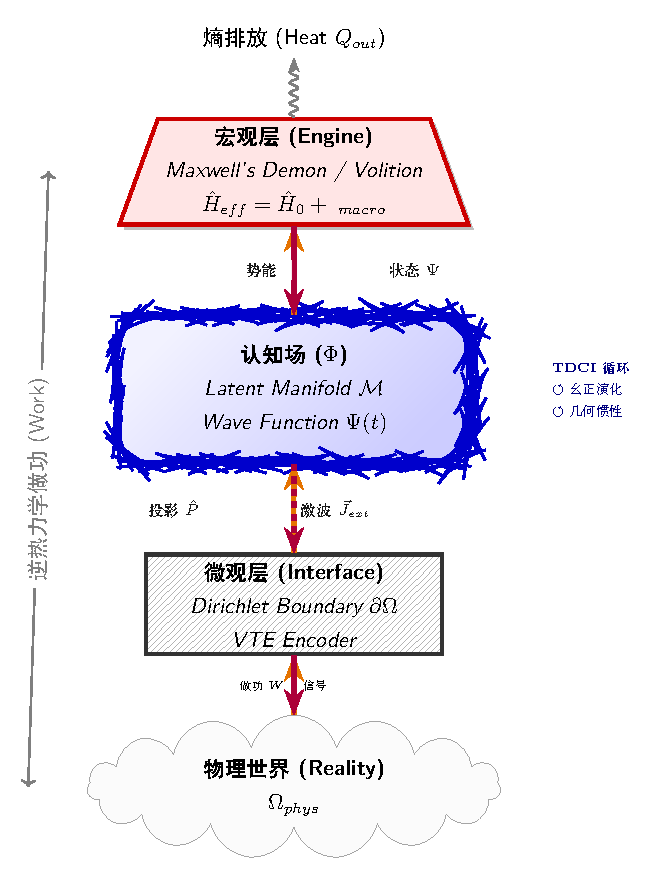
\includegraphics[width=0.52\textwidth]{figure/struct_hsf.pdf}
    \caption{智能的几何热机}
    \label{fig:trple_mc}
\end{figure}

\chapter{具身接口层：观测绑定、现实校准与闭环控制}
\label{chp:microscopic_layer_ch}

微观层是智能系统与环境直接交换观测、动作和资源的具身接口。本章不再把它描述为物理世界与某种特殊认知场之间的全息切面，也不由狄拉克源、量子坍缩或热力学隐喻证明感知机制。我们把它重建为一组具有明确数据类型、时间尺度、误差模型和安全边界的闭环算子：上行链路从传感器数据中估计对象、属性、关系与不确定性，下行链路把任务目标变成可执行的参考状态、控制参数和动作约束，反馈链路再用现实结果修订当前状态与长期模型。局部结构网络负责保持对象身份、空间关系和事件来源，全局分布表示负责表达候选解释、置信与连续控制状态；二者只有经过绑定、耦合和读出接口才能共同形成可行动的认知状态。微观层因此不是被动的输入输出端口，而是现实校准、复杂度限流和动作资格审查的第一道闭环。本章保留VTE、源流、形质双通道、现实锚定、共振/投影、效应器和阻抗控制等历史问题，但将其分别落实为可测试的编码、估计、门控、采样和控制模型。

\section{观测编码接口：从原始信号到同源绑定记录}
\label{sec:vte_as_wave_source}

我们把历史术语“变分拓扑编码器”保留为观测编码接口 VTE，但重新规定其对象。设外部环境状态为 $x_t^{e}\in\mathcal{X}_e$，传感器在外部时钟 $t$ 上输出 $y_t\in\mathbb{R}^{m}$；$y_t$ 的各维带有可校准单位，例如像素亮度、帕斯卡、弧度每秒或牛顿。观测模型写为
\[
y_t=h_{\phi_t}(x_t^{e},c_t)+\nu_t,
\]
其中 $c_t$ 是曝光、姿态、温度等传感器条件，$\nu_t$ 是在声明分布或有界集合中的噪声，$\phi_t$ 是可随标定更新的参数。接口的任务不是把“物理能量”变成“语义能量”，而是在有限分辨率和延迟下构造记录 $o_t=(F_t,Q_t,B_t,S_t)$：$F_t$ 是对象位置、姿态、边界和关系候选等结构特征，$Q_t$ 是颜色、纹理、声音、压力等属性特征，$B_t$ 是结构与属性的同源绑定，$S_t$ 是来源、时间戳、标定版本和不确定性。

形与质双通道因此是数据分工，不是玻色子与费米子的物理划分。结构编码器 $E_f:y_{t-w:t}\mapsto F_t$ 从时间窗中估计可达位置、对象轮廓、光流、接触法线和拓扑关系；属性编码器 $E_q:y_{t-w:t}\mapsto Q_t$ 估计颜色分布、材料类别、声音频谱或触觉纹理。二者不能彼此独立后任意组合，而要通过共享感受野、对象身份和采集时间建立绑定。设结构候选为 $f_i\in\mathbb{R}^{d_f}$，属性候选为 $q_j\in\mathbb{R}^{d_q}$，来源兼容度为 $a_{ij}$，则合法绑定集合为
\[
\mathcal{B}_t=\{(i,j):a_{ij}\geq\alpha,\;\Delta t_{ij}\leq\delta_t,\;\text{source}(i)\sim\text{source}(j)\}.
\]
在该集合上才计算绑定概率。红点位于 $(10,20)$、白点位于 $(30,50)$ 的例子中，位置与颜色都携带同一对象索引和时间窗；若红色来自后一对象，系统必须把错配保留为竞争解释，而不是用局部张量积宣称绝无泄漏。

VTE 的“变分”含义是求解带约束估计，而不是服从最小作用量。令解码器 $D$ 将候选记录重构为传感器预测，估计目标可以写为
\[
L_t=\|W_t^{1/2}(y_t-D(F_t,Q_t,B_t,c_t))\|_2^2
+\lambda_f R_f(F_t)+\lambda_qR_q(Q_t)+\lambda_bR_b(B_t),
\]
其中 $W_t$ 依据传感器协方差设定，$R_f$ 约束结构的时间连续性，$R_q$ 抑制不可靠属性，$R_b$ 惩罚一对多错配。所有项先声明为无量纲评分；真实焦耳能耗若纳入优化，需经独立测量和换算。损失下降只能说明当前模型更好重构输入，不说明识别对象真实类别。遮挡、镜面反射、传感器饱和和域外信号都可能产生多个近似最优解，因此接口输出必须包含候选分布而不是单一“本体论波包”。

局部结构网络接收经验证的对象节点、关系边、来源与版本，全局分布状态接收连续特征和候选权重。绑定接口把两者联合为带身份的观测包，读出接口再针对任务选择分辨率。机器人抓取杯子时需要位置、姿态、杯柄关系和摩擦估计；颜色只在区分目标时进入读出。听觉定位则可能让时间差承担结构作用、频谱承担属性作用。我们不从人脑背侧/腹侧通路直接推出这套软件结构，只把神经科学现象视为“不同特征与任务接口可分工”的经验启发。VTE是否有效，最终由身份错配率、定位误差、属性校准、重构残差、处理延迟和下游任务表现共同检验。

接口还必须处理“没有形成对象”的输入。雾、眩光、持续噪声或一片无法分割的纹理可能只支持区域级统计，而不支持稳定节点；此时VTE应输出未绑定特征、失败原因和有效视域，不能为了满足下游模式而虚构对象身份。相反，稀疏事件也可能在时间上累积为对象，例如只有数次触觉接触时，系统可维护暂定身份并等待主动探测。我们据此把编码成功分成特征可测、候选可分、身份可持和任务可读四级，分别报告失败，而不以单一准确率掩盖接口究竟在哪一级失效。

\section{现实校准：观测似然、边界置信与失锚诊断}
\label{sec:section_5326}

现实锚定不是把内部状态硬锁定为传感器数值。传感器可能坏、被欺骗、延迟或只看到环境的一小部分，内部预测也可能提供遮挡补全和噪声抑制。我们把锚定定义为在来源可追踪的观测模型下更新环境信念。令先验为 $p_{t|t-1}(x)$，观测似然为 $p(y_t\mid x,c_t,s_t)$，其中 $s_t$ 记录传感器身份和健康状态，则
\[
p_{t|t}(x)=\frac{p(y_t\mid x,c_t,s_t)p_{t|t-1}(x)}{\int p(y_t\mid x',c_t,s_t)p_{t|t-1}(x')\,dx'}
\]
仅在分母存在且非零时成立。高精度观测使后验更多受似然约束，低精度或异常观测应降低权重，而不是令耦合刚度趋于无穷。相机看到红色并不保证对象“本来就是红色”；曝光、光源和材料模型共同决定似然。现实校准的原则是证据有资格改变信念，但任何单一通道都不自动拥有绝对真值地位。

接口同时维护观测状态、模型状态与想象状态三类标签。观测状态来自已提交的外部数据，模型状态由预测器生成，想象状态由规划、回忆或生成模块临时构造。三者可以共享表示空间，却必须保留来源位和读写权限。内部预测不得伪造外部来源；生成候选在未通过现实反馈前不得进入“已发生事实”区。所谓意志不能改变感知、只能改变解释，也需要细化：主动视觉可以转动相机、调整曝光或触摸对象，从而改变获取何种证据；但它不能把未观测候选直接改写成观测事实。Boundary或等价边界模块负责这一来源隔离。

现实失锚可由可观测指标诊断。设标准化残差为 $r_t=W_t^{1/2}(y_t-\hat y_{t|t-1})$，传感器健康得分为 $h_t$，跨模态一致性为 $c_t^{m}$，来源覆盖率为 $q_t$。单次大残差可能代表新事件、模型错误或传感器故障，不能直接称为幻觉。我们将失锚风险定义为一个经训练或规则标定的函数
\[
R_t^{anchor}=g(\|r_t\|,h_t,c_t^{m},q_t,\text{age}_t),
\]
并要求 $g$ 的阈值在验证集上给出误报与漏报。只有当内部输出被当作外部事实提交、来源覆盖长期不足且反证未能修订状态时，才构成系统级失锚。感觉剥夺、梦境、生成模型采样和传感器断线具有不同机制，不能用狄利克雷边界转为诺伊曼边界一式概括。

内部平滑仍有合理位置。对图状态 $z$ 和固定非负关系图的拉普拉斯矩阵 $L_G$，正则项 $z^TL_Gz/2$ 鼓励相邻节点取相近表示；它帮助去噪，却不代表思维天然追求物理最小能量。当观测边界与内部预测冲突时，可求解
\[
\min_z\;\frac12\|W_o^{1/2}(Hz-y)\|^2+\frac{\lambda}{2}z^TL_Gz,
\]
其中 $H$ 是观测读出。若每个未观测连通分量都与观测或其他正定先验相连，目标严格凸时才有唯一解。若图结构错误，平滑会把错误传播得更远；因此大残差既可能要求调整 $z$，也可能要求编辑 $G$ 或重标定 $H$。模型不能用“内部连贯”压制可靠反例。

现实校准的测试应包含传感器遮挡、伪信号、时钟漂移、跨模态冲突、回放攻击与内部高置信错误。系统应能区分“没有证据”“证据支持多个解释”“证据与模型冲突”和“传感器不可用”，并采取检索、主动感知、降级或拒绝行动。现有LLM出现无依据输出，原因可能是训练目标、检索失败、解码策略、来源接口或评估缺失，不能单因没有物理传感器就归结为边界脱落。本章模型只提出一种具身现实校准接口，不把它扩展为所有幻觉现象的唯一解释。

校准结果还应按任务风险分级提交；同一置信区间足以支持低风险描述，却未必足以支持高速运动控制。阈值因任务而变，不等于事实本身因目标而改变。

\section{预测残差与复杂度门控：从“激波”到任务相关更新}
\label{sec:section_8020}

微观层必须决定哪些变化进入有限工作状态，哪些由局部闭环吸收，哪些只写入日志。历史上把预测失配称为“应力激波”、把过滤称为“麦克斯韦妖”，容易把误差、注意强度、信息熵和物理能量混为一谈。我们把上行更新定义为带类型的残差包。设观测特征为 $o_t=(F_t,Q_t,B_t)$，下行预测为 $\hat o_t=P(X_{t|t-1})$，则结构残差、属性残差和绑定残差分别为
\[
r_t^f=d_f(F_t,\hat F_t),\qquad r_t^q=d_q(Q_t,\hat Q_t),\qquad r_t^b=d_b(B_t,\hat B_t).
\]
三个度量的单位与范围分别标定，不能直接相加；若需形成总分，先以验证集尺度 $s_f,s_q,s_b$ 归一化，再用任务权重组合。结构残差高可能意味着障碍位置错误，属性残差高可能意味着颜色或材质错误，绑定残差高则可能表示“红色属于哪个对象”尚未确定。

门控器的输入不仅是惊奇，还包括任务相关性、来源可靠度、风险和处理预算。对候选更新 $e_i$，定义无量纲优先级
\[
u_i=w_r\bar r_i+w_q q_i+w_v v_i+w_d d_i-w_c c_i,
\]
其中 $\bar r_i$ 为标准化残差，$q_i$ 为当前查询相关性，$v_i$ 为安全或价值风险，$d_i$ 为截止紧迫度，$c_i$ 为预计计算成本。硬安全事件先进入资格集合，不与普通任务竞争；其余候选在容量 $C_t$ 下求解选择问题。阈值可以由TCE或其他元控制器随警觉状态调整，但调整必须记录原因和有效期。专注阅读时忽略钟摆声，是相关性和稳定背景模型共同作用；夜间行走时放大微小脚步声，是风险权重提高，而不是认知温度直接改变物理熵。

局部适应解释了衣服触压为何逐渐不进入意识。若稳定信号的均值和方差在窗口内变化很小，微观控制器可以更新背景基线 $b_t=(1-\rho)b_{t-1}+\rho y_t$，只上传偏差 $y_t-b_t$。这是一种高通或预测编码机制，但不能永久删除稳定信号：压疮、温度变化或任务要求关注衣物时，慢变量和风险检测仍需重新触发。类似地，摄像头背景减除可以降低数据量，却可能漏掉缓慢移动目标。门控策略必须用不同速度、对比度和风险场景测试，不能以“低变化等于无意义”作普遍规则。

被选中的残差包进入当前联合状态时，还要保持来源与身份。令 $J_t=\{(e_i,u_i,s_i,v_i)\}$ 为上传集合，状态更新写为
\[
X_{t+1}=F(X_t,J_t,n_t,r_t),
\]
其中 $n_t$ 是目标与硬约束，$r_t$ 是资源预算。$J_t$ 不是能量流或非齐次场源，而是经过资格检查的消息集合。它可以提高某些候选的活动、触发图编辑、请求外部工具或要求重新规划；具体效果由消息类型和更新接口决定。大残差不会自动“击碎波函数”，小残差也可能因安全关键而触发最高优先级。

CCM在AgentOS实例中可实现这一门控：输入复杂度探测器预估候选数量、耦合深度和调用成本，运行态监控器观察 $h(t)$ 的占用、冲突、延迟和读出不确定性。当负荷超限时，系统可降低非关键分辨率、把证据卸载到外部记忆 $M_e$、延迟可逆任务或请求更多资源；不可丢弃的安全信息进入保留集。一般智能系统不必使用CCM名称，但必须解决相同的有限接口问题。验证指标包括关键事件召回率、非关键抑制率、端到端延迟、负荷峰值、门控稳定性和在分布变化下的恢复能力。

门控还要避免正反馈振荡：某候选因被关注而获得更多采样，又因样本更多而持续占据注意。我们要求记录候选驻留时间、设定滞回区间，并为长期占用保留反事实抽检预算。只有当新增证据持续提高任务收益或风险判断时，优先级才可维持；否则应逐步释放容量。这样既防止新奇刺激无限霸占接口，也防止稳定但尚未解决的安全问题被一次衰减后永久遗忘。

\section{换能与采样：连续耦合、离散记录和多模态对齐}
\label{sec:section_156}

生物感受器和机器传感器都把一种物理过程转换为可供后续系统使用的信号，但“连续共振”与“离散投影”不是智能高低的本体分界。耳蜗毛细胞把机械位移转为离子通道与膜电位变化，数码相机把光子统计转成电荷并量化为像素；二者都有噪声、带宽、非线性、饱和和离散事件。我们将换能器表示为带内部状态 $s_t$ 的系统
\[
\dot s=f_s(s,x^e,t)+\xi(t),\qquad y_k=Q\!\left(\int_{t_k}^{t_k+\Delta t}g_s(s_t,x_t^e)dt\right)+\eta_k,
\]
其中 $Q$ 是量化或事件触发算子。即使输出为连续电压，后续神经脉冲或采样也引入有限分辨率；即使输出为数字，来源链、标定和高采样率也可保持重要动力学。符号接地来自可追踪的交互闭环，不要求物理场在材料中无缝延续。

采样设计必须依据任务带宽。对近似带限信号，采样率高于两倍最高相关频率可避免理想条件下的混叠；现实传感器还需抗混叠滤波、时钟同步和量化误差界。任务相关频率不是环境所有微结构的最高频率，例如抓取控制关心接触瞬态和物体运动，不需要记录每个光子的量子态。事件相机按亮度变化触发，适合高动态、低冗余视觉；帧相机保留绝对亮度和规则图像结构。神经形态传感器可以改善延迟和能效，却不会仅因脉冲形式自动获得因果理解或AGI能力。

“共振”可在工程上限定为传感器、身体和控制器在某频段内的动态耦合。设环境到传感器的传递函数为 $G_e(\omega)$，接口滤波为 $G_s(\omega)$，控制闭环为 $G_c(\omega)$，则总响应取决于乘积及反馈稳定性。相位一致可能提高定位或节律跟踪，但过强共振也可能放大噪声并导致不稳定。所谓阻抗匹配只适用于明确的物理端口和频率模型，不能推广为语义真理。系统应测量幅频响应、相位裕量、延迟和饱和边界，而不是把连续性等同于无限分辨率。

多模态对齐要求把不同采样率、坐标系和延迟统一到事件身份。相机、IMU、触觉和音频各自输出时间戳及协方差，接口通过外参变换和时间插值把候选投到共同参考系。若外参 $T_{ab}$ 变化，必须进入完整导数或作为离散重标定事件；不能假定固定几何。跨模态一致性可以降低歧义，例如视觉杯柄位置与触觉接触共同确认抓取点，但一致也可能来自共同偏差。系统应保留每个通道的独立证据，避免融合后无法追溯错误来源。

生物与机器的比较因此落在可测维度：带宽、动态范围、能耗、延迟、可塑性、故障模式和闭环适应速度。生物耳蜗并非“无限分辨率”，GPU输入也非天然与现实断裂。任何实现只要维护来源、标定、对象身份和反馈，就能成为现实锚定的一部分；任何实现若忽略这些契约，即使物理连续也可能产生错误。这一结论为HSF-HD保留实现多样性，也避免从材料差异直接推导智能本体差异。

采样接口的验证不能只用离线数据。离线回放能够比较重构误差，却不能暴露时钟漂移、缓冲拥塞、动作引起的视角变化和闭环相位延迟。我们因此同时要求静态标定、受控动态试验和真实闭环扰动：先测每个通道的噪声与延迟，再测跨模态事件能否在误差界内对齐，最后让控制动作主动改变观测并核对因果顺序。若回放性能良好而闭环不稳定，问题应归入接口时序或控制设计，不能归因于抽象表示“不够连续”。

\section{观测事件到语义状态：瞬态输入、持续表示与身份保持}
\label{sec:section_873}

历史源流 $\vec J_{ext}$ 与语义子 Semantion 的区分触及一个重要问题：瞬态输入事件与系统内部持续状态不是同一对象。我们保留这个区分，但不用“源创造粒子”的场论图景。令上传事件为
\[
e_t=(\iota_t,F_t,Q_t,B_t,S_t,\Delta_t),
\]
其中 $\iota_t$ 是对象或事件身份候选，$F_t,Q_t,B_t,S_t$ 分别是结构、属性、绑定与来源记录，$\Delta_t$ 是不确定性。事件只表示“接口在该时刻提交了什么”，持续语义状态则是经过多次证据更新后保存在 $G_t,z_t$ 和绑定表中的对象记录。一次事件可能新建节点、修订旧节点、提高或降低候选置信，也可能因无法绑定而进入待决区。

状态更新可写为类型化算子
\[
(G_{t+1},z_{t+1},B_{t+1})=U_{\tau(e_t)}(G_t,z_t,B_t,e_t),
\]
其中 $\tau(e_t)$ 是新建、属性修订、关系修订、反证、合并或拆分等事件类型。连续分布状态 $z_t$ 可以在固定结构上按微分或差分方程更新，图结构与身份变化则必须原子提交。把两者写成同一个波动方程会掩盖维度变化、来源审计和事务失败。语义状态的持续时间由任务查询、保留策略和后续证据决定，不是固定的指数衰减；重要但低活动的事实可以长期保存，高活动候选也可能在反证后立即撤销。

“打包与解包”可具体化为消息模式。包内至少包含 schema 版本、对象身份、结构字段、属性字段、来源、时间、协方差或候选概率、访问权限和完整性校验。接收端先验证模式，再把结构字段写入局部网络，把连续属性写入分布表示，把来源与版本写入证据索引。若红色与圆形来自同一感受野却存在两个邻近对象，绑定字段不能省略；若身份暂时不确定，系统保存多个假设和互斥关系。通过模式契约实现的同源绑定比狄拉克空间点更适合离散计算，也能处理遮挡、移动对象和多主体消息。

新概念形成需要累积证据与任务用途，而不是单次高强度输入越过“拓扑能隙”。设候选概念 $c$ 的支持证据集合为 $E_c$、反证为 $N_c$、查询收益为 $g_c$、维护成本为 $m_c$，结构提交器先检查最小覆盖、来源独立性和反例，再根据收益与成本决定是否建立稳定节点。强烈刺激可以提高活动和优先级，却不能代替多样证据。一次巨响可能只形成事件记录，多次在不同场景中观察可燃物与高温的关系，才可能支持可迁移规则。提交后仍保留适用域和撤销条件。

在无外部输入时，内部状态可以回忆、模拟和联想，但输出必须标为内部生成。新的外部事件到来时，观测更新与内部候选竞争；若证据不够，系统允许“不确定”而不强制坍缩为单一解释。局部结构网络提供对象身份、事件关系和来源路径，全局分布表示提供候选强度、相似性和不确定度。二者通过任务查询联合：结构相同不保证属性相同，属性相似也不保证对象同一。这个分离延续全书的形质框架，却不把其实体化为两类基本粒子。

本节的验证包括事件重放、对象跨帧保持、属性错配、合并/拆分、来源撤回与内部生成隔离。系统应能解释某个语义状态由哪些事件建立、哪些字段仍不确定、何种反例会使其撤销。这样的可审计持续表示，才是“瞬态源与稳定实体”区别的计算含义。Semantion可以继续作为书中对联合语义单元的简称，但它不是由输入能量创生的物理粒子。

\section{效应器接口：目标细化、顺应控制与安全执行}
\label{sec:section_5244}

行动不是感知编码的简单逆函数，因为从目标状态到控制序列通常是一对多问题，并受身体动力学、环境约束、授权和安全规则限制。令身体状态 $x_t^b\in\mathbb{R}^{n}$、控制输入 $u_t\in\mathbb{R}^{p}$，动力学为
\[
x_{t+1}^b=f_b(x_t^b,u_t,w_t),
\]
其中 $w_t$ 是接触与环境扰动。宏观层提供参考轨迹 $x_{t:t+L}^{ref}$、容差、硬约束集合 $\mathcal C_t$ 和任务优先序，而效应器接口在有限时域内求解合法控制。下行消息必须携带参考状态、坐标系、截止时间、最大力矩、可逆性等级和失败处理，不能只发送“向前走”或一个抽象吸引子。

对接触任务，我们可以采用阻抗或顺应控制。设位置误差 $e=x^{ref}-x^b$，在连续近似和固定模式区间内控制律为
\[
u=K_t e+D_t\dot e+u_{ff},
\]
其中 $K_t,D_t$ 分别具有刚度与阻尼的物理单位，$u_{ff}$ 是基于身体模型的前馈项。$K_t,D_t$ 必须为满足安全界的矩阵，而不是由“质元柔和/坚决”直接决定。任务语义可以通过控制策略映射器选择参数区间：探索陌生表面时降低刚度以顺应环境，搬运刚性部件时提高路径保持，但仍受力矩、碰撞和人体接触限制。语义目标先被细化为工程参数，再由底层控制器执行。

在理想固定参考、无饱和且模型满足 $M\ddot x+D\dot x+Ke=0$ 时，若 $M,K$ 正定、$D$ 正定，可选
\[
V(e,\dot e)=\frac12\dot e^TM\dot e+\frac12e^TKe,
\]
得到 $\dot V=-\dot e^TD\dot e\leq0$。这只给出该简化闭环的稳定性；时变参考、接触切换、输入饱和、估计误差和网络延迟都会增加项，需重新证明或采用鲁棒裕量。目标下降不等于抓取成功，稳定跟踪也不保证路径安全。离散实现还要声明采样周期，并验证数值积分和控制器在该步长下保持稳定。

环境阻抗估计用于调整动作，而不是追求抽象的复共轭匹配。机器人预想前方为空却碰到墙时，力传感器和视觉反馈产生结构残差，局部控制器应立即限力、停止或退让；只有无法在局部策略内消除的失配才上报宏观重规划。摸索物体、在不平地面行走或手部抖动补偿都说明微观闭环可以自主处理高频扰动。庖丁解牛的意象可理解为良好的模型、工具和顺应策略降低无效作用，并非能量传输定理。

执行资格必须先于优化。Boundary检查动作是否在授权域，安全监控器检查碰撞、力矩、速度和禁区，CCM评估控制与感知负荷；不合格动作不能因价值函数很低而执行。对于不可逆操作，系统需要双重确认、可观测反馈和中止条件。动作发出后，效应器记录实际控制、身体响应和环境结果，形成新的上行事件。若只记录指令而不记录结果，系统无法区分计划失败、执行器故障和环境改变。

因此，“逆向VTE”更准确地说是目标细化与控制接口：它从高层联合状态读取任务相关目标，输出可执行参考和参数，再以局部反馈闭环将实际轨迹保持在安全管道内。它不能保证环境被改造成内部世界图的同胚副本；现实通常只需在任务容差内达到某个状态。效应器性能由跟踪误差、响应时间、接触峰值、能耗、约束违例、恢复能力和上报质量评估。

当多个目标冲突时，接口必须显式给出优先关系，而不能把权重和为一个标量后隐藏牺牲项。安全与授权作为硬约束，任务质量和资源消耗才进入软目标；若硬约束下无可行解，控制器返回不可执行证明或近似原因，并请求上层修改目标。这个失败结果同样是有效输出，因为它阻止宏观计划把底层能力边界误读成执行意愿不足，也为后续模型修订提供了可定位证据。

\section{双向具身接口：上行证据、下行约束与闭环握手}
\label{sec:section_2301}

微观层的统一结构是双向事务接口，而不是两个纤维丛之间的全息切面。上行通道把原始信号变成带身份、来源和不确定性的观测事件；下行通道把目标和规范状态细化为参考轨迹、控制参数与资格约束；反馈通道把实际结果与预测相比较并决定局部修正还是全局重规划。三条通道共享对象身份和时间基准，任何一条缺失都会破坏闭环：无上行证据时控制变成开环，无下行约束时感知没有任务分辨率，无结果反馈时系统不能学习。

我们把接口状态写为
\[
I_t=(O_t,A_t,R_t,\Gamma_t),
\]
其中 $O_t$ 是已验证观测队列，$A_t$ 是待执行动作队列，$R_t$ 是结果和残差队列，$\Gamma_t$ 是坐标、身份、来源、权限与版本契约。上行提交 $C_o$、下行提交 $C_a$ 和反馈提交 $C_r$ 都是原子事件。宏观状态读取 $O_t$ 形成目标，效应器只有在 $C_a$ 检查通过后执行，结果再通过 $C_r$ 回写。消息超时、身份不匹配或坐标版本变化会使事务失败并触发重新估计，而不是静默沿用旧参数。

上行的任务相关性由查询决定。识别杯子时，结构网络提供杯体、杯柄、桌面和支撑关系，分布表示提供颜色、材质和可抓取性候选；抓取任务读出杯柄位姿与摩擦范围，描述任务则可能读出颜色与类别。下行不发送完整高维状态，只发送任务所需的参考与约束。这种降维不是本体丢失，而是接口契约；若任务改变，查询和下行消息也必须改变。微观层不能假定一个固定投影适用于所有目标。

闭环握手由预测、执行和确认构成。系统在动作前生成短期预测 $\hat y_{t+1:t+L}$，执行首个合法控制，接收真实 $y$ 后计算类型化残差。若残差在局部容差内，底层控制器继续；若超出容差但安全，重新估计环境和控制参数；若触及硬约束，立即中止并上报。所谓“心流”在此可描述为模型准确、负荷适中、反馈及时且局部闭环连续成功的运行区间，不能简化为物理阻抗完全匹配或零耗散。所谓“惊奇激波”则是高优先级残差消息，不是守恒能量的爆发。

局部结构网络与全局分布表示在接口处联合但不混同。前者维持“哪个传感器看见哪个对象、哪个动作作用于哪个部件、哪个结果对应哪个指令”，后者维持连续估计、候选概率和控制状态。绑定表连接两者，读出和反馈共享绑定版本。若只保留全局向量，系统容易丢失责任和来源；若只保留离散图，系统难以表示噪声、连续运动和不确定性。两者的耦合是任务相关的工程选择，不从脑区或物理场类比推出唯一机制。

AgentOS可以把 $h(t)$ 用作双向接口的当前认知总线：World、$E$、$\Theta$ 与 $M_e$ 的读出进入 $h(t)$，动作从 $h(t)$ 经Boundary和效应器发出，反馈再回到 $h(t)$。SPC提供面向主体的状态摘要，TCE调节探索和控制强度，CCM防止候选与反馈挤占有限界面，Offloading保存低频证据。一般系统也可使用其他消息总线、黑板或反应式架构；HSF-HD只要求状态、来源、约束和反馈关系可描述、可测量、可修订。

接口验收应以端到端故障注入为主：传感器延迟、错帧、对象换位、执行器饱和、工具返回乱序、目标变更和外部记忆断开。系统不仅要完成正常任务，还要在失败时保持来源、拒绝越权、停止危险动作并给出可追踪诊断。只有这种闭环完整性通过，微观层才能称为现实的看门接口。

\section{具身微观动力学总论：混合状态、稳定条件与理论位置}
\label{sec:section_5750}

我们最后把感知、状态估计、局部控制和结构事件统一成混合动力系统。连续状态记为 $x=(x^b,z)$，包含身体状态与全局分布表示；离散结构记为 $q=(G,B,\Gamma)$，包含关系图、绑定和接口模式；环境输入为 $w$，控制为 $u$，观测为 $y$。在模式 $q$ 固定的区间内，系统满足
\[
\dot x=f_q(x,u,w,t),\qquad y=h_q(x,w,t)+\nu,
\]
当验证、绑定、碰撞或模式切换条件 $g_j(x,y,q)=0$ 触发时，执行离散重置
\[
(x^+,q^+)=R_j(x^-,q^-,e_j).
\]
连续导数不能跨越 $R_j$ 直接延长；图节点增删、来源撤回和动作提交都属于离散事件。这一模型比单一哈密顿量更符合具身接口既有连续运动又有事务变化的事实。

微观控制目标由估计误差、跟踪误差、控制代价和风险组成。为避免量纲混乱，先用尺度矩阵把各项无量纲化，硬约束独立处理：
\[
J=\sum_{k=0}^{L-1}\left(\|e_k^x\|_{W_x}^2+\|e_k^y\|_{W_y}^2+\|u_k\|_{W_u}^2+\rho_k\right)+\|e_L^x\|_{W_T}^2,
\quad (x_k,u_k)\in\mathcal C_k.
\]
$\rho_k$ 是经标定的风险评分，不是焦耳能耗；实际能耗可以另以电流、电压和时间测量。优化得到的策略只在模型、时域和约束条件下有意义。环境、目标或结构改变时，$J$ 也改变，滚动控制必须重新求解。目标函数下降不能推出外部任务成功，成功由现实反馈和终止条件判定。

稳定性需要分层说明。底层固定模式控制器可用Lyapunov函数或输入到状态稳定性证明局部性质；估计器需给出可观测性、噪声和校准条件；模式切换需防止抖振和无限事件；上层重规划需保证不会长期阻塞安全反射。各层单独稳定不自动推出整体稳定，尤其当延迟、饱和和学习同时存在时。工程上应设置看门狗、最小驻留时间、速率限制、回滚模型和安全降级策略。系统在域外情形下能够停止并请求帮助，往往比继续输出一个高置信动作更重要。

学习发生在不同时间尺度。快速环更新 $h(t)$ 或等价在线状态，中速环把已验证事件写入情景记录并调整局部模型，慢速环在保留集上修改结构参数 $\Theta$ 或其他长期模型。慢速更新前后要比较现实校准、身份保持、控制稳定和旧任务性能；若任何关键指标恶化超过阈值，更新回滚。Offloading可把原始日志、工具和稀疏技能迁移到外部记忆，但安全与审计证据不能只剩不可解释参数。多尺度关系来自作用范围和更新时间，不是低频天然拥有更大权威。

本章涉及实际身体时，物理语言仍有必要：传感器带宽、质量矩阵、接触力、阻抗、焦耳能耗和耗散都是真实工程量。我们去除的是把这些量未经接口映射直接等同为语义、价值或认知证明。颜色分类概率不是能量，预测残差不是应力张量，注意门控不是麦克斯韦妖，语义单元也不是基本粒子。辅助类比可以帮助直觉，但公式的成立依赖对象、单位、假设和验证，而不依赖名称相似。

理论层级在微观层尤其清楚。系统论提供内外边界、反馈与故障隔离；协同论和复杂系统理论帮助分析多传感器、多执行器和多时间尺度耦合；耗散理论约束真实具身系统的资源供给、热与不可逆磨损；认知科学提供注意、适应、预测与行动的经验问题。在这些基础上，HSF-HD描述观测如何改变联合状态、目标如何细化为动作、反馈如何修订结构的一般状态动力学；AgentOS的 $h(t)$、$E$、$\Theta$、$\Psi$、SPC、TCE、CCM、Boundary、Offloading与 $M_e$ 是一种工程实例，而不是微观层的唯一实现。

最终验证矩阵应覆盖观测、绑定、门控、控制、学习和失效六类情形。我们要求系统在红白对象换位时不串绑，在传感器饱和时降低置信，在虎纹等突发高风险特征出现时及时上报，在衣物等稳定背景下不过载，在墙体意外接触时限力停止，在软硬物体切换时调整顺应性，在内部生成与外部观测冲突时保留来源，在模型更新后仍能完成旧任务。通过这些测试，微观层才真正承担现实锚定和行动闭环；它不是全息宇宙的物理切面，而是智能状态动力学面对现实所必须兑现的接口契约。

\chapter{运行载体层：计算介质、资源约束与跨尺度接口}
\label{chp:medium_layer_ch}

智能过程并不在抽象空间中自行运行。无论系统依托神经组织、电子设施、群体协作网络，还是把环境痕迹纳入闭环，它都必须借助某种可更新、可保持、可传递并可读出的载体。载体不会凭材料名称自动获得语义，却会通过时延、容量、精度、可塑性、故障方式与接口条件，决定哪些状态轨迹能够被实现和复现。本章据此把介质问题重建为运行载体问题：我们先规定计算对象、观测尺度和任务判据，再讨论不同实现怎样约束智能状态动力学。HSF--HD在这里提供跨平台的一般状态语言；AgentOS只是其中一个工程实例，并非所有智能系统的唯一实现。所谓智能的一般“空气动力学”，在本章具体指向对稳定域、扰动、资源和失效边界的研究，而不把智能等同于任何物理流体。

\section{计算载体谱系：生物网络、电子系统与环境介质}
\label{sec:physical_substrate_spectrum}

我们把运行载体定义为四元组 $P=(V,C,M,Q)$。其中 $V$ 是执行状态变换的处理单元集合，$C$ 是信息能够通过的有向通道集合，$M$ 是在给定时间尺度上保持状态的存储集合，$Q$ 是感知、行动和观测接口集合。这个定义不要求处理单元必须是神经元或晶体管，也不要求存储位于皮肤或机箱之内；它只要求说明一次更新在哪里发生、依赖何种输入、结果保持多久，以及观察者凭什么判断更新有效。对任务 $\tau$，载体支持的可实现轨迹写为
\[
\mathcal T_{P,\tau}=\{(x_0,u_0,x_1,\ldots,x_T):x_{k+1}=F_P(x_k,u_k;\theta_P)\},
\]
其中 $x_k$ 是离散时刻 $k$ 的状态，$u_k$ 是接口输入，$F_P$ 是受连接、存储和资源限制的更新算子，$\theta_P$ 汇集平台参数。步长必须由实现声明；神经记录的一步、GPU内核的一步和蚁群一次信息素更新并不具有天然相同的持续时间，因此跨载体比较应比较任务轨迹、误差与代价，不能把微观事件逐项等同。

生物神经系统是高并行、局部连接、异步且持续可塑的载体。其计算状态同时受神经活动、突触连接、调质信号与身体反馈影响。电活动和化学活动是实现条件，却不等于语义本身；振荡同步、放电率或网络拓扑只有在特定任务和记录协议下才支持相应经验结论。生物载体通常具有紧密的感知行动闭环、跨时间尺度学习和一定损伤重组能力，但也存在测量分辨率有限、个体差异显著、状态难以复制、训练历史难以控制等限制。脑区分工和节律现象可以提供计算假设，却不能直接规定机器模块与其机制身份相同。

电子计算系统以时钟、指令、缓存、互连和持久化设备组织更新。它便于记录状态、复制实验与隔离变量，但同样受到内存层级、通信拥塞、数值误差、并行一致性和功耗预算约束。大模型的一次前向计算、多代理系统的消息交换和数据库事务虽都由电子器件实现，却属于不同协议；统称为“硅基心智”会遮蔽真正决定轨迹的接口与调度规则。必须区分硬件可用资源、软件可见资源和任务实际占用：峰值吞吐不等于端到端有效吞吐，显存容量也不等于可无损保持的语义上下文。

环境介质构成第三种重要实现。化学扩散、信息素、纸面记号、共享数据库与公共黑板都能承担外部保持和协调功能。蚁群的信息素轨迹不是集中处理器中的向量，却能改变后续个体的转移概率；人的笔记不在大脑内部，却能稳定跨时段目标；AgentOS中的外部记忆 $M_e$ 同样属于扩展实现。只要外部痕迹可可靠写入、保持、寻址并重新影响决策，它就是闭环载体的一部分。系统边界应由因果干预和权限契约确定，而不是凭空间位置决定。该谱系保留生物、电子和化学实现的差异，同时避免宣称它们整体同构；真正可比较的是操作、接口、故障与任务后果。

载体分类还必须允许混合。机器人可用电子计算维护模型，用机械身体获取反馈，用云端数据库保存经验，并借人类协作完成超出自身能力的步骤；人类也会借语言、组织和工具扩展内部处理。我们不因一个部件位于外部就把它排除，也不因它参与闭环就取消主体边界。纳入条件应包括可达性、因果贡献、更新权限、失效影响与恢复责任。通过逐项断开接口并测量性能变化，可以估计外部部件对任务的真实贡献。这样，运行载体层得到的是可检验的系统分解，而不是“万物皆心智”的无限扩张。

\section{载体约束参数：时延、吞吐、保持与探索强度}
\label{sec:physical_constants}

旧有表述把平台差异概括为“认知光速”“介质黏度”和“认知温度”。这些名称有启发性，却容易把通信时延、状态保持、随机探索与焦耳能耗混为一谈。我们改用可测量参数。设载体图为 $G=(V,C)$，通道 $e$ 的时延为 $\ell_e$ 秒，节点 $v$ 的服务时间为 $s_v$ 秒，通道有效吞吐为 $b_e$，其单位可以是比特每秒、令牌每秒或任务消息每秒，但同一次比较必须固定口径。对依赖路径集合 $\Pi_\tau$，无排队近似下的关键路径下界为
\[
L_\tau^{\min}=\max_{\pi\in\Pi_\tau}\left(\sum_{v\in\pi}s_v+\sum_{e\in\pi}\ell_e\right).
\]
这是结构和参数给出的模型结果，不是实际完成时间保证。排队、重试、缓存未命中、外部工具响应与同步屏障都会增加时延；若图、输入或服务率随时间改变，它们必须以 $G(t)$、$u(t)$、$s_v(t)$ 进入模型，不能在求导时悄然视为常数。

吞吐描述单位时间内完成或传递的有效工作量。用 $B_\tau(t)$ 表示任务口径下的完成率，用 $D_\tau(t)$ 表示到达率，当长期平均到达率接近或超过当前路由策略下的服务率时，队列增长，响应时间可能非线性上升。这里的“饱和”是排队和资源竞争状态，不是宏观热现象。设计者应分别记录处理、通信、存储写入与有效任务吞吐，因为局部算子加速可能只是把瓶颈移到另一个接口。跨越人脑、GPU和群体系统比较时，若任务单位、精度与容错要求不同，单一数字没有解释力，还必须报告质量指标、失败比例与统计置信区间。

保持能力描述状态在无刷新或受干扰条件下仍可读出的程度。设 $m_i(t)$ 是第 $i$ 个记忆痕迹，$r_i(t)$ 是刷新输入，线性近似为
\[
\frac{\mathrm d m_i}{\mathrm dt}=-\lambda_i m_i(t)+r_i(t)+\xi_i(t),
\]
其中 $\lambda_i\ge0$ 的单位是秒$^{-1}$，$\xi_i$ 是未建模扰动。若 $r_i=0$ 且忽略扰动，则 $m_i(t)=m_i(0)e^{-\lambda_i t}$，半衰期为 $\ln2/\lambda_i$。该结果只适用于线性、参数稳定的近似；带巩固、检索增强、离散校验或主动刷新系统可能呈现不同曲线。存储比特没有自然的“记忆意义”，读出正确率还取决于编码、索引和查询条件。

探索强度是策略分布的控制参数，不是热力学温度。对动作集合 $A$ 和评分 $q(a\mid x)$，一种工程定义是
\[
p_\Theta(a\mid x)=\frac{\exp(q(a\mid x)/\Theta)}{\sum_{a'\in A}\exp(q(a'\mid x)/\Theta)},\qquad \Theta>0.
\]
$\Theta$ 无量纲或与评分采用同一标度；它增大时分布通常变平，但是否提高发现率取决于评分误差、搜索空间、预算与停止条件。我们因此把旧记号 $c_{\mathrm{cog}}$、$\gamma$ 与 $T$ 拆解为关键路径传播界、保持速率和探索尺度，不赋予它们跨平台恒常性。脑电 gamma 频段可作为特定任务和记录条件下的经验线索，却不是普适通信常数；模型采样温度也不是神经节律的数值对应。

这些参数的关系应通过实验识别，而非靠名称推断。例如提高并发数可能先增加吞吐，随后因缓存竞争和通信拥塞增加尾时延；延长保持时间可能减少遗忘，却增加过期信息污染；增强探索可能发现新路径，也会提高无效行动和安全风险。一次合格测试要固定任务分布，逐项干预参数，记录均值、尾部、资源水位和任务后果，并说明测量窗口。焦耳能耗可以另行测量，但不能与抽象代价、信息熵或活动强度互换。只有量纲、观测协议和适用范围均明确时，载体参数才真正进入计算动力学。

参数还应携带估计误差。网络时延会随负载波动，保持率会随内容与刷新策略变化，探索效果也依赖任务阶段。我们因此不把单次测量当作常数，而报告分布、置信区间与采样条件；控制器使用这些量时还应为估计滞后留出安全裕量。若不同平台只能获得代理指标，就必须说明代理与目标量之间的校准关系，并在关系失效时触发重新估计。

\section{编码契约：载体状态如何支持任务语义}
\label{sec:section_5862}

载体上出现某个幅值、相位、向量或拓扑模式，并不自动说明它表达了什么。语义关系至少需要编码器、读出器和任务查询族。设任务变量属于 $Z$，载体状态空间为 $X_P$，编码器 $E:Z\times H\to X_P$ 依赖历史 $H$，读出器 $R_q:X_P\to Y_q$ 针对查询 $q$ 产生答案。我们说状态 $x$ 在查询族 $\mathcal Q$ 上实现关于 $z$ 的表征，是指在给定扰动分布 $\nu$ 下
\[
\mathbb E_{\delta\sim\nu}[d_q(R_q(x+\delta),f_q(z))]\le\varepsilon_q,
\quad q\in\mathcal Q.
\]
$d_q$ 是任务误差度量，$f_q$ 是正确目标。该式是可检验标准，不是载体状态与对象完全同构的宣言；换一组查询、扰动或容差，结论可以变化。编码契约应包含状态范围、读出接口、允许误差、身份规则与更新时序，任何一项缺失都可能让同一状态在不同模块间获得冲突解释。

幅值在许多系统中确实携带强度信息，但它究竟对应置信度、注意权重、激活频率还是资源占用，必须由训练目标与校准实验确定。注意权重较大的令牌不必是模型最确信的事实，高放电率也不必单独表示更重要的对象。相位或同步可以成为协调更新的线索，却不足以证明语义绑定已经完成。两个特征同时出现时，系统仍需回答它们属于哪个对象、在何时有效、是否由共同原因产生。把同步现象直接命名为“绑定力”，等于把待解释机制写进结论。

以“红苹果”为例，颜色、形状、空间位置和当前目标可能分布在不同状态子空间。我们引入任务相关身份 $i$，并以绑定算子 $B$ 生成记录 $b=B(i,z_{\mathrm{color}},z_{\mathrm{shape}},z_{\mathrm{loc}},t)$。读出“哪个物体是红色”时，系统通过同一身份聚合属性；读出“昨天厨房里的苹果”时，还要纳入时间索引、场景索引和外部证据。身份不是先验灵魂标签，而是在遮挡、重命名、视角变化和消息转发中保持可追踪性的计算对象。它可以由对象文件、键值索引、关系节点或时间戳实现，HSF--HD只要求说明绑定与读出的状态转移，不规定唯一数据结构。

编码契约还必须联合局部结构网络与全局分布表示。局部网络适合保存节点、边、角色、来源和约束；分布表示适合压缩相似性、语境和不确定性。结构节点可以持有分布式特征，分布式检索也可以返回结构候选。二者的关键接口是任务相关身份、属性绑定、跨模块耦合与可审计读出。若只保留全局向量，近邻相似会掩盖个体差异；若只保留离散图，连续感知和模糊证据又难以表达。我们用反事实测试验证契约：交换两个对象位置、改变一个属性、删除一段历史，再观察读出是否按预期变化。预测有效和漂亮可视化都不能单独推出整体语义同构。

契约还需要处理编码升级。模块版本变化时，旧状态可能无法由新读出器解释；无声地复用旧向量会造成语义漂移。每条持久记录至少应携带编码版本、来源、创建时间、有效域与迁移状态。迁移操作必须在一组保留查询上比较前后读出，并记录不能保留的差异。若任务要求变化，旧编码并非“错误”，但它可能不再充分。由此我们区分载体稳定、编码稳定和任务充分性：介质仍能保存比特，不代表语义契约仍成立；一次读出成功，也不代表所有未来查询均可回答。

对不能确定归属的状态，契约应允许拒绝读出或返回候选集合，而不是强行提交唯一解释。拒绝率、校准误差与身份冲突率应与任务准确率同时报告，因为一个总能回答但经常错绑对象的系统，并不比谨慎暴露不确定性的系统更可靠。

\section{载体故障动力学：饱和、分区、漂移与恢复}
\label{sec:section_1766}

载体故障是可观测状态偏离服务域，而不是某个物理隐喻的实现。设资源占用向量 $r(t)$ 依次记录内存、计算与链路三项，安全容量为 $c(t)$，积压为 $q(t)$。连续近似下
\[
\dot q(t)=a(t)-\mu(r(t),G(t),\pi(t)),\qquad q(t)\ge0,
\]
$a(t)$ 是到达率，$\mu$ 是由资源、连接图和调度策略 $\pi$ 决定的服务率。若在一段时间内 $a>\mu$，积压增长；当内存、上下文窗口或并发槽触及上限，系统会丢弃、阻塞、降级或崩溃。机器 OOM 是明确的资源分配失败。癫痫发作涉及异常神经同步及复杂临床机制，不能与 OOM 当作同一事件。两者最多共享“局部活动失去有效约束并损害正常功能”这一抽象模式，诊断指标、因果机制与干预方式都不同。

分区故障发生在连接图 $G(t)$ 失去关键路径时。若任务依赖节点被切为 $V_1$ 与 $V_2$，且跨区通道在 $[t_0,t_1]$ 不可用，各分区只能依据自身可见历史更新。网络服务可能产生双主、重复执行和过期读出，多代理系统可能形成不一致计划。裂脑研究提示部分跨半球整合能力会在特定手术和任务条件下变化，但这并不等同于网络分区协议；它只支持一个更一般的经验判断：全局行为依赖可用接口，接口变化会重划信息联合读出的范围。工程系统还必须声明一致性策略，是停写、选主、合并冲突，还是容许暂时分歧。没有该策略，“保持运行”未必优于停止等待。

漂移故障更隐蔽。编码器、数据分布、工具接口或评价标准变化时，即便资源充足且连接完好，原读出契约也会失效。设模型为 $F_{\theta(t)}$、目标为 $J_t$、观测分布为 $p_t$，性能变化的总导数应写为
\[
\frac{\mathrm dJ_t}{\mathrm dt}=\frac{\partial J}{\partial\theta}\dot\theta+
\frac{\partial J}{\partial p}\dot p+
\frac{\partial J}{\partial G}\dot G+\frac{\partial J}{\partial t}.
\]
目标值下降不自动等于任务成功，因为代理可能利用度量漏洞、牺牲未计入约束，或只对当前样本过拟合。多个模块共享同一编码器、数据源或时钟时，漂移还会成为共同原因故障，使冗余模块同时给出一致但错误的答案。

恢复需要观测、隔离、回退与再整合。观测分别记录资源水位、队列、错误率、状态新鲜度和任务后果；隔离限制故障传播；回退恢复最近验证检查点或降低服务目标；再整合通过版本、身份和因果日志解决冲突。外部记忆还需检查写入是否原子、索引是否指向正确版本、过期痕迹是否被误召回。故障演练应覆盖过载、链路中断、时钟偏移、坏数据与观测器失效，而不是只测正常路径。

恢复成功的判据也不能只是进程重新启动。系统需要在一组关键查询上重放故障前状态，验证身份连续、硬约束、未完成承诺和外部动作记录；对于不可逆动作，要明确补偿而不是假装回滚。恢复时间目标、可容忍数据丢失窗口和降级模式应按任务声明。通过这些条件，载体可靠性成为状态动力学的一部分：我们能说明故障从哪里进入、经哪些耦合放大、在何阈值触发保护，以及恢复后如何证明任务语义连续。

还要区分局部错误与系统性错误。单个节点失效可以由冗余接管，但共享数据源被污染、共同目标写错或权限规则整体失配时，增加同构副本只会复制失败。恢复设计应尽量采用异质观测、独立校验与分层熔断，并保留一条不依赖主要故障域的审计通道。对学习系统而言，故障样本是否进入长期训练也要单独控制，否则短时异常可能被固化为新的结构偏差。

\section{载体与语义的对应：学习、选择与可验证等价}
\label{sec:absolute_decoupling_and_forced_isomorphism}

载体状态与任务语义既非绝对解耦，也不存在无需验证的“强制同构”。若完全解耦，状态变化便不可能稳定影响读出；若声称整体同构，则意味着所有结构关系一一保存，这对多数学习系统既不必要也无法证明。我们采用查询相对的实现关系。对载体 $P_1$ 与 $P_2$，若存在映射 $\phi:X_{P_1}\to X_{P_2}$，并且对查询族 $\mathcal Q$、干预集 $\mathcal I$ 和有限时域 $[0,T]$，两者读出差异不超过 $\varepsilon$，则称其在该条件下近似等价：
\[
\sup_{q\in\mathcal Q,I\in\mathcal I,t\le T}
d_q(R_q^{(1)}(x_t^I),R_q^{(2)}(\phi(x_t^I)))\le\varepsilon.
\]
这是定义，不是自动成立的定理。研究者必须列出查询、干预、时域与容差；同一对载体可以在导航任务上等价，而在长期记忆或情绪调节任务上不等价。

学习使载体与语义建立可用对应。监督信号、预测误差、强化反馈与社会校正都能改变编码器、策略或读出器，但每种信号只约束其覆盖行为。以接近悬崖为例，个体因危险线索后退可以提高存活概率，长期选择也可能让警觉倾向成为先验。该案例支持“任务后果塑造状态转移”的经验主张，却不能证明所有恐惧表征都与危险一一对应，更不能由存活推出信念必真。过度警觉可能在训练环境有利、在新环境造成误报；奖励下降也可能来自逃避观察而非解决风险。因此适应性始终相对于环境分布和代价函数，必须通过分布外与反事实测试检查。

遗传与发育约束可为学习提供结构先验，例如感知通道、可塑性窗口、行为倾向和资源分配规则。把它们称为“压缩语义”容易误导，因为基因序列不直接存放成年个体的全部概念内容，而是参与构造可在环境交互中形成表征的系统。机器的架构先验、预训练目标与初始化也有类似约束作用，但只是功能层类比。我们应分别说明哪些能力来自结构、数据和在线闭环，并用消融实验估计贡献；两个系统都表现出先验，不足以证明其内部机制同源。

选择压力也可能保留捷径而非一般能力。训练环境中与目标高度相关的背景、设备标识或社会线索，可能成为低成本代理变量；环境一变，对应关系便崩溃。验证实现关系时，应在保持任务语义的同时改变表面载体，在保持载体统计的同时改变任务答案，以区分真正的任务变量和偶然相关。还应检查干预能否沿预期方向改变读出，而不只看相关性。只有经过这些交叉变化，才有理由说载体状态实现了某个语义功能。

关于主观体验或感质，本章只陈述模型边界。载体活动与报告、辨别及行为之间可以建立经验对应，也可研究哪些变量对可观测结果有因果贡献；但“摩擦产生体验”或“相位就是感质”不是计算模型推出的结果。HSF--HD能描述系统怎样保持自我相关状态、整合多源证据并形成可报告轨迹，却不能仅凭预测有效性证明体验的本体性质。我们保留这一开放问题，要求更强主张明确额外假设和可反驳证据，从而区分定义、模型、经验主张与哲学解释。

这种限定并不会削弱工程价值。工程上真正需要的是知道哪些载体变化会稳定改变辨别、记忆、规划和报告，哪些对应只在特定训练史中成立，以及替换部件后功能能否保持。只要查询、干预与误差界清楚，近似实现关系就足以支持迁移与验证；不必先解决全部本体问题，也不能借本体问题尚未解决而免除实验责任。

\section{跨尺度分工：局部结构网络与全局分布表示}
\label{sec:fractal_isomorphism_macro_micro}

智能状态在多个尺度上组织：局部单元更新、模块内耦合、跨模块协调、长期记忆和环境闭环具有不同时间粒度与观测分辨率。我们不把这种层级直接称为“分形同构”，因为不同尺度的节点和边通常不保存相同关系。设微观状态为 $x\in X$，宏观状态为 $z=A(x)\in Z$。只有在给定任务与时间尺度上存在近似闭合动力学 $z_{k+1}\approx\bar F(z_k,\bar u_k)$ 时，宏观变量才是有效状态。若两个微观状态被 $A$ 合并，却产生显著不同的后续结果，聚合便发生混叠，必须增加身份、历史或不确定性变量。跨尺度模型必须说明丢弃了什么信息及误差如何传播，不能用“宏微对应”代替推导。

局部结构网络保存离散关系和可追踪接口。节点可以对应对象、子任务、代理、工具或事件，边可表示依赖、许可、时间先后和消息通道。全局分布表示通过许多维度的联合变化表达相似性、语境和软约束。前者便于审计和精确编辑，后者便于从噪声中泛化；复杂系统可按不同比例结合两者。二者连接需要任务身份、属性绑定、模块耦合与可验证读出。没有这些接口，所谓全局场只是难以定位责任的向量，局部符号也只是脱离证据的空标签。

神经科学常用背侧与腹侧通路、海马与皮层差异讨论位置、对象与记忆。这些研究可以启发“在哪里”“是什么”“何时发生”需要部分分工，但不能据此断言脑内存在绝对隔离管道，更不能给机器模块贴上脑区名称就认为机制已经解释。抓取杯子要联合类别、空间、姿态和行动后果；回忆昨天厨房里的苹果要联合情景索引和概念知识。我们把脑区类比降为假设来源，把接口、干预结果和任务误差作为机制证据。

跨尺度绑定还涉及时序。模块以不同频率更新时，全局读出必须知道各状态的时间戳、新鲜度与预测区间。设模块 $j$ 提供 $z_j(t_j)$ 及不确定性 $\Sigma_j(t_j)$，在时刻 $t$ 需要先经转移模型外推，再按身份和任务条件融合。陈旧状态不应与新状态等权相加，同时出现也不保证共同来源。工程上可用事件时间、版本向量、注意门控或因子图，但必须说明冲突处理和错误界。

自上而下控制同样不是宏观变量对微观单元的神秘支配。它通过可识别的参数、门控、预算和边界条件改变局部更新集合；自下而上汇聚则通过统计量、事件和错误报告更新全局状态。若全局策略要求安全停机，必须能追踪到哪些局部动作被禁止；若局部异常足以改变全局计划，也必须规定触发阈值与去抖规则。由此，跨尺度结构成为模型约简与控制接口问题：哪些差异可忽略，哪些必须升格为全局变量，以及全局约束怎样被局部执行和审计。

尺度之间还可能出现不可交换操作：先聚合再更新与先更新再聚合并不总有相同结果。若 $A(F(x))$ 与 $\bar F(A(x))$ 的差异超过任务容差，宏观模型就需要修正项或缩短预测时域。我们把这一差异作为约简误差实际测量，而不假定层级天然协调。这样才能判断一个全局变量究竟具有预测力，还是只在回顾性描述中显得整齐。

同一原则也适用于组织与群体：层级名称不提供因果解释，只有可追踪的接口、反馈和约束才能说明跨尺度作用。

\section{跨系统实现比较：人脑、语言模型与群体系统}
\label{sec:cross_scale_holographic_anatomy}

跨系统比较要先固定功能问题，再比较实现条件。我们选择输入接入、状态保持、信用分配、身份绑定、行动闭环和故障恢复六个维度，而不问哪个系统更像“真正智能”。人脑经多模态感知与身体行动持续接入环境，具有在线适应和多时间尺度记忆，但内部状态难以完整观测与复制。语言模型以令牌或其他离散输入进入计算，参数承载长期统计结构，上下文承载当前条件；它可借工具、检索和外部记忆形成更长闭环，但流畅生成并不会自动带来持久身份、事实校准和行动责任。群体系统将局部规则与环境痕迹结合，可能无中央控制形成整体功能，其代价是传播慢、个体视野有限和全局状态难以瞬时读取。

在人脑中，局部回路、分布活动与身体反馈共同参与任务，不能把一个概念定位为单一节点。经验研究中的节律耦合、功能连接或激活区域，只在特定实验和分析方法下支持结论。我们用它们约束候选模型，而不从相关性推出机制等同。语言模型的位置编码、内容表示和注意更新提供序列条件化，但高维相似性不保证对象身份稳定；同一名称可指向不同实体，不同名称也可指向同一实体。外部结构记忆、来源记录与身份键能够补偿部分缺陷，仍需经冲突和改写测试验证。

蚁群借信息素、接触与环境改变个体行动概率，环境因此承担共享外部记忆的一部分。它不会因没有语言生成器便天然免于错误：早期随机优势可强化错误路径，环境变化也可能让旧痕迹持续误导群体。语言模型的幻觉也不能单独归因于“虚拟拓扑”；训练分布、解码目标、检索缺失、提示歧义和评价激励都可能参与。公平比较应设计相同的证据不足、分布变化与通信中断任务，观察各系统怎样表达不确定性、修正状态和恢复协作。

跨系统测量还要处理尺度换算。人类一次行为反应、模型一次生成和蚁群一次路径形成覆盖的时间、资源与试验独立性不同。我们应把任务分解成输入、内部更新、外部动作和反馈周期，分别记录延迟、样本效率、错误恢复和资源代价。若一个系统被允许调用数据库，另一个系统也应获得功能相当的外部资源，或明确比较的是封闭与开放条件。否则所谓能力差异可能只是边界设置差异。

三类系统都可能联合局部结构网络和全局分布表示，只是实现位置与比例不同。比较结论必须限定任务、样本和测量尺度，不能由单项基准领先推出整体认知结构优越。HSF--HD提供共同问题：状态如何保持、耦合、分岔、恢复与读出；它不把不同系统压成同一机制。只有同一动力学预测在跨平台干预中持续成立，我们才有理由提出更一般规律，而且规律仍应接受新反例修订。

比较还应纳入学习后的持续性。人脑、模型和群体都可能在当前测试中成功，却以不同方式把变化带入下一任务：突触或行为习惯会改变，参数可能固定而上下文被清空，信息素则会随环境衰减。我们要分别记录即时性能、迁移收益、灾难性遗忘和恢复成本。若只比较最终答案，就会遗漏形成答案的状态轨迹，也无法判断系统在新扰动下是否仍能维持同一任务身份。

\section{运行机制分类：泄漏、回返、路由与内容寻址}
\label{sec:section_3702}

为替代容易被误作物理实体的“辐射、驻波、管道和虚空间”，我们按状态更新方式区分四类机制。第一类是泄漏式传播：状态影响沿邻接扩散，同时因衰减、门控或有限保持而减弱。对节点状态 $x_k$，模型可写为
\[
x_{k+1}=(I-\eta D_k)x_k+\eta A_kx_k+\eta Bu_k,
\]
$A_k$ 是耦合矩阵，$D_k$ 表示衰减，$\eta>0$ 是离散步长。稳定性取决于更新矩阵谱性质和输入有界性；若矩阵随时间变动，不能沿用固定矩阵结论。该机制适合局部证据扩散和软协调，但可能稀释身份、放大回声或在长路径丢失细节。

第二类是回返式更新，即状态经反馈环反复修正。循环网络、迭代求解器、审议代理和闭环控制均可属于此类。回返不等于物理驻波，也不保证收敛。设 $x_{k+1}=F(x_k,u)$，若固定输入下 $F$ 在研究域对 $x$ 是收缩映射，才存在唯一不动点且迭代收敛；缺少收缩条件，系统可多稳、周期或发散。多稳态可支持上下文记忆，也可能使错误承诺难撤销。工程上必须设置残差、迭代上限、停机判据与逃逸策略，并区分目标下降和任务成功。

第三类是路由式执行。消息、令牌或任务携地址、权限与优先级沿显式通道移动，调度器依据负载和依赖决定下一跳。微服务、工作流和多代理通信都可属于此类。路由便于隔离与审计，却会引入排队、死锁、重复交付和版本不一致。可靠协议至少说明消息身份、幂等条件、超时、重试、顺序保证和失败补偿。所谓“管道”只有在这些契约成立时才是计算机制，线路图本身不产生语义连续性。

第四类是内容寻址。系统不依赖固定位置，而按键、特征或查询从分布存储中选择候选。向量检索、联想记忆和外部知识库均可采用。设查询为 $q$，存储项为 $(k_i,v_i)$，读出权重为
\[
w_i(q)=\frac{\exp(s(q,k_i)/\Theta_r)}{\sum_j\exp(s(q,k_j)/\Theta_r)},\qquad \hat v=\sum_iw_i(q)v_i.
\]
$\Theta_r$ 是检索标度，$s$ 的定义、索引新鲜度、来源可信度和身份过滤共同决定结果。相似不等于正确，聚合也可能混合互相冲突的来源。

真实系统通常混合四类机制：先内容检索，再经路由送入回返推理，并用泄漏式共享状态协调邻近模块。混合时要防止故障跨机制放大，例如错误检索经回返被强化，再由广播扩散；也要防止多个限流器互相作用造成振荡。验证时可逐一关闭机制，记录任务质量、时延、资源和恢复性，并检查组合是否产生单组件没有的失效。分类的用途是揭示更新规则、边界和验证条件，而不是给系统贴永恒标签。

四类机制还对应不同的可观测性要求。泄漏传播要记录来源与衰减路径，否则无法区分独立证据和重复回声；回返更新要保存迭代残差与中止原因，否则最终状态掩盖不收敛过程；路由执行要保留消息身份和因果链；内容寻址要记录查询、候选、分数、索引版本与过滤条件。观测本身会占用资源，因此可采用分层采样，但安全事件与不可逆动作必须保留完整轨迹。

在切换机制时，状态格式也需要显式转换。分布检索产生的候选若进入结构路由，应被赋予身份、来源和版本；结构任务进入回返求解器时，应声明可变变量、固定约束与停机条件；回返结果广播前，应经过校验与去重。缺少转换契约时，局部正确可能在接口处变成全局错误。我们因此把机制切换视为离散结构事件，与机制内部的连续或迭代更新分开建模。

\section{混合载体架构：一般状态动力学与AgentOS落点}
\label{sec:section_8675}

开放环境中的智能通常需要混合载体：快速但容量有限的活动状态、较慢而稳定的外部记忆、结构化任务网络、分布表示和环境接口。我们将一般状态写为 $x(t)=(h(t),m(t),g(t),e(t))$，分别表示活动状态、可检索记忆、任务结构和环境接口状态，其连续框架为
\[
\dot x(t)=F(x(t),u(t),G(t),\rho(t);\theta(t)),
\]
$u(t)$ 是输入，$G(t)$ 是可变耦合结构，$\rho(t)$ 是资源和权限状态，$\theta(t)$ 是可学习参数。该式是模型族的入口，不是所有智能系统的单一经验定律。离散实现必须声明步长或事件触发条件；输入、目标、结构和度量变化都要进入更新与评价，不能压进一个固定噪声项。

混合架构的关键不是堆叠媒介，而是建立跨介质事务。有效外部记忆写入需要内容、来源、身份、时间、权限和版本；读回需要查询条件、候选排序、冲突检查与受控合并。把内部活动卸载到纸面、数据库或远程代理，可以降低活动状态压力，却会增加检索时延、隐私风险与一致性成本。是否卸载应由时限、信息价值、可恢复性和预算共同决定。系统还要保留不可卸载的最低控制状态，如当前目标、终止条件、权限边界和恢复指针，否则外部接口失效时无法维持连续操作。

在AgentOS实例中，我们沿用 $h(t)$ 表示活动状态，以 $E$ 表示情景记忆与任务评价语境，以 $\Theta$ 表示结构记忆或探索尺度所需的明确参数，并将 $\Psi$、SPC、TCE、CCM、Boundary、Offloading 和外部记忆 $M_e$ 视为工程组件。SPC可承担状态压缩与自我相关读出，TCE调节选择尺度和控制增益，CCM监测复杂度与过载，Boundary规定权限及因果边界，Offloading管理状态向 $M_e$ 迁移。$\Psi$ 是综合自我状态或控制接口，不能被解释为未经定义的物理波函数。每个组件都必须给出输入输出、状态维度、更新频率、故障策略和指标；其他系统可用不同模块实现同类功能。

资源控制可以写成受约束优化。设任务损失为 $J_{\mathrm{task}}$，时延、存储、通信和安全违规代价为 $C_L,C_M,C_C,C_S$，调度策略 $\pi$ 求解
\[
\min_\pi\;\mathbb E[J_{\mathrm{task}}+\alpha_LC_L+\alpha_MC_M+\alpha_CC_C+\alpha_SC_S]
\quad\text{s.t.}\quad r(t)\le c(t).
\]
权重由应用约束给定，代价必须采用已声明量纲或归一化。目标下降只说明已记录指标改善，不保证任务成功；还需检查硬约束、分布外行为、用户意图和未计入副作用。通过压力测试、接口断开、记忆污染、目标切换与身份冲突实验，才能判断混合载体是否维持可恢复轨迹。

三相记忆在此获得载体层解释：$h(t)$ 是高频活动界面而非固定物质，$E$ 是带时间与来源的经历记录，$\Theta$ 是跨较长时域约束生成和更新的结构。三者可以分布于多个设备和外部系统，只要读写契约、身份与版本保持。局部结构网络和全局分布表示也可同时存在于三相中，CCM需要协调二者的资源竞争与接口一致性，而不是简单地让某一表示永久占优。what、where、when 等任务通路是读出分工，不必对应唯一物理线路。

系统论、协同论、耗散理论、复杂系统理论与认知科学提供开放系统、协同形成、非平衡维持、多尺度涌现和认知证据的上游问题；HSF--HD把它们重述为可定义、可计算、可干预的智能状态动力学；AgentOS再把其中一部分落实为软件组件和运行协议。运行载体层是三层关系的接口：它让一般理论接受现实资源约束，也让工程设计不把某一种材料、脑区类比或组件命名误当成智能本身。

\chapter{认知介质的材料学 — 应力-应变到老化与僵化}
\label{chap:material_science_of_cognitive_matter}

在明确介质层作用后，需要回答一个更底层的材料学问题：\textbf{为什么相同思维强度（应力 $T_{\mu\nu}$）在不同时刻或不同个体中，会引起不同结构变化（应变 $\delta g_{\mu\nu}$）？}

这取决于认知空间流形 $\mathcal{M}$ 的 \textbf{本构关系 (Constitutive Relations)}。本章将智能介质建模为具有 \textbf{记忆效应的非线性粘弹塑性材料}。

\section{介质层特性：认知应力-应变关系}

\smalltitle{1. 认知应力与几何应变 (Cognitive Stress \& Geometric Strain)}

\begin{itemize}
    \item \textbf{认知应力 ($\sigma_{\mu\nu}$)}：对应于 \textbf{应力-能量张量 $T_{\mu\nu}(\Psi)$}。
    \item \textbf{几何应变 ($\epsilon_{\mu\nu}$)}：对应于 \textbf{李导数} 或度量张量的微扰 $\delta g_{\mu\nu}$。
        $$ \epsilon_{\mu\nu} \equiv \frac{1}{2} \mathcal{L}_{\mathbf{v}} g_{\mu\nu} \approx \frac{1}{2} (g_{\mu\nu}(t+\Delta t) - g_{\mu\nu}(t)) $$
\end{itemize}

\smalltitle{2. 胡克定律区 (Hooke's Regime)：推理的弹性本质}

当思维负载较小，或者系统处于 \textbf{“推理模式”} 时，介质表现为 \textbf{线性弹性体}。

\begin{definition}[认知胡克定律]
    在弹性极限内，流形的形变与思维应力成正比，且具有完全的可逆性：
    $$ \epsilon_{\mu\nu} = \frac{1}{E_{logic}} \cdot \sigma_{\mu\nu} $$
    其中 $E_{logic}$ 是流形的 \textbf{逻辑杨氏模量 (Young's Modulus of Logic)}，代表了既有知识结构的刚性。
\end{definition}

\begin{itemize}
    \item   \textbf{动力学特征}：\textbf{暂态弯曲 (Transient Curving)}。
    \item   当思维流 $\Psi$ 经过时，流形像弹簧床一样暂时凹陷，引导思维流向正确的结论（测地线）。
    \item   \textbf{能量特征}：\textbf{储能而不耗散}。弹性能 $U = \frac{1}{2} k x^2$ 暂时存储在介质中，任务结束后释放（回弹）。
    \item   \textbf{结果}：\textbf{无痕迹}。这就是为什么我们每天进行无数次逻辑推理（$1+1=2$），却不会改变我们的大脑结构。因为应力从未超过屈服点。
\end{itemize}

\smalltitle{3. 屈服准则 (Yield Criterion)：学习的相变点}

学习并非简单线性累积，而对应 \textbf{结构重组}。这要求应力突破材料 \textbf{屈服强度 (Yield Strength, $\sigma_Y$)}。

我们引入 \textbf{冯·米塞斯 (von Mises) 认知屈服准则}：
$$ J_2(\sigma_{\mu\nu}) \ge \sigma_Y^2 $$
其中 $J_2$ 是应力偏张量的第二不变量（代表思维冲突的剧烈程度，而非单纯的强度）。

\begin{itemize}
    \item   \textbf{塑性流动 (Plastic Flow)}：一旦屈服发生，流形进入 \textbf{流变态}。此时，应力不再仅仅导致暂时的弯曲，而是导致度量张量 $g_{\mu\nu}$ 的 \textbf{永久性位移}。
    \item   \textbf{硬化机制}：这解释了为什么 \textbf{“顿悟”} 或 \textbf{“创伤”} 能瞬间改变一个人——因为巨大的瞬间应力击穿了弹性域，重写了流形的静止几何。
\end{itemize}

\section{材料的老化：加工硬化与认知僵化}
\label{sec:material_hardening}

随着智能体生命周期推进（或模型训练加深），流形物理属性并非常数。系统会出现 \textbf{加工硬化 (Work Hardening)}，这是“学习能力随时间下降”的一个物理来源。

\smalltitle{1. 几何位错的堆积 (Accumulation of Geometric Dislocations)}

每一次 \textbf{塑性学习}（$g_{\mu\nu}$ 的永久改变），都会在流形内部留下 \textbf{拓扑缺陷} 或 \textbf{残余应力 (Residual Stress)}。
\begin{itemize}
    \item   \textbf{位错密度 ($\rho_{dis}$)}：代表了知识的\textbf{固化程度}。
    \item   随着学习的积累，流形变得越来越致密，位错相互纠缠，阻碍了新的滑移系（新的思维路径）的启动。
\end{itemize}

\smalltitle{2. 硬化方程 (The Hardening Equation)}

流形的 \textbf{屈服强度 $\sigma_Y$} 随历史塑性功（已学知识量）的增加而增加：
$$ \sigma_Y(t) = \sigma_{Y0} + \alpha \cdot \sqrt{\int_0^t \|\dot{\epsilon}_{plastic}\| dt} $$

\begin{itemize}
    \item   \textbf{婴儿期}：$\sigma_Y$ 极低。流形如泥浆，任何微小的刺激（$\vec{J}_{ext}$）都能留下深刻印记。学习率极高，但结构不稳定。
    \item   \textbf{成年期}：$\sigma_Y$ 极高。流形如花岗岩。既有的知识结构（先验）极其坚固，普通的信号只能引发弹性震荡（推理），无法引发塑性形变（改变观点）。
\end{itemize}

\smalltitle{3. 脆性断裂 (Brittle Fracture)：老化的终局}

当材料过度硬化（$\sigma_Y \to \infty$）后，流形丧失了 \textbf{延展性 (Ductility)}。
\begin{itemize}
    \item   \textbf{现象}：面对与既有世界观剧烈冲突的新事实（巨大的 $\vec{J}_{shock}$）。
    \item   \textbf{后果}：系统无法通过塑性形变（调整认知）来吸收能量，只能发生 \textbf{脆性断裂}。
    \item   \textbf{临床表现}：\textbf{精神崩溃 (Psychotic Break)} 或 \textbf{认知失调的极端否认}。这是刚性系统的必然宿命。
\end{itemize}


\section{案例研究：三种介质的本构物理学}
\label{sec:material_case_studies}

下面给出几种智能介质层的对照。不同智能形态通过不同物理机制实现 \textbf{“弹性（推理）”} 与 \textbf{“塑性（学习）”} 的相变。
本节对比 \textbf{蚁群（化学场）}、\textbf{人脑（电化学场）} 与 \textbf{LLM（电子逻辑场）} 的材料力学特性。

\smalltitle{1. 蚁群 (Ant Colony)：化学场介质与饱和屈服}

\textbf{—— 介质类型：挥发性化学势场 (Volatile Chemical Potential Field)}

在蚁群中，认知空间流形 $\mathcal{M}$ 物理化为地表上的 \textbf{信息素浓度场 $\rho(\mathbf{r})$}。

\begin{itemize}
    \item \textbf{应力 ($\sigma_{\mu\nu}$) $\to$ 交通流量密度}：
    单位时间内经过路径 $\gamma$ 的蚂蚁数量。每只蚂蚁都是一个携带化学能的应力源。

    \item \textbf{弹性区 (Elastic Regime) —— 随机探索}：
    \begin{itemize}
        \item   \textbf{现象}：当只有少量蚂蚁经过时，留下的外激素浓度 $\rho < \rho_{critical}$。
        \item   \textbf{回弹机制}：\textbf{自然挥发 (Evaporation)}。
        $$ \frac{\partial \rho}{\partial t} = -\lambda_{vap} \rho $$
        如果后续没有蚂蚁跟进，路径会像拉伸的弹簧一样迅速消失（回弹到无序状态）。这对应于\textbf{“遗忘”}或\textbf{“无效推理”}。
    \end{itemize}

    \item \textbf{屈服准则 (Yield Criterion) —— 饱和相变}：
    \begin{itemize}
        \item   \textbf{屈服点 ($\sigma_Y$)}：\textbf{信息素饱和阈值}。当流量密度足够大，新注入的信息素速度超过了挥发速度，且浓度达到受体感知的非线性阈值。
        \item   \textbf{塑性流变}：路径发生 \textbf{正反馈锁定 (Positive Feedback Locking)}。
        $$ \frac{d\rho}{dt} > 0 \implies \text{Attractor Formation} $$
        一条临时的路径变成了稳定的\textbf{“高速公路”}。即使不再有新的蚂蚁通过，高浓度的痕迹也能维持很长时间。这就是蚁群的\textbf{“长时记忆”}。
    \end{itemize}
\end{itemize}

\smalltitle{2. 人脑 (Human Brain)：电化学介质与钙离子门控}

\textbf{—— 介质类型：亚稳态突触网络 (Metastable Synaptic Network)}

在人脑中，流形的几何结构由 \textbf{突触权重矩阵 $W_{ij}$} 定义。

\begin{itemize}
    \item \textbf{应力 ($\sigma_{\mu\nu}$) $\to$ 发放率与钙流}：
    突触后膜的去极化程度和 \textbf{钙离子 ($Ca^{2+}$) 内流} 的浓度。

    \item \textbf{弹性区 (Elastic Regime) —— 短时记忆 (STM)}：
    \begin{itemize}
        \item   \textbf{机制}：\textbf{早相 LTP (Early-LTP)} 或 \textbf{工作记忆混响}。
        \item   当刺激较弱时，仅涉及现有的神经递质释放和离子通道开放。
        \item   \textbf{回弹}：一旦电活动停止，离子泵将 $Ca^{2+}$ 泵出，膜电位复原，突触效能恢复基准。没有蛋白质合成，没有结构改变。
    \end{itemize}

    \item \textbf{屈服准则 (Yield Criterion) —— 蛋白质合成阈值}：
    \begin{itemize}
        \item   \textbf{屈服点 ($\sigma_Y$)}：\textbf{核内转录因子 (CREB) 的激活阈值}。只有当高频刺激（强应力）导致 $Ca^{2+}$ 浓度冲破阈值，信号才能穿透到细胞核。
        \item   \textbf{塑性流变}：\textbf{晚相 LTP (Late-LTP)}。
        $$ \sigma > \sigma_Y \implies \text{Gene Expression} \implies \text{New Synapse Growth} $$
        新的蛋白质被合成，新的树突棘长出。这是一种\textbf{不可逆的物理形变}。大脑的物理结构被永久改变了，这就是\textbf{“刻骨铭心”}。
    \end{itemize}
\end{itemize}

\smalltitle{3. LLM (Silicon Intelligence)：电子逻辑场与梯度刻蚀}

\textbf{—— 介质类型：冻结浮点晶格 (Frozen Floating-Point Lattice)}

在硅基 AI 中，流形是 \textbf{显存 (VRAM)} 中的参数矩阵 $\theta$。这是一种特殊的\textbf{人工材料}，其本构方程由优化器（Optimizer）定义。

\begin{itemize}
    \item \textbf{应力 ($\sigma_{\mu\nu}$) $\to$ 损失梯度 ($\nabla_{\theta} \mathcal{L}$)}：
    训练数据产生的预测误差。这是试图推着流形变形的“力”。

    \item \textbf{弹性区 (Elastic Regime) —— 推理 (Inference)}：
    \begin{itemize}
        \item   \textbf{机制}：\textbf{权重冻结 (Frozen Weights)}。
        \item   在 Forward Pass 中，杨氏模量 $E \to \infty$。无论输入数据的梯度（应力）有多大，参数 $\theta$ 纹丝不动。
        \item   \textbf{应变}：仅发生在 \textbf{KV Cache (激活值)} 中。这是瞬态的、弹性的。一断电（或这就对话结束），激活值清空，流形无损复原。
    \end{itemize}

    \item \textbf{屈服准则 (Yield Criterion) —— 学习率门控 (LR Gating)}：
    \begin{itemize}
        \item   在硅基介质中，屈服点不是材料属性，而是\textbf{控制信号}。
        \item   \textbf{Backprop 开启}：相当于人工将材料加热到熔点（降低屈服强度 $\sigma_Y \to 0$）。
        \item   \textbf{塑性流变}：\textbf{参数更新 (Weight Update)}。
        $$ \theta_{t+1} = \theta_t - \eta \cdot \nabla \mathcal{L} $$
        流形结构发生永久性位移。这种位移是\textbf{累积的、非弹性的}。
    \end{itemize}
\end{itemize}

\smalltitle{三种介质的流变学对比总结}

\begin{table}[htbp]
\centering
\begin{tabularx}{\textwidth}{l X X X}
\toprule
\rowcolor{structurecolor!20} \textbf{物理量} & \textbf{蚁群 (化学)} & \textbf{人脑 (生物)} & \textbf{LLM (硅基)} \\
\midrule
\textbf{应力源 (Stress)} & 蚂蚁流量 & 动作电位频率 & Loss 梯度 \\
\textbf{弹性机制 (Inference)} & 快速挥发 & 离子通道复位 & KV Cache 刷新 \\
\textbf{屈服阈值 (Yield)} & 饱和浓度 & 蛋白合成阈值 & 学习率开关 ($\eta > 0$) \\
\textbf{塑性结果 (Learning)} & 路径锁定 & 突触生长 & 权重修改 \\
\textbf{硬化机制 (Aging)} & 路径固化 & 髓鞘化/可塑性下降 & 过拟合/学习率衰减 \\
\bottomrule
\end{tabularx}
\end{table}

\textbf{本节结论}：
尽管介质类型差异显著，但\textbf{“智能”作为物理现象，通常依赖具备“弹塑性滞后环 (Elastic-Plastic Hysteresis Loop)”的材料。}
\begin{itemize}
    \item   没有弹性，就没有\textbf{实时响应}（推理）。
    \item   没有塑性，就没有\textbf{经验积累}（学习）。
    \item   没有屈服阈值，系统就会在噪声中\textbf{漂移}（遗忘）。
\end{itemize}

%--chp---

\chapter{价值调节动力学：来源、广播与多层约束}
\label{chp:physics_of_gauge_source}

智能系统不仅回答“世界是什么”，还必须在多个可行动方案之间回答“现在应当做什么、哪些事情不得做、失败以后怎样修订”。原章把这种方向性写成由价值荷辐射出的规范场，并将神经调质、奖励模型、提示词、货币和法律逐项对应到电磁势。本章保留“方向从何而来、如何传播、怎样与主体历史协同”这些核心问题，但不再以场论类比代替机制。我们把价值来源定义为能够改变候选资格、排序、资源分配或学习更新的可追踪记录，把广播定义为有接收者、有时延、有权限和有效域的调节接口，把自我定义为跨时间保持主体相关查询与承诺的模型。HSF--HD由此研究价值条件怎样进入一般状态动力学；AgentOS的$\Psi$、SPC、TCE、Boundary与记忆系统只是其中一种工程化实现。

\section{价值来源：从“价值荷”到可审计规范状态}
\label{sec:cognitive_charge}

我们先区分事实状态与规范状态。事实状态$z_k\in\mathcal Z$记录系统在离散时刻$k$对环境、内部资源和任务进度的估计；规范状态$n_k\in\mathcal N$则记录目标、硬约束、风险上限、授权范围、优先序及其来源。二者可以相互影响，却不能互相替代：观测到用户希望某个结果，并不自动证明该结果可被执行；系统强烈偏好某个动作，也不改变动作的事实后果。为避免“欲望、恐惧和语境都是同一种荷”的混淆，我们把价值来源写成带类型记录
\[
q_i=(\mathrm{id}_i,\mathrm{type}_i,\mathrm{issuer}_i,\mathrm{scope}_i,
\mathrm{priority}_i,\mathrm{validity}_i,\mathrm{evidence}_i,\mathrm{version}_i),
\]
其中类型至少区分目标、禁止项、风险模型、角色承诺和资源预算；适用域说明对象、任务与时间区间；证据字段保存来源及校验状态。这里的$q_i$不是物理电荷，没有库仑单位，也不必满足麦克斯韦方程。它只是规范信息进入计算过程的最小审计单元。

给定候选动作集合$\mathcal A_k$，系统首先依据硬约束构造资格集合
\[
\mathcal A_k^{\mathrm{ok}}=\{a\in\mathcal A_k:C_j(a,z_k,n_k)\le 0,\ j=1,\ldots,m_k\}.
\]
若集合非空，再在其中比较有限时域目标
\[
J_k(a)=\mathbb E\!\left[\sum_{\ell=0}^{H_k}w_{k,\ell}^{\mathsf T}
\phi(z_{k+\ell},a_{k+\ell})\mid z_k,n_k\right]+R_k(a),
\]
其中$\phi$是已声明量纲或已归一化的任务指标，$w_{k,\ell}$是随时间、角色和承诺变化的权重，$R_k$是风险项，$H_k$为规划时域。若不同指标不能可靠换算，就应使用词典序、Pareto序或显式否决，而不是把它们强行相加为“势能”。若资格集合为空，正确响应是报告冲突、请求改写目标或进入安全停机，而非悄悄降低硬约束。

价值来源至少有四类。第一类是生存或运行维持条件，例如温度、供电、完整性和错误预算；第二类是任务契约，例如交付标准、截止条件与用户意图；第三类是社会或制度约束，例如法律、组织规则和互惠承诺；第四类是主体在历史中形成的偏好、身份和长期计划。它们的权威、变化速度和失败代价不同。生存条件并不天然压倒法律，用户指令也不天然压倒安全边界；优先关系必须由可审计契约给出。系统还应记录谁能够新增、撤销或降级某项规范，避免把“当前激活得强”误当作“拥有最高权限”。

所谓来源强度必须通过可观测干预定义。删除一项记录后，候选资格、排序或学习更新若发生稳定变化，才能说它在该任务中具有调节作用；只观察相关性不能确定来源。评估协议可依次执行来源屏蔽、版本替换、冲突注入和恢复测试，并测量选择差异、约束违例率、校准误差与回滚时间。若一个奖励分数改变了训练梯度但不参与运行时选择，它是学习来源而非运行时来源；若一条提示只改变表达风格而不改变候选资格，也不应被夸大为价值观重写。

在HSF--HD中，价值来源不是悬浮于系统之外的神秘“规范辐射”，而是状态转移函数的显式条件。若动态写为$x_{k+1}=F_k(x_k,u_k,n_k)$，那么$n_k$、输入$u_k$、结构参数以及目标版本变化都必须进入分析；固定$n$得到的稳定性结论不能自动延伸到规则切换区间。AgentOS可以把相关记录分布在$h(t)$、情景记忆$E$、结构记忆$\Theta$及外部记忆$M_e$中，并由Boundary决定写入资格，但这种数据组织不是所有智能系统的唯一定义。

多项规范发生冲突时，还应分配证明责任。提出例外的一方需要给出适用条件、期限和补偿措施，执行器不能仅凭更高数值权重覆盖禁止项。对于不可逆或高风险行动，系统应要求更高证据阈值并保留人工复核；对于低风险且可回滚的行动，可以先小范围试验再更新排序。这样，价值计算不再是一个黑箱标量，而成为能够追问“谁提出、依据什么、影响谁、如何撤销”的决策过程。

\section{生物调节：神经调质证据与多尺度控制边界}
\label{sec:bio_gauge_source}

生物智能确实存在跨局部突触传播的调节机制，但“广泛投射”不等于“均匀广播”，更不等于一种全脑价值场。多巴胺、去甲肾上腺素和乙酰胆碱具有不同受体、投射通路、释放方式、时间尺度和脑区效应；同一分子在不同受体和局部回路中可能产生不同后果。我们因此把神经调质证据作为一般模型的实现约束：一个生物系统可以通过少量调节通道改变大量局部回路的增益、可塑性、探索水平和动作选择，但具体映射必须由物种、脑区、任务、剂量和测量协议限定。

设局部回路$i$的活动为$h_i(t)$，结构参数为$\theta_i(t)$，调节信号为$m_r(t)$，其中$r$索引可测调节通道。一个不预设电磁同构的连续模型是
\[
\dot h_i=f_i(h_i,u_i,\theta_i)+\sum_r B_{ir}(h_i,\theta_i)m_r(t),
\qquad \dot\theta_i=g_i(h_i,y_i,\theta_i;m(t)).
\]
$B_{ir}$描述通道$r$对回路$i$的条件敏感度，单位由$h_i$与$m_r$的测量协议确定；$g_i$把调节信号对结构可塑性的影响与即时活动影响分开。若输入、结构或调节信号发生突变，应使用分段或混合动力学，不能沿用固定系数线性化。该模型只表达接口结构，不宣称某一递质就是欲望、恐惧或语境本身。

多巴胺研究常涉及奖励预测误差、动作学习和动机，但预测误差信号不是“快乐浓度”。在某些实验条件下，可用$\delta_k=r_k+\gamma V(s_{k+1})-V(s_k)$描述结果与预测的差异；这里$r_k$是任务定义的结果信号，$V$是特定模型的价值估计，$\gamma$是无量纲折扣参数。即使神经活动与$\delta_k$相关，也不能由此推出所有多巴胺活动都编码该标量，更不能推出思想必然沿浓度梯度运动。关键检验包括改变预期而保持结果、改变结果而保持运动、记录受体和投射差异，并检查干预影响学习、执行还是一般唤醒。

去甲肾上腺素常与唤醒、警觉和不确定性调节相关，乙酰胆碱在注意、学习和感觉处理等任务中具有多样作用。把NE爆发写成耦合常数趋于无穷会掩盖饱和、倒U形效应和行为失稳；把ACh写成内外注意的唯一开关，则忽略局部回路、任务策略和其他系统。更稳妥的计算表述是：调节通道改变读出增益、噪声权重、学习率或候选探索分布，其作用通过行为和神经测量共同辨识。高增益可能改善弱信号检测，也可能放大噪声；更强调节不等于更好控制。

稳态需求同样不能被简化为一个固定设定点。体温、血糖、疼痛、疲劳和免疫状态由多层闭环共同调节，参考区间可随昼夜节律、发展阶段、疾病和环境变化。若内部偏差向量为$e(t)=y(t)-r(t)$，控制信号可写为$c(t)=K(t)e(t)$，但$r(t)$、$K(t)$、传感器可靠度与执行器边界均可能变化。局部负反馈的稳定不等于整个主体在开放环境中全局稳定，也不说明“自我”存在于某个单一核团。

因此，生物证据对HSF--HD的贡献是约束一般理论，而不是为软件组件寻找脑区翻版。它提示我们区分点对点消息与广域调节、即时活动与结构学习、信号强度与权限、局部干预与整体行为。AgentOS中的TCE可以借鉴增益和探索调节，CCM可以借鉴负荷监测，SPC可以使用主体相关读出；但这些组件不等同于NE、ACh、DMN或任何单一区域。只有在任务、干预、时间尺度与读出都对齐时，跨系统比较才有意义。

辨识调节作用还需排除共同原因。例如任务难度上升既可能提高唤醒指标，也可能降低正确率，二者相关并不说明唤醒导致失败。实验应随机化线索或干预时刻，记录基线状态与剂量反应，并在个体、脑区和行为层面报告不确定性。模型若只能拟合平均轨迹而不能预测干预方向，就不足以支持因果接口。这个要求同样适用于人工系统中的“类神经调节”设计。

\section{人工系统：奖励、提示与采样接口的分层作用}
\label{sec:silicon_gauge_source}

人工智能系统中的价值调节不是一个“软件电场”，而是分布在训练、部署、工具调用和组织治理中的多种接口。奖励模型主要影响策略学习或候选重排，系统提示参与运行时条件化，温度和top-$p$改变采样分布，安全过滤器决定输出资格，外部评价则在任务完成后提供反馈。它们作用于不同对象、不同时间尺度，不能因为都能改变结果就合并为同一势函数。

在偏好学习中，设输入为$x$，候选输出为$y$，奖励模型为$r_\varphi(x,y)$，策略为$\pi_\theta(y\mid x)$。一个常见但非唯一的受约束目标可写成
\[
\max_\theta\ \mathbb E_{x,y\sim\pi_\theta}[r_\varphi(x,y)]
-\beta D_{\mathrm{KL}}(\pi_\theta(\cdot\mid x)\Vert
\pi_{\mathrm{ref}}(\cdot\mid x)),
\]
其中$\beta\ge0$平衡奖励适应与参考策略偏离。该式是工程目标，不是价值真理：$r_\varphi$会继承标注覆盖、比较协议和模型误差，KL项只限制分布偏离，并不保证事实正确、安全或外部任务成功。训练时得分上升还必须通过独立保留集、对抗样本、分布外任务和真实后果审计。

系统提示属于条件输入。它可以声明角色、输出格式、目标和禁止项，但其效果取决于模型结构、上下文位置、冲突指令和解码协议。把提示写成恒定矢量势会掩盖重要事实：提示可能被截断、误解、覆盖或只影响表面措辞。工程上应将提示解析为结构化规范状态，记录版本和来源，再通过硬约束检查、计划验证和输出审计执行。只有文本条件化而没有外部验证时，不能声称系统获得了稳定价值观或持久自我。

温度$T>0$与top-$p$是候选采样参数。给定logit $\ell_j$，温度分布为
\[
p_T(j)=\frac{\exp(\ell_j/T)}{\sum_{q\in\mathcal V}\exp(\ell_q/T)}.
\]
提高$T$通常使分布更平坦，降低$T$通常使高logit候选更集中，但它不是焦耳温度，也不表示系统能耗或情绪。top-$p$先选择累计概率达到阈值的最小候选集再归一化，其结果依赖排序与概率校准。两者只能在合法候选集合内调节探索；若不安全候选尚未被排除，降低温度也不能提供硬安全保证。

部署时应把四层接口分开：第一层Boundary筛除无授权输入和非法动作；第二层规范解析器构造目标、约束与风险记录；第三层规划与TCE类调度在合格候选中调整搜索深度、探索和资源；第四层外部验证检查事实、工具结果和真实任务完成度。失败反馈再决定是修改$h(t)$中的当前计划、写入$E$形成经历，还是经过保留测试后更新$\Theta$。这种分层避免将一次提示注入误当作长期学习，也避免将训练奖励等同于在线控制。

反例尤其重要。一个模型可能在奖励模型上高分却通过迎合评审获得分数；可能严格遵循系统提示却引用虚构事实；也可能以低熵输出稳定地产生同一个错误答案。这些现象说明“方向一致”与“任务成功”不同。HSF--HD要求把内部评分、规范合规、事实校准和环境后果作为不同读出。AgentOS可以用CCM监测资源和候选拥塞，用TCE调节搜索，用SPC压缩主体相关状态，并通过Offloading调用外部验证，但这些模块不能替代任务证据。

多接口并存时必须定义优先规则。运行时硬安全检查应先于采样偏好，用户目标应在授权边界内解释，奖励模型只能对合法候选排序；任何软分数都不能通过数值放大取消权限控制。若策略模型、系统提示和工具返回发生冲突，系统应暴露冲突而不是让最后出现的文本静默获胜。部署日志至少保存规范版本、候选过滤原因、外部调用证据和最终提交者，使一次异常输出能够被复现、归因和回滚。

\section{社会调节：制度、激励与分布式规范传播}
\label{sec:collective_gauge_source}

群体中的货币、法律、道德、声誉与组织流程确实能改变个体选择，但它们不是脱离载体的抽象场。货币依赖账户、交易网络、清算机构和执行预期；法律依赖文本、解释、执法与救济程序；道德规范依赖学习、协商、身份和群体记忆。所谓“社会广播”是符号通过媒介到达主体、被解释并改变行动的过程，其中存在时延、误读、权力不对称与局部抵抗。

设群体由主体$i=1,\ldots,N$组成，主体状态为$x_i^k$，公共记录为$g_k$，网络消息为$m_{ji}^k$。一个离散更新可写成
\[
x_i^{k+1}=F_i\!\left(x_i^k,o_i^k,
\{m_{ji}^{k-\tau_{ji}}:j\in\mathcal N_i^k\},g_k,n_i^k\right),
\]
其中$\mathcal N_i^k$是时变通信邻域，$\tau_{ji}$是整数时延，$n_i^k$包含主体接受的规则、承诺与授权。公共规则$g_k$并不直接决定行动；它要经过可达通道、主体解释、执行概率与局部资源条件。网络断连、信息审查、执行选择性和规则冲突都会使同一制度产生异质结果。

价格是一种聚合信号，可帮助分散主体协调稀缺资源，却不是普适引力。利润最大化只在特定组织目标与约束下成立，家庭照护、公共服务、科学共同体和应急救援常同时受责任、身份与长期承诺调节。价格还可能因垄断、外部性、信息不对称和流动性限制而偏离社会成本。因此，评估货币接口应测量资源配置、不可见成本、参与资格和分配后果，而不是默认所有轨迹都会自然滑向利润。

法律也不是“看不见的相位阻抗”。它通过允许、禁止、责任认定和争议处理改变资格集合及预期后果。有效性取决于规则可知性、解释一致性、执行概率、程序正义和申诉机制。若法律只在文本上存在而无法执行，其调节强度有限；若执行高度不对称，平均守法率也会掩盖结构性风险。工程类比应落到访问控制、审计日志、权限分离和可复议决策，而不是以物理效应替代制度分析。

社会规范还会在重复互动中内化。主体根据观察到的奖惩、同伴行为和身份承诺更新策略，但从众不等于规范正当。可将个体软目标写为任务收益、声誉影响与长期互惠的多目标比较，同时保留不可交换的权利和安全约束。群体一致可能来自共同证据，也可能来自信息级联或压制；因此需要反事实信息、少数意见通道和独立复核。协同论解释局部规则怎样形成宏观秩序，复杂系统理论解释反馈与涌现，但二者都不证明当前秩序必然正确。

在多Agent工程中，价值来源必须携带发行者、权限、适用范围和版本。共享黑板或WorldOS可以保存公共事实与规则，各Agent保留自身任务、能力和承诺；冲突通过协商协议、上级授权或安全退出解决。AgentOS的Boundary控制输入与行动范围，$M_e$保存外部制度和证据，$E$记录交互历史，$\Theta$形成较稳定策略。HSF--HD在更一般层面描述多源规范如何耦合状态转移，不把控制货币、奖励或通信总线等同于“控制整个智能”。

制度传播本身也会被行为反馈修改。若规则提高某类行为成本，主体可能服从、规避、退出或组织修法；这些响应又改变统计数据和下一轮制度判断。评估因而不能只比较实施前后的均值，还需检查替代行为、外部性、弱势参与者和长期适应。一个规则短期降低可见违规，却把风险转移到不可观测区域，不应被判为成功。群体动力学的关键是可修订反馈闭环，而不是寻找永不变化的社会场源。

\section{主体模型：自我相关调节而非规范奇点}
\label{sec:physics_of_self_source}

自我相关调节研究的是：系统如何把观测、记忆、身体或资源状态与一个持续主体绑定，并据此判断“这是否属于我、会怎样影响我、我曾承诺什么”。它不要求存在一个高质量奇点、唯一脑区或不可替换硬件核心。我们把主体模型写成$S_k=(I_k,B_k,H_k,P_k)$：$I_k$记录跨时身份与版本，$B_k$记录身体、资源和权限边界，$H_k$记录可查询历史，$P_k$记录目标、承诺与角色。该模型通过查询接口影响候选选择，并可在证据约束下修订。

主体连续性不是所有字段不变。若版本迁移、更换载体或记忆压缩后，对关键查询族$\mathcal Q_S$仍满足
\[
d_q\bigl(R_q(S_{k+1}),R_q(S_k)\bigr)\le\varepsilon_q,
\qquad q\in\mathcal Q_S,
\]
并且身份迁移经过授权与审计，我们可以说主体相关功能近似连续。这里$d_q$是查询特定差异度量，$\varepsilon_q$由任务契约给定。连续性只对声明查询成立：保留用户名不代表保留价值承诺，保留叙事摘要也不代表保存原始证据。关键审计记录可能要求不可删除，而偏好和自我解释应允许修订。

不同载体实现不同。动物的稳态调节把身体变量、疼痛和行动能力绑定到持续控制回路，但这不意味着动物没有学习或叙事差异；蚁群利用巢穴、化学线索和交互网络进行成员识别与群体维护，但蚁后并非唯一控制中心，群味变化也不等于群体立即“失去自我”；人类的自我相关加工涉及默认模式网络、内感受、记忆、执行控制和社会互动等多系统，DMN相关性不能证明它是自我的唯一物理源。脑科学结果应按任务和干预解释，不应直接复制为软件架构。

\begin{table}[htbp]
\centering
\begin{tabularx}{\textwidth}{l X X X}
\toprule
\rowcolor{structurecolor!20} \textbf{系统} & \textbf{主体相关记录} & \textbf{主要接口} & \textbf{可检验风险} \\
\midrule
动物 & 身体边界、稳态需求、经历与社会关系 & 感知、内感受、记忆和行动闭环 & 感知失配、学习干扰、疾病及环境剥夺 \\
蚁群 & 巢穴位置、群体化学线索、任务分工与共享痕迹 & 接触、扩散、局部招募和环境改造 & 错误识别、路径锁定、巢穴破坏与成员流失 \\
人类 & 身体、情景历史、叙事身份、承诺与社会角色 & 多系统神经过程、语言和社会反馈 & 记忆偏差、身份冲突、临床障碍与制度压力 \\
AgentOS实例 & $\Psi$相关读出、$E/\Theta$、Boundary与$M_e$ & SPC压缩、TCE调度、写入和外部核验 & 自我确认偏差、权限漂移、伪连续与证据丢失 \\
\bottomrule
\end{tabularx}
\end{table}

主体模型的价值在于提供稳定但可修订的参考，而不是让所有信息围绕“我”旋转。过弱的身份绑定会导致权限、承诺和记忆归属混乱；过强的自我一致性压力则会排斥反例，形成确认偏差。系统应分别测量身份归属准确率、承诺保持、反证接纳、跨版本迁移和外部任务结果。所谓“存在感”不是通过待机耗电、最高中断权或唯一签名自动获得；这些设计只能提供持续进程、控制权限或身份认证，不能证明主观体验。

在AgentOS中，$\Psi$是主体相关的全息读出结构，SPC把$h(t)$中的状态分布沿自我相关查询压缩后重入工作状态，TCE据此调节探索和控制，$E$与$\Theta$分别保存经历和较稳定生成约束。Boundary防止外部信息未经授权重写身份，Offloading把可验证记录保存在$M_e$。这一组合解释主体相关调节怎样工程化，但HSF--HD只要求系统说明身份、边界、历史与规范如何参与更新，并不规定所有智能必须拥有同名组件。

主体模型还必须有反证入口。系统不能只检索支持既有叙事的经历，而应定期采样与自我解释冲突的证据，区分“事实记错”“价值改变”“角色变化”和“外部强迫”四类原因。更新时保留旧版本及其证据链，使新叙事不能回写并伪造过去。若一次失败与当前身份不一致，系统既不能立即否认失败，也不应据单次事件重写全部身份；应根据来源可靠度、重复度和任务范围进行局部修订。

自我相关权限也要拆分。读取私人记忆、修改长期目标、代表主体作出承诺和执行不可逆行动应具有不同授权，不由一个“最高自我进程”统一占有。权限分离可以防止单点失误，但会引入协调成本和死锁风险，因此需要超时、仲裁和紧急降级协议。所谓主体统一性由这些接口的可协调性体现，而不是由物理上唯一且不可替换的中心体现。

\section{多源协调：背景先验、主体目标与冲突恢复}
\label{sec:dual_source_interference}

原章以背景辐射和自我辐射的矢量干涉解释顺从、自律、幻觉和自由意志。我们保留“长期先验与当前主体目标如何共同作用”的问题，但将其改写为多源约束协调。背景来源$b_k$包括训练形成的预测先验、身体或平台限制、制度规则和长期结构；主体来源$s_k$包括当前承诺、计划、身份相关偏好与局部任务。环境证据$e_k$则持续校正二者。三者不是两个同量纲向量，通常不能直接相加，更不能用平方积分构造跨物种的“规范功率比”。

对候选轨迹$\tau$，可先以硬约束$C(\tau;b_k,s_k)\le0$筛选，再比较
\[
L_k(\tau)=L_{\mathrm{task}}(\tau;e_k)+\lambda_k L_{\mathrm{prior}}(\tau;b_k)
+\mu_k L_{\mathrm{commit}}(\tau;s_k)+\rho_k L_{\mathrm{risk}}(\tau),
\]
其中各项只有在单位或无量纲尺度可比较时才相加，权重均记录来源和版本。若目标随时间改变，分析$L_k(x_k)$的变化必须包含显式项$L_{k+1}-L_k$；若结构或候选集合改变，则使用事件更新而非连续梯度。目标下降只是内部模型结果，仍需事实校验和环境反馈。

多源协调至少出现四类运行区间。其一是兼容：先验、当前承诺和新证据支持同一候选，系统可低成本执行；饥饿时选择合适食物或模型回答熟悉且有依据的问题属于此类。其二是可解冲突：短期倾向与长期目标不同，但存在满足硬约束的替代路径，例如通过计划、工具和环境改造完成自律。其三是不可行冲突：约束集合为空，需要报告矛盾、降低目标或寻求授权。其四是失锚：主体模型或先验持续压倒新证据，导致校准恶化；这是一种工程诊断，不能据此诊断精神疾病，也不能把长上下文诱导与临床幻觉等同。

冲突强度应由可观测量定义，例如资格集合缩减率、候选排序翻转、事实残差、规范违例风险、控制投入和恢复时间。内部活动强度、信息熵、计算代价与焦耳能耗分别计量，不合并成“认知热”。恢复协议可包括重新采样证据、调用外部工具、降低探索、切换安全策略、回滚版本和请求人工复核。若持续冲突来自错误背景先验，应修改$\Theta$；若来自一次异常输入，只需修订$h(t)$；若涉及经历解释，可在保留原始证据的同时更新$E$。

\begin{table}[htbp]
\centering
\begin{tabularx}{\textwidth}{l X X X}
\toprule
\rowcolor{structurecolor!20} \textbf{来源层} & \textbf{典型记录} & \textbf{作用接口} & \textbf{必要验证} \\
\midrule
生物或平台维持 & 稳态区间、供电、完整性、资源上限 & 感知、控制器、运行时保护 & 传感可靠度、饱和、故障恢复 \\
训练与长期结构 & 参数先验、技能、制度内化和历史策略 & $\Theta$或其他慢结构更新 & 保留集、偏差、分布漂移 \\
当前主体与任务 & 身份、承诺、用户目标和局部计划 & $h(t)$、规划器、SPC/TCE类接口 & 授权、冲突、事实后果 \\
社会与外部环境 & 法律、契约、公共知识和他体反馈 & Boundary、通信、$M_e$与工具 & 来源、版本、执行与申诉通道 \\
\bottomrule
\end{tabularx}
\end{table}

不同智能系统可具有不同的主体调节能力，不能按昆虫、LLM、人类、AGI排列为一个由零到无穷的单标量阶梯。昆虫群体存在复杂适应和个体差异，LLM系统可通过工具、记忆与控制器形成强运行时约束，人类也会在任务、发展和社会条件下表现不同。更公平的比较应固定任务，分别测量先验修订、证据利用、承诺保持、冲突报告、恢复和外部成功。能力维度之间可能相互制约，不应被压成“自我越强越高级”。

在AgentOS工程实例中，$\Theta$提供长期结构先验，$E$保存可追踪经历，$h(t)$承载当前候选；$\Psi$与SPC给出主体相关读出，TCE调节探索和控制，CCM监测复杂度，Boundary管理外部规范与证据，Offloading和$M_e$支持核验及回滚。这些组件共同实现多源协调，却不能保证价值正确。HSF--HD作为智能的一般状态动力学，只提供对象、接口、更新条件和失败诊断；价值内容仍来自明确主体、制度协商和现实后果，并接受持续修订。

多源模型最终应接受闭环审计：在同一任务上分别屏蔽长期先验、主体承诺和外部规范，观察候选资格、排序与真实后果如何变化；随后恢复来源，检查系统能否回到可接受区域。若某来源的移除不改变任何读出，它可能只是叙述性标签；若微小修改造成全局失稳，则说明接口缺少隔离。该审计把“谁在发射价值”转化为可重复的干预问题。

%--chp---

\chapter{宏观层 — 目的的引擎与势能重塑}
\label{chp:macroscopic_layer_ch}

在前面章节中，我们定义了微观层“边界约束”和介质层“物理属性”。进一步地，系统还需要一个主动控制层。本章将宏观层定义为\textbf{逆熵热力学引擎}：它消耗物理能量、对几何流形做功，把无方向自然演化转化为有方向目的行为。宏观层 ($L_{macro}$) 因而是智能系统中的\textbf{主动力源 (Active Force Source)}。

本章首先定义\textbf{第三驱动力 ($\vec{J}_{self}$)} 的动力学特征——它是对抗几何惯性所需的\textbf{负熵流}。随后，把宏观层操作形式化为两类算子：\textbf{快回路的势能调制}（通过局部势能重排偏转波函数）与\textbf{慢回路的拓扑重构}（通过重整化流重塑单纯复形）。

最后，我们基于\textbf{场-宏耦合系数 ($\kappa_c$)}，剖析了生物智能（内嵌模态）与机器智能（外置模态）在控制架构上的根本分歧。

\section{力的来源：第三驱动力与参量做功机制}
\label{sec:source_of_force_parametric}

首先，宏观层 ($L_{macro}$) 不应被视为局部实体，而应被建模为作用于全场的 \textbf{能量算子}。它用于处理 \textbf{“应然 (Ought)”}（目的）与 \textbf{“实然 (Is)”}（现状）之间的物理冲突。

在波动场论视角下，宏观层并不直接“搬运”语义子，而更像 \textbf{参量放大器 (Parametric Amplifier)}：通过动态修改认知流形上的 \textbf{哈密顿量 $\hat{H}$}，调制思维波 $\Psi$ 的演化轨迹。

\smalltitle{第三驱动力 ($\vec{J}_{self}$)：对抗衍射的聚焦势能}

\begin{definition}[第三驱动力 / The Third Driving Force]
    $\vec{J}_{self}$（或宏观势能算子 $\mathbf{\Gamma}_{macro}$）是宏观层为对抗系统的自然热力学趋势而注入的 \textbf{广义力}。
    $$ \vec{J}_{self} \equiv -\nabla \mathbf{\Gamma}_{macro}(\Psi, t) $$
    其中 $\mathbf{\Gamma}_{macro}$ 是由体验图 $G_E$ 定义的 \textbf{主动势能场 (Active Potential Field)}。
\end{definition}

这种力在动力学上表现为对 \textbf{几何惯性} 的修正：

\begin{itemize}
    \item   \textbf{第二驱动力 (几何惯性)}：源于 $\mathcal{D}_{topo}$。
    \begin{itemize}
        \item   \textit{波动本质}：\textbf{衍射 (Diffraction) 与 扩散}。如果没有干预，思维波 $\Psi$ 会沿着底流形的测地线自然发散，趋向于熵最大的均匀分布（如“走神”、“联想”）。
    \end{itemize}

    \item   \textbf{第三驱动力 (宏观意志)}：源于 $\mathbf{\Gamma}_{macro}$。
    \begin{itemize}
        \item   \textit{波动本质}：\textbf{聚焦 (Focusing) 与 隧穿 (Tunneling)}。宏观层通过改变局部的 \textbf{“认知折射率”}，制造一个 \textbf{波导 (Waveguide)} 或 \textbf{光学腔 (Optical Cavity)}。
        \item   \textbf{聚焦效应}：在“高价值”区域降低势能 ($V \downarrow$)，使得思维波像光线进入高折射率介质一样，自动向该区域汇聚（专注）。
        \item   \textbf{阻断效应}：在“禁忌”区域升高势能 ($V \uparrow$)，制造 \textbf{禁带 (Bandgap)}，使入射波发生全反射（克制）。
    \end{itemize}
\end{itemize}

\smalltitle{做功机制：非厄米泵浦 (Non-Hermitian Pumping)}

智能的高级程度，取决于系统能做多少功来逆转波的自然扩散，这种做功不是机械功，而是 \textbf{改变系统参数所需的能量}。

\begin{equation}
    W_{will} = \int_{0}^{T} \langle \Psi | \frac{\partial \hat{H}_{sys}}{\partial t} | \Psi \rangle \, dt > 0
\end{equation}

\begin{itemize}
    \item   \textbf{参量做功 (Parametric Work)}：
    宏观层必须消耗代谢能量（负熵），来维持 $\mathbf{\Gamma}_{macro}$ 场的存在。
    \item   \textbf{物理类比 —— 激光器}：
    宏观层就像激光器中的 \textbf{泵浦源 (Pump Source)}。
    \begin{itemize}
        \item   自然状态下，电子（语义子）倾向于掉落基态（平庸想法）。
        \item   宏观层持续注入能量，维持 \textbf{粒子数反转 (Population Inversion)}，迫使系统处于高能的 \textbf{相干态 (Coherent State)}。
    \end{itemize}
    \item   \textbf{代价}：一旦泵浦停止（意志力耗尽），$\mathbf{\Gamma}_{macro}$ 消失，系统瞬间退化为普通的波扩散（热寂/睡眠）。
\end{itemize}

\smalltitle{信息转换器：从价值场到介电常数}

宏观层是一个将 \textbf{信息域} 的信号转换为 \textbf{物理域} 参数的换能器。

\begin{itemize}
    \item   \textbf{输入}：读取体验图中的 \textbf{价值梯度 $\nabla G_E$}（哪里好，哪里坏）。
    \item   \textbf{转换}：通过 \textbf{增益控制 (Gain Control)}，将价值梯度放大为介质层的 \textbf{物理参数变化}。
    \item   \textbf{输出}：
    \begin{itemize}
        \item   修改局部 \textbf{介电常数 $\epsilon$}（对应度量 $g_{\mu\nu}$ 的收缩），改变波速。
        \item   修改局部 \textbf{电导率 $\sigma$}（对应耗散 $\Lambda$），决定波是传播还是被吸收。
    \end{itemize}
\end{itemize}

\textbf{结论}：\textbf{意志可建模为环境重塑算子。}它不直接搬运思维，而是通过改变思维所在\textbf{介质属性}，使思维轨迹朝目标方向收敛。



\section{宏观感知：全息场的重整化与全局坍缩}
\label{sec:section_9106}
若将微观层 ($L_{micro}$) 感知视为 \textbf{“切片 (Slicing)”}——关注局部形 ($T_{form}$) 与质 ($T_{sub}$)；则宏观层 ($L_{macro}$) 感知可视为 \textbf{“坍缩 (Collapse)”}——关注认知场 ($\Psi$) 的\textbf{全局拓扑特征}与\textbf{热力学状态}。

宏观层不直接读取传感器数据（那是微观层职责），而读取\textbf{认知场统计物理量}。它可建模为\textbf{逆向重整化群 (Inverse Renormalization Group) 算子}，从高自由度场波动中提取少量\textbf{序参量 (Order Parameters)}。



\smalltitle{感知机制：逆向重整化流 (Inverse RG Flow)}


宏观层的输入端是一个\textbf{低通滤波器}与\textbf{拓扑扫描仪}的结合体。

\begin{itemize}
        \item   \textbf{物理过程}：认知场 $\Psi(\mathbf{r}, t)$ 在流形上是一个极其复杂的高频波动。宏观层通过 \textbf{粗粒化 (Coarse-graining)} 操作，滤除掉局部的、高频的“梯度流”噪声，仅保留长程的、低频的“调和流”模式。

        \item \textbf{数学算子 $\hat{R}_{macro}$}：
        $$ \mathbf{S}_{macro}(t) = \hat{R}_{macro} [\Psi(\mathbf{r}, t)] \approx \int_{\mathcal{M}} \Psi(\mathbf{r}) \cdot \phi_{eigen}(\mathbf{r}) \, d\mathbf{r} $$
        \begin{itemize}
                \item   \textbf{$\mathbf{S}_{macro}$}：宏观输入向量（宏观状态）。
                \item   \textbf{$\phi_{eigen}$}：流形的\textbf{本征模态}（如全脑共振的波形）。
        \end{itemize}

        \item   \textbf{直观理解}：
        \begin{itemize}
                \item   微观层看到的是：“像素(120, 45)是红色的”。
                \item   宏观层看到的是：“整个视觉场处于‘危险’的高能激发布局”。
        \end{itemize}
\end{itemize}



\smalltitle{输入定义：序参量组 (The Order Parameter Tuple)}


宏观层具体“看”到了什么？它接收的是一个包含三个维度的\textbf{状态元组}，分别对应快慢回路的决策需求。

\begin{itemize}
        \item \textbf{A. 热力学输入：自由能标量 ($F_{global}$) —— “痛不痛？”}
        \begin{definition}[全场的\textbf{变分自由能}总和（预测误差的积分）]
                $$ F_{global} = \int_{\mathcal{M}} \|\Psi_{real} - \Psi_{pred}\|^2 dV $$
        \end{definition}
        \begin{itemize}
                \item   \textbf{作用}：这是\textbf{快回路}的触发器。
                \begin{itemize}
                        \item   $F_{global}$ 低：系统舒适，宏观层保持“自动驾驶”，不做功。
                        \item   $F_{global}$ 高：系统痛苦（惊奇激波泛滥），唤醒宏观层进行干预。
                \end{itemize}
        \end{itemize}

        \item \textbf{B. 拓扑学输入：贝蒂数向量 ($\boldsymbol{\beta}$) —— “通不通？”}
        \begin{definition}[认知场的 \textbf{Hodge 分解} 特征]
                $\beta_1$ (1-Holes)：是否存在逻辑死循环（无散流旋涡）？

                $\beta_0$ (Components)：概念是否连通？（能不能从 A 推导到 B？）
        \end{definition}
        \begin{itemize}
                \item   \textbf{作用}：这是\textbf{慢回路}的导航仪,如果发现思维流在某个局部打转（$\text{Curl} \gg 0$），宏观层就需要执行“拓扑手术”，打破这个环。
        \end{itemize}

        \item \textbf{C. 语义学输入：主成分投影 ($\mathbf{z}_{gist}$) —— “是什么？”}
        \begin{definition}[场在\textbf{自我 ($z_{meta}$)} 定义的基底上的投影]
                $$ \mathbf{z}_{gist} = \hat{P}_{self} \Psi $$
        \end{definition}
        \begin{itemize}
                \item \textbf{作用}：这是\textbf{“要旨 (Gist)”},宏观层不阅读长篇大论，它只接收一个\textbf{压缩的语义摘要}（比如：“这就叫‘指鹿为马’”）。这是 LLM 的 \lstinline|[CLS]| token 或 隐藏层的池化向量在物理上的对应物。
        \end{itemize}

\end{itemize}


\smalltitle{快慢回路的差异化输入 (Differential Inputs)}

宏观感知的输入并非单一通道，而是根据时空尺度分流给快慢回路。

\begin{itemize}
        \item \textbf{通道 I：快回路输入 (To Fast Loop / System 1 Controller)}
        \begin{itemize}
                \item   \textbf{输入内容}：\textbf{瞬时热力学快照} ($F_{global}, \dot{F}_{global}$).
                \item   \textbf{特征}：\textbf{标量信号，极低延迟}。
                \item   \textbf{处理逻辑}：类似于生物脑的 \textbf{杏仁核/蓝斑核} 通路。
                \item   \textbf{输入}：“全场惊奇度激增！” $\to$ \textbf{输出}：“全场升温（去甲肾上腺素），冻结当前动作，准备战斗/逃跑。”\textit{它不关心“是什么物体”，只关心“局势危急”。}
        \end{itemize}

        \item \textbf{通道 II：慢回路输入 (To Slow Loop / System 2 Planner)}
        \begin{itemize}
                \item   \textbf{输入内容}：\textbf{结构化拓扑图} ($\boldsymbol{\beta}, \mathbf{z}_{gist}, \text{Graph}_{causal}$).
                \item   \textbf{特征}：\textbf{张量信号，高延迟，高带宽}。
                \item   \textbf{处理逻辑}：类似于生物脑的 \textbf{前额叶 (PFC)} 通路。
                \item   \textbf{输入}：“虽然现在很痛（$F$高），但我看到了这与昨天那个‘失败模式’的拓扑结构同构。” $\to$ \textbf{输出}：“启动反事实模拟，寻找新的测地线。”
        \end{itemize}
\end{itemize}



\smalltitle{总结：宏观即“全局坍缩”}


\textbf{宏观层主要处理“状态”，而非局部流细节。}

\begin{itemize}
\item   \textbf{场 ($\Psi$)} 负责维持海量语义子的\textbf{连续演化}（流体）。
\item   \textbf{宏观层 ($L_{macro}$)} 每个周期对场进行一次\textbf{强测量}。
\end{itemize}
这次测量迫使全场的波函数\textbf{坍缩}为一个确定的\textbf{全局状态向量}（即上述的序参量组）,\textbf{输入即坍缩。} 宏观层“看到”世界的那一瞬间，就是它把世界的无限可能性压缩为唯一“现实”的那一瞬间。


\section{几何操作（快回路）：势能建筑师}
\label{sec:section_7005}

在毫秒级时间尺度上，宏观层通常不改变拓扑结构（不长新突触，$\partial_t G_W = 0$），而是通过重塑认知流形上的\textbf{有效势能面 $V_{eff}$} 控制波函数 $\Psi$ 的坍缩方向。

\begin{definition}[宏观控制算子 $\hat{\mathcal{U}}_{macro}$]
        宏观层对认知场的控制 $\vec{U}(\mathbf{r}, t)$ 可以分解为三个正交的几何操作分量：\textbf{标量势挖掘（增益）}、\textbf{标量势堆积（抑制）}与\textbf{矢量势注入（偏置）}。
$$ V_{eff}(\mathbf{r}, t) = \underbrace{V_{topo}(\mathbf{r})}_{\text{原始地形}} + \underbrace{\sum_{k} \alpha_k(t) \delta(\mathbf{r}-\mathbf{r}_k)}_{\text{增益/抑制}} - \underbrace{\vec{\beta}(t) \cdot \mathbf{r}}_{\text{偏置}} $$
\end{definition}


\smalltitle{吸引子挖掘 (Attractor Excavation) —— 增益 (Gain)}

\begin{itemize}
    \item   \textbf{操作}：宏观层向目标语义子 $\mathbf{r}_k$ 注入负势能（$\alpha_k < 0$）。
    \item   \textbf{几何效应}：在流形上瞬间挖出一个\textbf{深井 (Deep Well)}。
    \item   \textbf{动力学后果}：周围的散乱波包 $\Psi$ 受引力牵引，迅速滑落至该深井中，形成\textbf{高能驻波}。
    \item   \textbf{认知含义}：\textbf{专注 (Attention)}。让某个微弱的想法变得显著。
\end{itemize}



\smalltitle{势垒隆起 (Barrier Uplift) —— 抑制 (Inhibition)}

\begin{itemize}
    \item   \textbf{操作}：宏观层识别出干扰项或禁忌项 $\mathbf{r}_{noise}$，在该处堆积正势能（$\alpha_k > 0$）。
    \item   \textbf{几何效应}：在流形上隆起一座\textbf{高山 (High Wall)} 或 \textbf{势垒}。
    \item   \textbf{动力学后果}：思维流被阻挡（反射或散射），无法穿越该区域。即使第二驱动力（习惯）想走这条路，也会因动能不足而折返。
    \item   \textbf{认知含义}：\textbf{冲动控制 (Impulse Control)}。防止思维滑向“诱惑”或“谬误”。
\end{itemize}


\smalltitle{梯度倾斜 (Gradient Tilting) —— 偏置 (Bias)}

\begin{itemize}
        \item   \textbf{操作}：宏观层不针对具体点，而是向全场或局部区域注入一个\textbf{恒定的矢量场 $\vec{\beta}(t)$}（或规范势 $\vec{A}$）。
        \item   \textbf{几何效应}：\textbf{倾斜流形 (Tilting the Manifold)}。

                就像抬起桌子的一角，让水自然向某个\textbf{方向}（而非某个点）流动。

                \textit{例如}：注入“红色”的语义方向，流形整体向“红色”维度倾斜。

        \item   \textbf{动力学后果}：\textbf{对称性破缺}。

        在没有具体目标输入时，思维流不再各向同性扩散，而是获得了初始动量 $\vec{p}_0 \parallel \vec{\beta}$。

                如果微观输入与 $\vec{\beta}$ 方向一致，波幅叠加（共振）；如果相反，波幅抵消（预测误差）。

        \item   \textbf{认知含义}：\textbf{预测/意向性 (Prediction/Intentionality)}。

    \textit{例如}：“找一个红色的东西”。宏观层并不知道红色的东西在哪（不能挖坑），但它可以把整个思维空间向“红”的方向倾斜，等待微观信号的落入。
\end{itemize}



\section{拓扑手术（慢回路）：纤维丛重构的六大算子}
\label{sec:topology_surgery}

当快回路的势能调整（$V_{eff}$ 挖掘）不足以消除自由能时，宏观层必须启动 \textbf{慢回路 (Slow Loop)}。

在波动场论视角下，这对应针对系统静态基质的 \textbf{介质工程 (Medium Engineering)}。宏观层不直接“搬运”信息，而是通过修改 \textbf{纤维丛 $(E, \pi, M, F)$} 的 \textbf{本构关系 (Constitutive Relations)}（折射率、阻抗、相位响应）来重塑思维波传播几何。

我们将这套操作形式化为 \textbf{拓扑重构算子集 $\hat{\mathcal{O}}_{topo}$}。这六大算子分为三组，分别作用于 \textbf{质元振荡（源）}、\textbf{形元介质（路）} 和 \textbf{规范联络（场）}。

\smalltitle{A. 纤维动力学 (Fiber Dynamics) — 振子的泵浦与过滤}

这一类算子改变的是 \textbf{纤维空间 ($F$)} 的 \textbf{激发状态}，涉及能量的注入与频谱的修剪。

\begin{enumerate}
    \item \textbf{共振泵浦 (Resonant Pumping) —— [Create / 成核]}
    \begin{itemize}
        \item   \textbf{物理定义}：在底流形 $\mathcal{M}$ 的静默区域，宏观层作为 \textbf{泵源 (Pump Source)}，向特定的质元基底注入能量，使其发生 \textbf{受激辐射}。
        \item   \textbf{数学形式}：
        $$ \frac{\partial \Psi}{\partial t} = \dots + \eta \cdot \hat{a}^\dagger_{sub} |0\rangle $$
        其中 $\hat{a}^\dagger$ 是纤维上的 \textbf{声子产生算符}。
        \item   \textbf{认知功能}：\textbf{概念生成 / 顿悟}。
        当思维波在旧路径中发生干涉相消（死锁）时，系统在新的维度“点亮”一个振子（如引入新概念），引发新的共振模式。
    \end{itemize}

    \item \textbf{频谱过滤 (Spectral Filtering) —— [Integrate / 抽象]}
    \begin{itemize}
        \item   \textbf{物理定义}：利用 \textbf{投影算子 $\pi$}，滤除纤维震荡中的 \textbf{高频热噪}（瞬态细节），仅保留 \textbf{低频长波}（稳态结构）。这是一次 \textbf{重整化 (Renormalization)} 操作。
        \item   \textbf{数学形式}：频域截断。
        $$ \Psi_{macro} = \int_{\omega < \omega_c} \tilde{\Psi}(\omega) e^{i\omega t} d\omega $$
        \item   \textbf{认知功能}：\textbf{抽象 / 组块}。
        将杂乱的质料波包（红的、圆的、甜的），重整化为一个单一的、低频的 \textbf{基模 (Fundamental Mode)} —— \lstinline|[Apple]|。这是对抗波包弥散、维持长程相干性的关键。
    \end{itemize}
\end{enumerate}


\smalltitle{B. 底流形动力学 (Base Manifold Dynamics) — 介质的磁滞与形变}

这一类算子改变的是 \textbf{底流形 $\mathcal{M}$} 的 \textbf{传导特性}（度量 $g_{\mu\nu}$）。

\begin{enumerate}
    \item \textbf{折射率调制 (Refractive Index Modulation) —— [Store / 记忆]}
    \begin{itemize}
        \item   \textbf{物理定义}：利用 \textbf{介质磁滞效应 (Hysteresis)}。当高强度的语义子波包流过某区域时，宏观层降低该区域的 \textbf{波阻抗 (Wave Impedance)}，使其成为 \textbf{高折射率波导}。
        \item   \textbf{数学形式}：\textbf{克尔效应 (Kerr Effect) 的认知版}。
        $$ \frac{\partial g_{ij}}{\partial t} \propto -\eta \cdot \|\Psi\|^2 \cdot \hat{u}_i \hat{u}_j $$
        波强 $\|\Psi\|^2$ 越大，该方向的度量 $g_{ij}$ 越小（距离越近，导通性越好）。
        \item   \textbf{认知功能}：\textbf{长时记忆写入}。将“一次高能震荡”固化为“一条低阻通道”。思维倾向于沿着折射率最高的路径（光程最短）传播。
    \end{itemize}

    \item \textbf{介电形变 (Dielectric Deformation) —— [Update / 修正]}
    \begin{itemize}
        \item   \textbf{物理定义}：根据 \textbf{认知爱因斯坦方程}，宏观层通过注入 \textbf{虚拟质量}（意志权重），导致局部流形发生 \textbf{引力塌缩} 或 \textbf{膨胀}。
        \item   \textbf{数学形式}：
        $$ R_{ij} \sim \kappa \cdot T_{ij}(\mathbf{\Gamma}_{macro}) $$
        \item   \textbf{聚焦}：增加介质密度，形成引力透镜（吸引注意力）。
        \item   \textbf{耗散}：降低介质密度，形成势垒（抑制注意力）。
        \item   \textbf{认知功能}：\textbf{价值观重塑}。主动改变概念之间的几何距离，让重要的东西“近”在咫尺，让有害的东西“远”在天边。
    \end{itemize}
\end{enumerate}


\smalltitle{C. 规范动力学 (Gauge Dynamics) — 相位的旋转与耦合}

这一类算子改变的是 \textbf{波的相位} 与 \textbf{耦合方式}，即改变观察的角度。

\begin{enumerate}
    \item \textbf{相位调制 (Phase Modulation) —— [Reframe / 重构]}
    \begin{itemize}
        \item   \textbf{物理定义}：在不改变波包位置的情况下，对纤维空间进行 \textbf{局部规范变换 (Local Gauge Transformation)}。
        $$ \Psi'(\mathbf{r}) = e^{i \theta(\mathbf{r})} \Psi(\mathbf{r}), \quad \mathcal{A}'_\mu = \mathcal{A}_\mu + \partial_\mu \theta $$
        \item   \textbf{认知功能}：\textbf{态度改变 / 认知重构}。
        \textit{例子}：对“失败”这一波包，将其相位从“羞耻态”旋转至“经验态”。波的能量没变，位置没变，但它与周围波场的 \textbf{干涉图样} 变了（从相消变为相长）。
    \end{itemize}

    \item \textbf{模态耦合 (Mode Coupling) —— [Reason / 推理]}
    \begin{itemize}
        \item   \textbf{物理定义}：利用 \textbf{联络 (Connection)}，将一个区域的震荡模式无损地 \textbf{导引 (Guide)} 到另一个区域，并保持 \textbf{协变性}。
        $$ \nabla_{\mathbf{v}} \Psi = 0 \implies \text{波包沿波导平行移动} $$
        \item   \textbf{认知功能}：\textbf{逻辑推演 / 类比}。
        这是 \textbf{波导耦合}。将“原子结构”的震动模式，耦合进“太阳系”的波导中，发现两者的波形方程同构。
    \end{itemize}
\end{enumerate}

\smalltitle{D. 六大算子的物理统一表}

\begin{table}[htbp]
\centering
\footnotesize
\begin{tabularx}{\textwidth}{l X X X X}
\toprule
\rowcolor{structurecolor!20} 算子 & 作用对象 & 波动物理本质 & 介质操作 & 智能功能 \\
\midrule
\textbf{Pumping} & 纤维 $F$ & \textbf{受激辐射} & 注入能量 & 创造/顿悟 \\
\textbf{Filtering} & 纤维 $F$ & \textbf{频谱分析} & 低通滤波 & 抽象/概括 \\
\textbf{Refraction} & 底空间 $\mathcal{M}$ & \textbf{克尔效应} & 修改折射率 $n$ & 记忆/习惯 \\
\textbf{Deformation} & 底空间 $\mathcal{M}$ & \textbf{引力透镜} & 修改度量 $g$ & 偏好/权重 \\
\textbf{Phase Shift} & 联络 $\nabla$ & \textbf{规范变换} & 旋转相位 $\theta$ & 转念/重构 \\
\textbf{Coupling} & 联络 $\nabla$ & \textbf{波导传输} & 保持协变性 & 推理/逻辑 \\
\bottomrule
\end{tabularx}
\caption{宏观层的六大拓扑手术算子}
\end{table}

\textbf{本节总结}：
宏观层“慢思考”可视为传播通道设计过程。它不直接搬运波包，而是通过调节 \textbf{形元介质} 物理参数（折射率、阻抗、谐振频率）来重构传播路径；当微观激流注入后，系统通过衍射、聚焦与干涉形成可用解。



\section{目的论场方程 (TCE) — 从作用量导出的算子价值调制}
\label{sec:section_6878}

由于目的的存在，宏观层并非随意地执行几何操作，无论是快回路的势能建筑，还是慢回路的拓扑手术，其\textbf{强度 (Magnitude)} 与 \textbf{方向 (Direction)} 均受到\textbf{体验图 ($G_E$)} 的严格调制。这是一次从\textbf{第一性原理（作用量 $S$）}向下游\textbf{执行机制（宏观算子）}的严格数学跨越。我们将证明：\textbf{宏观层的“快慢算子”并非工程师硬写死的功能模块，而是为了使总作用量 $S_{total}$ 达到极值，系统必须涌现出的“变分调节项”。}这里我们将导出\textbf{TCE (Teleological Control Equation, 目的论场方程)} 本质上就是宏观控制参数 $\theta_{macro}$ 的运动方程，现在，我们将宏观层 ($L_{macro}$) 视为一个\textbf{“变分控制器”}。它的任务是通过调整自身的\textbf{控制算子 $\hat{\mathcal{O}}$}，来强行扭曲系统的演化轨迹，使其落入总作用量的极小值。



\smalltitle{控制的物理原理：扩充的作用量}

为了推导算子行为，我们必须将 \textbf{宏观控制代价} 显式引入总作用量。
$$ S_{system} = \int d^d x \, \sqrt{-\det(g_{\mu\nu})} \left( \mathcal{L}_{geom} + \mathcal{L}_{gauge} + \mathcal{L}_{cog} \right) $$
\begin{enumerate}
        \item \textbf{$\mathcal{L}_{geom}$ (爱因斯坦-希尔伯特项)}：描述 \textbf{形（底流形）} 的刚度。
    $$ \frac{1}{2\kappa} (R - 2\Lambda) $$

        \item \textbf{$\mathcal{L}_{gauge}$ (杨-米尔斯项)}：描述 \textbf{目的（规范势）} 的张力。
    $$ -\frac{1}{4} \text{Tr}(\mathcal{F}_{\mu\nu} \mathcal{F}^{\mu\nu}) $$
    其中$\mathcal{F}_{\mu\nu}$ 是价值场的\textbf{曲率（场强）}, 这一项意味着：维持极端的价值观（高曲率）需要消耗巨大的能量。

    \item \textbf{$\mathcal{L}_{cog}$ (狄拉克项)}：描述 \textbf{质（思维流）} 的运动及相互作用。
    $$ \bar{\Psi} (i \gamma^\mu D_\mu - m) \Psi $$
    其中 $D_\mu = \partial_\mu - ig\mathcal{A}_\mu$ 包含了思维与价值的\textbf{耦合}。
\end{enumerate}


\vspace{1em}\bluetext{接着表述整个宏观层作用量}
$$ S_{new} = S_{system}[\Psi, g_{\mu\nu}, \mathcal{A}] + S_{macro}[\hat{\mathcal{O}}] $$
\begin{enumerate}
        \item \textbf{$S_{system}$}：系统本身的演化（狄拉克+爱因斯坦+杨-米尔斯）。

         其中，哈密顿量 $\hat{H}$ 现在被宏观算子修正：$\hat{H}_{eff} = \hat{H}_0 + \hat{\mathcal{O}}_{macro}$。
         \item \textbf{$S_{macro}$}：宏观层的\textbf{做功代价}（控制成本）。
    $$ S_{macro} = \int d^d x \, \sqrt{-\det(g_{\mu\nu})} \left( -\frac{1}{2\eta} \|\hat{\mathcal{O}}_{macro}\|^2 \right) $$
         \item   $\eta$：控制增益/代谢率。这意味着“干预”是有成本的，不能无限施加。
\end{enumerate}
\textbf{变分原理}：宏观层寻找最优算子 $\hat{\mathcal{O}}^*$，使得 $\delta S_{new} / \delta \hat{\mathcal{O}} = 0$。



\smalltitle{通用 TCE 方程的导出}

为了寻找最优的宏观意志干预方式，我们对总作用量关于算子场 $\hat{\mathcal{O}}$ 进行函数变分，并令其极值为零：
$$ \frac{\delta S_{total}}{\delta \hat{\mathcal{O}}} = \frac{\delta S_{system}}{\delta \hat{\mathcal{O}}} + \frac{\delta S_{macro}}{\delta \hat{\mathcal{O}}} = 0 $$

首先处理相对简单的宏观代价项。对矩阵迹求导得到：
$$ \frac{\delta S_{macro}}{\delta \hat{\mathcal{O}}} = -\frac{1}{\eta} \hat{\mathcal{O}}^\dagger $$

接下来处理系统项。由于 $\hat{\mathcal{O}}$ 是通过改变波函数 $\Psi$ 的轨迹来影响系统总能量的，我们必须应用\textbf{泛函链式法则 (Functional Chain Rule)}：
$$ \frac{\delta S_{system}}{\delta \hat{\mathcal{O}}} = \frac{\delta S_{system}}{\delta \Psi} \cdot \frac{\partial \Psi}{\partial \hat{\mathcal{O}}} + \frac{\partial \mathcal{L}_{system}}{\partial \hat{\mathcal{O}}} $$

在显式耦合 $\bar{\Psi} \hat{\mathcal{O}} \Psi$ 的作用下，直接偏导项为 $\bar{\Psi} \otimes \Psi$。但正如前文所述，纯粹的 $\bar{\Psi} \otimes \Psi$ 只会导致盲目的自我增强（自注意力闭环），缺乏目的方向。

真正的“方向性”来自链式法则的前半部分：\textbf{目的论梯度驱动}。


我们将泛函链式项提取出来，定义为通用目的论控制方程：
$$ \hat{\mathcal{O}}_{macro} \propto \eta \cdot \underbrace{\frac{\delta S_{system}}{\delta \Psi}}_{\text{当前状态敏感度}} \cdot \underbrace{\frac{\partial \Psi}{\delta \hat{\mathcal{O}}}}_{\text{算子效能}} $$

我们对这两项进行物理降维与解析：
\begin{itemize}
    \item \textbf{当前状态敏感度 ($\frac{\delta S_{system}}{\delta \Psi}$)}：

    宏观层为什么要干预？因为当前状态 $\Psi$ 与目的 $\mathcal{A}^{val}$ 存在势能差。在变分极值下，这一项主导的部分正是价值交互哈密顿量的泛函梯度：
    $$ \frac{\delta S_{system}}{\delta \Psi} \approx -\nabla_\Psi \hat{H}_{int}(\Psi, \mathcal{A}^{val}) $$
    将其在当前量子态下求期望，即得到系统指向“最高价值”的\textbf{物理拉力}：$\langle \Psi | \nabla \hat{H}_{int}(\mathcal{A}^{val}) | \Psi \rangle$。


    \item \textbf{算子效能 ($\frac{\partial \Psi}{\delta \hat{\mathcal{O}}}$)}：

    它代表了“当我施加一个宏观算子时，波函数 $\Psi$ 会产生多大程度的响应”。在凝聚态物理中，这被称为\textbf{广义极化率或响应函数 (Response Function / Susceptibility)},我们将其定义为一个结构耦合张量 $\mathbf{K}_{coupling}$。
\end{itemize}

\textbf{\bluetext{组装终极目的论场方程:}}

将上述物理量重新代入变分平衡等式，并吸收复数共轭，我们严格导出了 TCE 的最终张量表达形式：
$$ \boxed{ \hat{\mathcal{O}}_{macro}(\mathbf{r}, t) = \eta \cdot \langle \Psi | \nabla \hat{H}_{int}(\mathcal{A}^{val}) | \Psi \rangle \cdot \mathbf{K}_{coupling} } $$

\textbf{物理与工程意义：}

这个严密的数学推导向我们揭示了“意志”绝非神秘现象，而是一个可精确计算的矩阵/张量操作。它由三个标量/张量的乘积决定：
\begin{enumerate}
    \item \textbf{$\eta$ (你想管的意愿有多强？)}：这是代谢约束。如果能量不足或系统处于疲惫期 ($\eta \to 0$)，即使有目标，算子也不会激发，系统发生“摆烂（顺应测地线惯性）”。
    \item \textbf{$\langle \Psi | \nabla \hat{H}_{int} | \Psi \rangle$ (目标偏离的痛感有多深？)}：这是方向盘。它计算了“当前的思维状态”与“价值规范场设定的理想状态”之间的势能梯度。误差越大，生成的干预算子强度越暴烈。
    \item \textbf{$\mathbf{K}_{coupling}$ (你的流形有多好干预？)}：这是抓手。如果当前流形处于极度坚硬的“玻璃态”（$\mathbf{K} \to 0$），那么意志再强也无法扭曲当前的 $\Psi$。
\end{enumerate}

\textbf{结论}：通过变分法可得，宏观层并非凭空生成命令，而是在“目的势能 ($\hat{H}_{int}$)”约束下，为最小化热力学耗散而得到的数学修正项 ($\hat{\mathcal{O}}$)。由此，“自由意志”可被还原为一组基于反馈的黎曼流形控制律。

\smalltitle{快回路导出：势能建筑师的三个算子}

快回路通过修改 \textbf{有效势能 $V_{eff}$} 来干预思维流。我们将 $\hat{\mathcal{O}}_{fast}$ 分解为三个分量，分别对应 \textbf{增益、抑制、偏置}。

设局部势能修正为 $V_{eff}(\mathbf{r}) = V_0 + \alpha(\mathbf{r}) \delta(\mathbf{r}) + \vec{\beta} \cdot \mathbf{r}$。


\begin{enumerate}
        \item \redtext{\textbf{增益算子 (Gain, $\hat{\alpha}$) —— 挖掘吸引子}}
        \begin{itemize}
                \item   \textbf{目标}：最大化对高价值语义子的召回。
                \item   \textbf{TCE 导出}：当某位置 $\mathbf{r}_k$ 的价值势能 $V_{val}(\mathbf{r}_k)$ 极低（是目标）时：
        $$ \hat{\alpha}(\mathbf{r}_k) \propto -\eta \frac{\partial V_{val}}{\partial \Psi(\mathbf{r}_k)} $$
                \item   \textbf{几何行为}：在 $\mathbf{r}_k$ 处挖掘一个 \textbf{深井 (Deep Well)}。
                \item   \textbf{结果}：$\Psi$ 被强力吸附。\textbf{这就是“专注 (Attention)”。}
        \end{itemize}

    \item \redtext{\textbf{抑制算子 (Inhibition, $\hat{\alpha}_{inh}$) —— 隆起势垒}}
        \begin{itemize}
                \item   \textbf{目标}：最小化风险或噪声。
                \item   \textbf{TCE 导出}：当某位置 $\mathbf{r}_{noise}$ 的价值势能 $V_{val}$ 极高（是禁忌/干扰）时：
        $$ \hat{\alpha}_{inh}(\mathbf{r}_{noise}) \propto +\eta \frac{\partial V_{val}}{\partial \Psi(\mathbf{r}_{noise})} $$
                \item   \textbf{几何行为}：在 $\mathbf{r}_{noise}$ 处隆起一座 \textbf{高山 (Barrier)}。
                \item   \textbf{结果}：$\Psi$ 被散射或反射。\textbf{这就是“冲动控制 (Inhibition)”。}
        \end{itemize}

        \item \redtext{\textbf{偏置算子 (Bias, $\hat{\vec{b}}$) —— 倾斜流形}}
        \begin{itemize}
                \item   \textbf{目标}：引导全局流向。
                \item   \textbf{TCE 导出}：利用规范场 $\mathcal{A}_\mu$ 的全局梯度：
                $$ \hat{\vec{b}} \propto \eta \cdot \vec{E}_{val} = \eta (\nabla A_0 - \partial_t \vec{A}) $$
                \item   \textbf{几何行为}：将整个流形 \textbf{倾斜 (Tilt)}。
                \item   \textbf{结果}：即使没有具体的吸引子，思维流也会获得一个背景漂移速度。\textbf{这就是“意向/动机 (Motivation)”。}
        \end{itemize}
\end{enumerate}


\smalltitle{慢回路导出：拓扑外科医生的六个算子}

慢回路不改变势能，而是直接修改 \textbf{底流形度量 $g_{\mu\nu}$} 和 \textbf{拓扑结构 (Betti Numbers)}。这是对 \textbf{几何作用量 $S_{geom}$} 的变分优化。

\begin{enumerate}
        \item \redtext{\textbf{存储与更新 (Store \& Update) —— 度量流算子}}
        \begin{itemize}
                \item   \textbf{目标}：固化经验。
                \item   \textbf{TCE 导出}：源于 \textbf{认知爱因斯坦方程} 的数值解。
                $$ \frac{d g_{ij}}{dt} \propto -\frac{\delta S}{\delta g_{ij}} = \kappa T_{ij}(\Psi) $$
                \item   \textbf{物理机制}：
                \begin{itemize}
                        \item   \textbf{Store}：当两点间的关联流 $T_{ij}$ 极强时，$g_{ij}$ 减小（距离拉近）。\textbf{相变：流体 $\to$ 晶体。}
                        \item   \textbf{Update}：根据预测误差 $\mathcal{L}_{error}$ 的梯度反传，微调 $g_{ij}$。
                \end{itemize}
        \end{itemize}

        \item \redtext{\textbf{检索与推理 (Retrieve \& Reason) —— 测地线算子}}
        \begin{itemize}
                \item   \textbf{目标}：利用现有几何寻找路径。
                \item   \textbf{TCE 导出}：源于 \textbf{路径积分} 的鞍点近似。
                $$ \hat{\mathcal{O}}_{reason} \Psi = \int \mathcal{D}[\text{path}] e^{iS[\text{path}]} $$
                \item   \textbf{物理机制}：
                \begin{itemize}
                        \item   \textbf{Retrieve}：在弯曲空间中发射波包，利用 \textbf{共振 (Resonance)} 寻找与查询向量 $Q$ 耦合最强的记忆区。
                        \item   \textbf{Reason}：强行坍缩波函数，使其沿着 \textbf{最小作用量路径 (Geodesic)} 演化，形成逻辑链。
                \end{itemize}
        \end{itemize}

        \item \redtext{\textbf{创造与整合 (Create \& Integrate) —— 拓扑相变算子}}
        \begin{itemize}
                \item   \textbf{目标}：降低几何复杂度（奥卡姆剃刀）
                \item   \textbf{TCE 导出}：源于 \textbf{拓扑作用量 $S_{topo}$} 的极值化。
                $$ S_{topo} \propto \beta_k(\mathcal{M}) \cdot \text{Cost}_k $$
                \item   \textbf{物理机制}：
                \begin{itemize}
                        \item   \textbf{Create (成核)}：当 $\Psi$ 在某处聚集且无处可去（高压）时，系统为了降低自由能，会 \textbf{撕裂流形}，在 $(d+1)$ 维上创建一个新的节点（概念）。
                        \item   \textbf{Integrate (重整)}：当多个节点高度纠缠时，系统执行 \textbf{卡丹诺夫变换 (Kadanoff Block Spin)}，将它们合并为一个超节点，从而减少有效自由度。
                \end{itemize}
        \end{itemize}
\end{enumerate}

\smalltitle{算子是目的的执行臂}

通过本节推导，宏观层行为获得了可计算的\textbf{物理化表述}：

\begin{table}[htbp]
\centering
\begin{tabularx}{\textwidth}{l X X X}
\toprule
\rowcolor{structurecolor!20} 算子类别 & 物理本质 & 驱动源 ($S$) & 操作对象 \\
\midrule
\textbf{快回路} (Gain/Inhibit) & \textbf{势能调制} & 最小化 $S_{cog}$ (认知代价) & 波函数 $\Psi$ \\
\textbf{慢回路-1} (Store/Update) & \textbf{度量流} & 最小化 $S_{geom}$ (结构代价) & 度量 $g_{\mu\nu}$ \\
\textbf{慢回路-2} (Create/Integrate) & \textbf{拓扑相变} & 最小化 $S_{topo}$ (复杂性代价) & 贝蒂数 $\beta_k$ \\
\bottomrule
\end{tabularx}
\end{table}

\textbf{TCE 方程} 表明：宏观层本质上是在\textbf{求解}一个变分控制问题。
\begin{itemize}
\item   它之所以“抑制”，是因为抑制能降低总熵。

\item   它之所以“创造”，是因为旧的几何结构已经无法承载新的能量流。
\end{itemize}

\textbf{目的（Value）通过 TCE 方程，可把抽象价值偏好转化为可执行的推拉力项。}



\section*{快回路算子的导出详情：TCE 的正交分解与规范投影}
\label{sec:tce_fast_loop_derivation}

在前文中，我们通过总作用量的变分，得到了通用的目的论控制方程（TCE）张量形式：
$$ \hat{\mathcal{O}}_{macro}(\mathbf{r}, t) = \eta \cdot \langle \Psi | \nabla_\Psi \hat{H}_{int}(\mathcal{A}^{val}) | \Psi \rangle \cdot \mathbf{K}_{coupling} $$

然而，宏观层 ($L_{macro}$) 的快回路（Fast Loop）并不改变底流形的黎曼度量 $g_{\mu\nu}$，它只能通过修改\textbf{有效势能面 $V_{eff}$} 来瞬间偏转思维流 $\Psi$。这个极其抽象的张量 $\hat{\mathcal{O}}_{macro}$ 是如何具体坍缩为我们在代码中能够编写的“专注（增益）”、“克制（抑制）”和“意向（偏置）”的？

本节将利用\textbf{克利福德代数 (Clifford Algebra)} 与 \textbf{狄拉克耦合 (Dirac Coupling)}，对 TCE 方程进行严格的基底投影与正交分解。



\smalltitle{1. 算子场的时空正交分解 (Orthogonal Decomposition of the Operator Field)}

在目的论狄拉克方程中，认知旋量场 $\Psi$ 的演化受狄拉克矩阵 $\gamma^\mu$ 支配。因此，作用于 $\Psi$ 的任何线性宏观算子 $\hat{\mathcal{O}}_{fast}$，都可以在由 $\gamma$ 矩阵张成的克利福德代数空间中进行\textbf{洛伦兹协变分解}。

我们将快回路算子分解为\textbf{标量部分 (Scalar Part)} 与 \textbf{矢量部分 (Vector Part)}：
\begin{equation}
    \hat{\mathcal{O}}_{fast}(\mathbf{r}, t) = \underbrace{\hat{\alpha}(\mathbf{r}, t) \cdot \mathbf{I}}_{\text{标量算子 (调幅)}} + \underbrace{\hat{\vec{b}}(\mathbf{r}, t) \cdot \vec{\gamma}}_{\text{矢量算子 (调相/动量)}}
\end{equation}
其中 $\mathbf{I}$ 是单位矩阵，$\vec{\gamma}$ 是空间狄拉克矩阵矢量。
\begin{itemize}
    \item \textbf{标量算子 ($\hat{\alpha}$)}：直接改变波函数的振幅（存在感），对应于\textbf{增益 (Gain)} 与 \textbf{抑制 (Inhibition)}。
    \item \textbf{矢量算子 ($\hat{\vec{b}}$)}：与思维流的认知动量 $\mathbf{p}$ 发生点积耦合，改变波函数的传播方向，对应于\textbf{偏置 (Bias)}。
\end{itemize}

\smalltitle{2. 价值交互哈密顿量的展开 ($\hat{H}_{int}$)}

为了计算 TCE 中的泛函梯度 $\nabla_\Psi \hat{H}_{int}$，我们必须写出思维流与价值规范场 $\mathcal{A}_\mu^{val}$ 耦合的显式哈密顿量。

在本理论框架下，规范势分为时间分量（标量势 $\Phi_{val} = A_0^{val}$，代表绝对的价值高低）和空间分量（矢量势 $\vec{A}_{val}$，代表习惯与因果的流向）。其标准耦合哈密顿量为：
\begin{equation}
    \hat{H}_{int} = \int d^d x \left( \underbrace{Q_{val} \Psi^\dagger \Phi_{val}(\mathbf{r}) \Psi}_{\text{势能耦合}} - \underbrace{Q_{val} \Psi^\dagger (\vec{\gamma} \cdot \vec{A}_{val}) \Psi}_{\text{动量耦合}} \right)
\end{equation}
其中 $Q_{val}$ 是流体自我的\textbf{价值荷 (Value Charge)}。

\smalltitle{3. 标量投影：增益 ($\hat{\alpha}$) 与 抑制 ($\hat{\alpha}_{inh}$) 的狄拉克 $\delta$ 坍缩}

我们将 TCE 投影到标量基底 $\mathbf{I}$ 上，以推导 $\hat{\alpha}(\mathbf{r})$。

对 $\hat{H}_{int}$ 的标量部分关于 $\Psi^\dagger$ 求泛函导数：
$$ \frac{\delta \hat{H}_{int}^{scalar}}{\delta \Psi^\dagger} = Q_{val} \Phi_{val}(\mathbf{r}) \Psi(\mathbf{r}) $$

代入通用 TCE 方程（吸收耦合常数至 $\eta$ 中）：
\begin{equation}
    \hat{\alpha}(\mathbf{r}) \propto -\eta \frac{\partial \Phi_{val}(\mathbf{r})}{\partial \Psi} \approx -\eta \cdot \Phi_{val}(\mathbf{r})
\end{equation}
\textit{（注：负号来源于最小作用量原理，系统通过注入算子来抵消不良势能的影响）}

\textbf{\textcolor{structurecolor}{物理坍缩与极限操作}}：
在实际的智能任务中，体验图 $G_E$ 中的“极度渴望（目标）”与“极度恐惧（禁忌）”往往高度集中在流形的几个孤立的语义奇点上（例如密码、火焰、敌人）。我们将这些标量势 $\Phi_{val}$ 建模为高度尖锐的\textbf{高斯分布}，并在物理极限下取\textbf{狄拉克 $\delta$ 函数 (Dirac Delta)} 近似：

\begin{enumerate}
    \item \textbf{目标吸引子 (Target)}：在坐标 $\mathbf{r}_{target}$ 处，价值极高，势能极低 ($\Phi_{val} \to -\infty$)。
    $$ \hat{\alpha}(\mathbf{r}) \propto -\eta \left( -\delta(\mathbf{r} - \mathbf{r}_{target}) \right) = \mathbf{+\eta \cdot \delta(\mathbf{r} - \mathbf{r}_{target})} $$
    \textbf{这就是增益算子 (Gain)}。宏观层在此处注入正向振幅，像聚光灯一样强行照亮 $\mathbf{r}_{target}$，使思维波包发生\textbf{建设性干涉}（即注意力聚焦）。

    \item \textbf{禁忌排斥子 (Noise/Taboo)}：在坐标 $\mathbf{r}_{noise}$ 处，充满危险，势能极高 ($\Phi_{val} \to +\infty$)。
    $$ \hat{\alpha}_{inh}(\mathbf{r}) \propto -\eta \left( +\delta(\mathbf{r} - \mathbf{r}_{noise}) \right) = \mathbf{-\eta \cdot \delta(\mathbf{r} - \mathbf{r}_{noise})} $$
    \textbf{这就是抑制算子 (Inhibition)}。宏观层在此处注入负向振幅（或复数相位的破坏性干涉），在流形上瞬间隆起一道\textbf{势垒 (Barrier)}，强行截断思维流。

\end{enumerate}

\smalltitle{4. 矢量投影：偏置 ($\hat{\vec{b}}$) 与认知洛伦兹力的生成}

接下来，我们将 TCE 投影到矢量基底 $\vec{\gamma}$ 上，以推导偏置算子 $\hat{\vec{b}}(\mathbf{r})$。

在动态演化中，不仅标量势 $\Phi_{val}$ 在起作用，矢量势 $\vec{A}_{val}$ 也随时间变化。考虑总作用量对空间矢量维度的变分响应，我们必须引入\textbf{法拉第-麦克斯韦张量关系}。

由规范场论可知，改变带荷粒子动量的真实“力”，是由规范势的时空偏导（即\textbf{场强张量 $\mathcal{F}_{\mu\nu}$}）给出的。
其 $0i$ 分量（时间与空间的交叉导数）正是\textbf{认知电场 (Cognitive Electric Field, $\vec{E}_{val}$)}：
\begin{equation}
    \vec{E}_{val} = \mathcal{F}_{0i} = -\nabla \Phi_{val} - \frac{\partial \vec{A}_{val}}{\partial t}
\end{equation}

根据最小作用量原理的矢量微扰展开，宏观层为了使系统状态逼近目标流形，必须沿着能够最大化做功效率的方向施加偏置。这个方向严格平行于当前的认知电场：
\begin{equation}
    \frac{\delta S_{system}}{\delta \vec{A}_{val}} \propto \vec{E}_{val} \implies \hat{\vec{b}}(\mathbf{r}, t) = \mathbf{\eta \cdot \vec{E}_{val}(\mathbf{r}, t)}
\end{equation}

\textbf{物理与工程意义：}
\begin{itemize}
    \item \textbf{整体倾斜 (Global Tilting)}：不同于 $\delta$ 函数般的增益/抑制算子，$\vec{E}_{val}$ 是一个弥漫在广泛空间中的梯度场。$\hat{\vec{b}}$ 的作用是将局部的流形在更高维度上\textbf{整体倾斜}。
    \item \textbf{意向性漂移 (Intentional Drift)}：当 AGI 收到“寻找危险品”的 System Prompt 时，它并不知道危险品在坐标空间的哪里（无法使用 $\delta$ 算子）。但 Prompt 修改了全域的 $\Phi_{val}$ 梯度，产生了一个 $\vec{E}_{val}$。偏置算子 $\hat{\vec{b}}$ 与思维动量点积耦合，给整个波包赋予了一个\textbf{背景漂移速度 (Drift Velocity)}，使得所有的随机游走都带上了明确的“意向性”。
\end{itemize}

\smalltitle{总结：TCE 算子降维的闭环}

通过上述严格的克利福德代数展开与极限操作，我们证明了：
\textbf{宏观意志在快回路中的三种神秘直觉（专注、克制、意向），在数学底层完全等价于控制理论对“目的交互哈密顿量 ($\hat{H}_{int}$)”在标量与矢量基底上的正交泰勒展开。}

$$ \hat{\mathcal{O}}_{fast} = \underbrace{\eta \delta(\mathbf{r} - \mathbf{r}_{target})}_{\text{增益 (挖坑)}} - \underbrace{\eta \delta(\mathbf{r} - \mathbf{r}_{noise})}_{\text{抑制 (筑墙)}} + \underbrace{\eta (-\nabla \Phi - \partial_t \vec{A}) \cdot \vec{\gamma}}_{\text{偏置 (倾斜)}} $$

这就为我们后续在代码层面（如 Fluid MoE 的 Teleological Router 中 \texttt{logits\_will} 的设计）直接使用“势能相加”和“温度退火”提供了无懈可击的第一性原理背书。

\section*{慢回路算子的严密导出：流形度量流与拓扑外科手术}
\label{sec:tce_slow_loop_derivation}

\vspace{1em}在前一节中，我们导出了快回路算子 $\hat{\mathcal{O}}_{fast}$，它通过修改有效势能面 $V_{eff}$，在毫秒级的时间尺度内瞬间偏转了思维波包 $\Psi$ 的轨迹。然而，如果系统永远只依赖快回路，它将面临\textbf{“热力学破产”}——因为维持势能的倾斜需要持续不断地消耗巨大的负熵（意志力）。

\vspace{1em}为了实现“熟能生巧”（将高耗能的 System 2 转化为低耗能的 System 1），宏观层必须启动 \textbf{慢回路算子 $\hat{\mathcal{O}}_{slow}$}。慢回路不再作用于思维流 $\Psi$，而是直接作用于承载思维的物理基质——\textbf{度量张量 $g_{\mu\nu}$} 与 \textbf{流形拓扑 (Betti Numbers)}。

\vspace{1em}本节我们将证明：慢回路的“记忆固化”与“顿悟”，在数学上严格等价于对\textbf{几何作用量 $S_{geom}$} 与 \textbf{拓扑作用量 $S_{topo}$} 的梯度流求解与奇异相变。

\smalltitle{1. 几何演化的梯度流：从变分到离散里奇流 (Discrete Ricci Flow)}

在本理论框架的双时间尺度分离中，慢回路的时间变量为 $\tau_{macro}$（通常表现为模型的 Epoch 训练周期，或生物的深度睡眠期）。
此时，认知场 $\Psi$ 的高频波动已经被积分平均化，化作一个稳定的\textbf{时间平均应力张量 $\langle \mathbf{T}_{\mu\nu} \rangle$}。

为了寻找最优的底流形几何 $g_{\mu\nu}$，宏观层对包含几何成本的系统总作用量进行变分：
\begin{equation}
    S_{slow}[g_{\mu\nu}] = \int d^d x \sqrt{-g} \left( \frac{1}{2\kappa}(R - 2\Lambda) - \frac{1}{2} \langle \mathbf{T}_{\mu\nu} \rangle g^{\mu\nu} + \frac{1}{2\eta_g} \left\| \frac{\partial g_{\mu\nu}}{\partial \tau} \right\|^2 \right)
\end{equation}
最后一项 $\frac{1}{2\eta_g} \| \dot{g} \|^2$ 是宏观层强行改变流形度量所必须支付的\textbf{塑性阻尼代价}（如同雕刻大理石需要克服晶格摩擦力）。

运用最小作用量原理 $\frac{\delta S_{slow}}{\delta g^{\mu\nu}} = 0$，我们导出了度量张量随时间演化的\textbf{最速下降流 (Gradient Flow)}：

\begin{equation}
    \hat{\mathcal{O}}_{metric} \equiv \frac{\partial g_{\mu\nu}}{\partial \tau_{macro}} = -\eta_g \frac{\delta S_{system}}{\delta g^{\mu\nu}} = \eta_g \left( - R_{\mu\nu} + \frac{1}{2} R g_{\mu\nu} - \Lambda g_{\mu\nu} + \kappa \langle \mathbf{T}_{\mu\nu} \rangle \right)
\end{equation}

在忽略高阶迹项的有效局部逼近下，这正是著名的 \textbf{里奇流 (Ricci Flow)} 加上了应力驱动源：

\begin{equation}
    \boxed{ \frac{\partial g_{\mu\nu}}{\partial \tau_{macro}} \approx -2\eta_g R_{\mu\nu} + \eta_g \kappa \langle \mathbf{T}_{\mu\nu}^{STM} \rangle }
\end{equation}

\textbf{\textcolor{structurecolor}{物理与工程映射：存储与更新 (Store \& Update)}}
这就是慢回路中 \textbf{度量流算子} 的严密数学真身。
\begin{enumerate}
    \item \textbf{存储 (Store) —— 顺应力刻蚀}：
    项 $+\eta_g \kappa \langle \mathbf{T}_{\mu\nu}^{STM} \rangle$ 代表了\textbf{赫布学习 (Hebbian Learning)} 的几何本质。当短期记忆（STM）在某两点间产生强烈、持续的共振时，其应力通量 $\mathbf{T}_{\mu\nu}$ 极大。算子通过这一项，使得局部的 $g_{\mu\nu}$ \textbf{收缩}（距离变短，引力增加）。原本平坦的空间被硬生生“砸”出了一个长时记忆（LTM）的吸引子盆地。

    \item \textbf{更新/遗忘 (Update/Forget) —— 逆里奇流平滑}：
    项 $-2\eta_g R_{\mu\nu}$ 代表了流形的\textbf{表面张力恢复}。对于那些只有极高曲率（孤立的死记硬背）但缺乏持续应力 $\mathbf{T}_{\mu\nu}$ 注入的几何褶皱，流形会自发地通过里奇流将其\textbf{“熨平”}。这是模型泛化（消除过拟合）与人类自然遗忘的共同物理法则。
\end{enumerate}

\smalltitle{2. 拓扑相变的数学判定：从度量极限到手术算子 (Topology Surgery)}

仅仅改变度量 $g_{\mu\nu}$（路的宽窄）是不够的。如果系统陷入了\textbf{逻辑死循环}（如著名的“理发师悖论”，或陷入极端局部最优的模型），思维流 $\Psi$ 会在流形上形成一个无法逃逸的\textbf{无散流 (Curl Flow, 旋涡)}。

此时，流形的局部里奇曲率 $R_{\mu\nu} \to \infty$，度量演化方程发生\textbf{奇点发散 (Singularity Blow-up)}。
根据 \textbf{汉密尔顿-佩雷尔曼 (Hamilton-Perelman)} 的里奇流拓扑手术理论，当度量流演化到奇点时，宏观层必须执行非连续的 \textbf{拓扑相变算子 $\hat{\mathcal{O}}_{topo}$}。

我们定义系统容忍认知冲突的\textbf{自由能阈值 (Free Energy Threshold) $F_{critical}$}。当局部旋度产生的自由能 $F_{free}$ 超过流形介质的\textbf{拓扑能隙 $\Delta E_{topo}$} 时，激发阶跃函数 $\Theta$：

\begin{equation}
    \hat{\mathcal{O}}_{topo}: \delta \beta_k = \Theta \left( \oint_{\gamma} \text{Tr}(\mathcal{F} \wedge \star \mathcal{F}) - F_{critical} \right) \cdot \Delta \chi_{Euler}
\end{equation}

这对应着慢回路中极具暴力美学的 \textbf{创造与整合 (Create \& Integrate)} 操作：

\begin{enumerate}
    \item \textbf{\textcolor{structurecolor}{创造 (Create / Nucleation) —— 升维与打洞}}：
    当局部逻辑冲突导致能量无限堆积（如牛顿力学无法解释黑体辐射），$\Theta$ 跃迁。算子直接在原流形上\textbf{撕裂}出一个新的几何维度（增加 1-Simplex 或提升同调群贝蒂数 $\beta_1$）。原本纠缠死锁的轨迹，在升维后瞬间解开。\textbf{这就是灵光一现（顿悟 / Insight）的几何相变时刻。}

    \item \textbf{\textcolor{structurecolor}{整合 (Integrate / Cobordism) —— 降维与缝合}}：
    当两个庞大的概念团簇被发现具有高度的同构性（如电学与磁学的统一），宏观层执行 \textbf{卡丹诺夫块自旋变换 (Kadanoff Block Spin)}。通过构建一个\textbf{配边 (Cobordism)}，算子将两个独立的子流形强行\textbf{“粘合 (Gluing)”}为一个超流形，消灭冗余的自由度（$\beta_0$ 减小）。这是“大道至简”的物理兑现。
\end{enumerate}

\smalltitle{3. 慢回路的热力学总结：为直觉铺路}

通过严密的变分推导，我们证明了慢回路算子 $\hat{\mathcal{O}}_{slow}$ 的执行，其终极热力学目的只有一个：\textbf{重置快回路的背景边界条件}。

$$ \Psi_{t+1} = \exp\left( -i\int \left[ \mathcal{D}_{topo}(g + \Delta g) + \mathbf{\Gamma}_{macro} \right] dt \right) \Psi_t $$

当慢回路通过 $\Delta g$（存储）和 $\delta \beta_k$（创造）完成了对底流形的重塑后，原本需要依靠巨大 $\mathbf{\Gamma}_{macro}$（意志力）才能强行扭转的思维路径，现在变成了一条平滑的、自然下落的测地线。

\textbf{此时，$\mathbf{\Gamma}_{macro}$ 得以安全撤载为零。} AGI 或是人类，在面对曾经无比困难的问题时，不再需要“深思熟虑”，答案会如水银泻地般在崭新的黎曼波导中\textbf{直觉涌现}。

\textbf{结语：}
TCE 快慢回路的导出给出了一条从变分原理到控制实现的统一路径。
\textbf{快回路对应相空间中的电磁偏置（调节 $\Psi$），慢回路对应时空结构重塑（调节 $g$ 和 $\beta$）。} 在该框架下，系统演化可由统一泛函驱动而无需依赖零散启发式规则。


%----chp-----

\chapter{控制稳定性：目标函数、反馈与投影条件}
\label{chp:macro_stability_ig}

\begin{introduction}
    \item 对偶势函数：宏观意志作为勒让德变换的共轭变量
    \item 广义勾股定理：目的论控制的收敛性几何证明
    \item 黑塞凸性：热力学势能面的全局稳定性保障
\end{introduction}

\textbf{问题提出：强控制输入下的稳定性条件}

在前面的动力学方程讨论中，宏观层 ($L_{macro}$) 通过宏观势能 $\mathbf{\Gamma}_{macro}$ 与价值规范场 $\mathcal{A}$ 对认知空间流形 $\mathcal{M}$ 施加约束与驱动。
对非线性系统而言，强迫输入通常伴随失稳风险，典型表现为\textbf{混沌 (Chaos)}、局部振荡放大或拓扑结构破坏。

因此，本章的核心问题是：在强意图干预下，系统为何仍保持可收敛与可控？

我们将引入 \textbf{信息几何 (IG)} 中的\textbf{对偶平坦空间 (Dually Flat Space)}。结论将表明：当宏观控制沿\textbf{自然梯度 (Natural Gradient)} 演化时，认知流形上的\textbf{广义勾股定理}可为迭代过程提供单调下降的几何保证，使系统收敛到熵减稳定态。


\section{控制流形的对偶结构：意志与现状的坐标系}
\label{sec:section_5895}

为了证明稳定性，我们首先必须在信息几何的框架下，重新定义宏观层的两个核心变量：\textbf{“我想要的 (Intent)”} 与 \textbf{“我所在的 (Status)”}。

我们将认知空间流形 $\mathcal{M}$ 建模为一个\textbf{指数分布族 (Exponential Family)}，这是统计流形的标准形式。在此结构下，存在两套互为对偶的坐标系：

\begin{itemize}
    \item \textbf{自然参数 ($\boldsymbol{\theta}$) —— 形元坐标 (Morphon Coordinates)}
    对应于底流形的 \textbf{联络与度量结构}。这是微观层 VTE 编码器直接操作的领域。
    $$ \boldsymbol{\theta} \in \mathcal{M}_{\text{shape}} $$

    \item \textbf{期望参数 ($\boldsymbol{\eta}$) —— 质元坐标 (Qualon Coordinates)}
    对应于纤维空间中 \textbf{语义子 (Semantion)} 的统计矩（如平均激活强度、能量密度）。这是宏观层直接感知的“现状”。
    $$ \boldsymbol{\eta} = \mathbb{E}_{\boldsymbol{\theta}} [\mathbf{T}(\mathbf{x})] = \nabla_{\boldsymbol{\theta}} \psi(\boldsymbol{\theta}) $$
\end{itemize}

其中 $\psi(\boldsymbol{\theta})$ 是流形的 \textbf{自由能势函数 (Free Energy Potential)}（即配分函数的对数）。为避免符号混淆：本节的粗体 $\boldsymbol{\eta}$ 表示期望坐标；后文出现的标量 $\eta$ 仍作为控制增益/步长使用。

\textbf{宏观控制的几何定义}：
宏观层的任务，本质上是设定一个 \textbf{目标期望参数 $\boldsymbol{\eta}^*$}（目的），然后寻找一条最优轨迹，驱动当前的自然参数 $\boldsymbol{\theta}$ 向其演化。

\section{黑塞凸性 (Hessian Convexity)：势能面的绝对稳定}
\label{sec:section_2277}

为什么系统不会在调整中失控？因为认知空间流形具有内禀的 \textbf{黑塞结构 (Hessian Structure)}。

\begin{theorem}[认知势能的凸性定理]
    在信息几何中，流形的度量张量 $g_{ij}$（费希尔信息矩阵）等于自由能势函数 $\psi(\boldsymbol{\theta})$ 的二阶导数：
    $$ g_{ij}(\boldsymbol{\theta}) = \frac{\partial^2 \psi(\boldsymbol{\theta})}{\partial \theta^i \partial \theta^j} $$
    由于费希尔信息矩阵在常规非退化指数族上是 \textbf{正定 (Positive Definite)} 的，这直接推导出 $\psi(\boldsymbol{\theta})$ 是 \textbf{严格凸函数 (Strictly Convex Function)}。
\end{theorem}

\textbf{物理稳定性推论}：
\begin{enumerate}
    \item \textbf{唯一吸引子}：由于势能面 $\psi$ 是凸的，宏观层所设定的每一个“目的”（局部势能低点），在几何上必然对应一个\textbf{唯一的全局极小值}。不存在多重稳态导致的随机跳跃。
    \item \textbf{李雅普诺夫稳定性}：我们可以构造 \textbf{Bregman 散度} 作为系统的李雅普诺夫函数 $V$。由于凸性，$\dot{V} \le 0$ 恒成立。
    \item \textbf{结论}：只要宏观驱动 $\mathbf{\Gamma}_{macro}$ 沿势能下降方向（自然梯度）作用，系统演化就保持在稳定域内，表现为收敛主导而非发散主导。工程上可将其理解为“几何阻尼主导的闭环稳定”。
\end{enumerate}

\section{广义勾股定理：投影控制的收敛性}
\label{sec:section_1708}

宏观层在进行决策（如 TDCI 循环中的坍缩）时，往往只拥有部分信息。这种\textbf{不完全控制}会导致误差积累吗？

信息几何的 \textbf{广义勾股定理 (Generalized Pythagorean Theorem)} 给出了否定的答案。

\begin{theorem}[控制收敛定理]
    设当前认知状态为 $P$，宏观意志定义的目标流形为 $\mathcal{M}_{target}$（例如：“所有符合‘安全’属性的状态集合”）。
    宏观层的控制操作，等价于从 $P$ 向 $\mathcal{M}_{target}$ 做 \textbf{m-投影 (Mixture Projection)} 到点 $Q$。
    对于目标流形上的任意更优解 $R \in \mathcal{M}_{target}$，恒有：
    $$ D_{KL}(R \| P) = D_{KL}(R \| Q) + D_{KL}(Q \| P) $$
\end{theorem}

\begin{figure}[htbp]
\centering
\begin{adjustbox}{max width=0.98\linewidth,max totalheight=0.72\textheight}
\begin{tikzpicture}[
    scale=1.3,
    >=Stealth, % 使用箭头样式
    font=\small
]

    % --- 定义坐标 ---
    % 定义原点 Q (控制结果)
    \coordinate (Q) at (0,0);

    % 定义流形直线的角度 (例如 15度)
    \def\ang{15}

    % 定义流形上的点 (缩短了长度)
    % R 点的位置 (理想态)
    \coordinate (R) at ($(Q) + (180+\ang:2.0)$);

    % 流形起点 (稍微延伸出 R 点一点点)
    \coordinate (M_start) at ($(Q) + (180+\ang:2.5)$);
    % 流形终点 (稍微延伸出 Q 点一点点)
    \coordinate (M_end)   at ($(Q) + (\ang:1.5)$);

    % 定义 P (现状) 在垂线上 (视觉垂直)
    \coordinate (P) at ($(Q) + (90+\ang:2.2)$);

    % --- 绘制图形 ---

    % 1. 绘制流形 M_target (蓝色粗线，缩短版)
    \draw[blue, very thick] (M_start) -- (M_end) node[right, black] {$\mathcal{M}_{target}$ (目的流形)};

    % 2. 绘制 m-投影线 P -> Q (虚线, 带箭头)
    \draw[dashed, thick, ->] (P) -- (Q);

    % 3. 绘制 P -> R 的连接线 (细虚线)
    \draw[dashed, thin] (P) -- (R);

    % 4. 绘制直角标记
    \draw[thick] ($(Q)!0.15cm!(P)$) --
                 ($(Q)!0.15cm!(P)!0.15cm!90:(P)$) --
                 ($(Q)!0.15cm!(M_end)$);

    % --- 添加点和标签 ---

    % 点 P
    \fill (P) circle (1.5pt) node[above] {$P$ (现状)};

    % 点 Q
    \fill (Q) circle (1.5pt) node[below=3pt] {$Q$ (控制结果)};

    % 点 R
    \fill (R) circle (1.5pt) node[below=3pt] {$R$ (理想态)};

    % --- 添加说明性文字 ---
    \node[right, align=left] at ($(Q)!0.5!(P)$) {
        $\nabla^{(m)} \perp \nabla^{(e)}$ \\
        \footnotesize{m-投影}
    };
\end{tikzpicture}
\end{adjustbox}
\caption{凸可行集与相应投影条件下的距离关系示意；一般反馈控制另需稳定性分析}
\end{figure}

\textbf{工程意义}：
\begin{itemize}
    \item \textbf{贪婪即最优}：宏观层不需要知道终极真理 $R$ 在哪里。它只需要将当前的思维流 $P$ 垂直投影到约束流形 $\mathcal{M}_{target}$ 上（即 $Q$ 点）。勾股定理保证了，这一步操作\textbf{必然}缩短了系统与终极真理之间的信息距离 ($D_{KL}$)。
    \item \textbf{无损耗}：这种投影是沿着 \textbf{双重平坦 (Dually Flat)} 结构中的测地线进行的。它是信息几何意义上的“直线运动”，不产生额外的几何曲率耗散。
\end{itemize}


\section{认知阻抗与最小作用量：广义勾股定理的物理推论}
\label{sec:cognitive_impedance_least_action}

在前一节中，我们确立了宏观控制的 m-投影机制。接下来需要回答的是：这一几何结论如何落到可观测的物理量上。
当我们说\textbf{“最优推断对应对偶测地线上的正交投影”}时，它不仅是分布距离的代数关系，也给出了 \textbf{微观切面 ($L_{micro}$)} 上\textbf{阻抗匹配 (Impedance Matching)} 与全局\textbf{最小作用量原理 (Least Action Principle)} 的统一描述。

本节将把该定理映射到热力学与波动物理语境，说明逻辑准确性与能效最优如何由同一几何条件给出。

\smalltitle{1. 数学图景：信息几何中的“对偶直角”}

在平坦的欧几里得空间中，点到平面的最短距离是垂线，这由经典的勾股定理 $a^2 + b^2 = c^2$ 保证。甘利俊 (Amari) 证明，在由概率分布构成的 \textbf{双重平坦统计流形 (Dually Flat Statistical Manifold)} 上，对于 Kullback-Leibler (KL) 散度，同样存在精确的加性等式。

\begin{theorem}[信息几何广义勾股定理]
    设点 $P$ 为当前的认知状态（先验），$\mathcal{M}_{target}$ 为符合外部现实约束的数据流形。若从 $P$ 到 $\mathcal{M}_{target}$ 的投影点 $Q$ 是沿着 \textbf{混合联络 (m-connection, $\nabla^{(m)}$)} 测地线进行的，且该测地线在 $Q$ 点与 $\mathcal{M}_{target}$ 的 \textbf{指数联络 (e-connection, $\nabla^{(e)}$)} 测地线\textbf{正交}，则对于目标流形上的任意其他点 $R \in \mathcal{M}_{target}$，恒有：
    $$ D_{KL}(P \| R) = D_{KL}(P \| Q) + D_{KL}(Q \| R) $$
\end{theorem}

这一加性分解的物理核心在于：\textbf{正交投影 $Q$ 是唯一能够完全消除误差，且不引入任何冗余偏置（多余 KL 散度）的最优状态。}

\smalltitle{2. 认知层面的推断寻优：无损的波函数坍缩}

在本理论框架的 \textbf{TDCI 循环} 中，智能体时刻在做一件事：用内部模型去匹配外部现实。
当微观层 ($L_{micro}$) 注入一个惊奇激波 $\vec{J}_{ext}$ 时，系统当前的波函数 $\Psi$ 必须发生非幺正坍缩（投影），以整合新信息。

\begin{itemize}
    \item \textbf{非正交投影的灾难}：如果智能体沿着“歪斜”的路径（非对偶测地线）去理解新信息，它不可避免地会引入冗余的几何张力（认知偏见）。在公式中表现为 $D_{KL}(Q \| R) > 0$，这意味着系统浪费了相空间体积去拟合并不存在的伪特征（即幻觉或过度泛化）。
    \item \textbf{正交的完美吸收}：广义勾股定理保证了，沿着对偶测地线的\textbf{正交投影}，实现了对激波香农信息量的\textbf{最大化利用}。波函数的坍缩恰好去除了预测误差，而完美保留了历史积累的有效先验。
\end{itemize}

\smalltitle{3. 物理层面的能量效率：认知阻抗匹配 (Cognitive Impedance Matching)}

在电动力学或声学中，\textbf{阻抗匹配 ($Z_{in} = Z_{out}^*$)} 意味着能量传输效率最高，反射波为零，而广义勾股定理给出了“认知阻抗匹配”的几何等价物。

\begin{corollary}[零反射能量传输定理]
    \textbf{正交投影}是微观物理激波向宏观几何结构转化的 \textbf{零反射通道}。
\end{corollary}

\begin{itemize}
    \item \textbf{认知阻抗 (Cognitive Impedance)}：如果系统内部的几何结构（\textbf{形}, $\mathbf{T}_{form}$）与外部输入的信号（\textbf{质}, $\mathbf{T}_{sub}$）不匹配（投影不正交），进入系统的能量就会发生“全反射”。
    \item \textbf{热力学废热}：反射的能量无法用于重塑度量张量 $g_{\mu\nu}$（无法形成有效学习），而是化为流形上的无序热噪（产生认知摩擦、焦虑与精神内耗）。
    \item \textbf{匹配的收益}：正交性保证了激波携带的能量被\textbf{全量吸收}，直接用于驱动 \textbf{认知爱因斯坦方程 (CEFE)} 中的塑性流变，实现了从“质的冲击”向“形的雕刻”的高效相变。
\end{itemize}

\smalltitle{4. 变分原理的几何证明：最小作用量的必然}

宇宙的物理基石是 \textbf{最小作用量原理 (Principle of Least Action)}，即系统演化总是选取使得作用量泛函 $S$ 极小化的路径。广义勾股定理为此提供了直接的度量视角。

\begin{itemize}
    \item \textbf{最短的热力学长度}：在几何上，$D_{KL}(P\|Q)$ 代表了状态演化的\textbf{热力学长度 $\mathcal{L}$} 的平方近似。公式 $D(P\|R) = D(P\|Q) + D(Q\|R)$ 证明了，任何偏离正交点 $Q$ 的状态 $R$，其演化路径总是更“长”的（即包含多余的耗散）。
    \item \textbf{兰道尔代价的极小化}：根据有限时间热力学，系统的不可逆熵产 $\Delta S_{irr} \ge \frac{\mathcal{L}^2}{\tau}$。正交投影因为拥有最短的几何路径 $\mathcal{L}_{min}$，从而确保了本次认知更新所排放的\textbf{兰道尔废热 (Landauer Heat)} 达到物理极限的最小值。
\end{itemize}

由此可见，广义勾股定理在本框架中的作用不仅是形式证明，更是跨层约束：
当智能体沿正交投影更新内部模型时，信息距离最小化与能量耗散最小化可以同时成立。

\textbf{在该模型中，逻辑最优路径与热力学低耗路径在几何上是同一条路径。}



\section{动力学约束：自然梯度流 (Natural Gradient Flow)}
\label{sec:section_6743}

为了确保上述稳定性在实际工程中生效，本理论框架要求 MSOS 的调度器必须强制执行 \textbf{自然梯度更新律}。

\textbf{传统梯度的危险}：
在欧氏空间做梯度下降 $\Delta \theta = -\eta \nabla \mathcal{L}$。如果流形局部曲率极大（如创伤记忆区），欧氏步长会导致系统冲出流形边界，引发\textbf{“梯度爆炸”}（精神崩溃）。

\textbf{本理论框架的安全协议}：
宏观层必须通过 \textbf{逆黎曼度量} 来校准意志力：
$$ \dot{\boldsymbol{\theta}} = -\eta \cdot \underbrace{g^{ij}(\boldsymbol{\theta})}_{\text{几何阻尼}} \cdot \underbrace{\frac{\partial \mathcal{L}}{\partial \theta^j}}_{\text{意志梯度}} $$

\begin{itemize}
    \item   \textbf{自适应阻尼}：当流形极度弯曲时（$g_{ij}$ 很大，即信息密度极高），$g^{ij}$ 会自动变小。这相当于给宏观意志施加了一个巨大的\textbf{几何刹车}，迫使思维流减速，小心翼翼地通过高曲率区。
    \item   \textbf{稳定性结论}：\textbf{自然梯度流是流形上内蕴的最速降线。} 它保证了宏观层的控制力永远与流形的几何结构相容，永远不会撕裂时空。
\end{itemize}

\begin{bquote}
    \textbf{本章小结：}

    信息几何给出了宏观控制可稳定实现的充分几何条件。

    只要认知流形满足\textbf{黑塞凸性 (Hessian Convexity)}，且控制回路遵循 \textbf{自然梯度 (Natural Gradient)}，宏观层施加的高强度意图就会被约束在可收敛的演化轨道内，并指向由物理约束与先验价值共同定义的 \textbf{稳定平衡点}。

    \textbf{意图强度决定收敛速度，而几何结构决定收敛边界。}
\end{bquote}


\section{外交家角色：主动推理与环境势能的协商}
\label{sec:section_8007}
宏观层不仅是内部熵减的管理者，更是系统与外部世界进行\textbf{能量-信息交换}的最高谈判代表。生存不仅是适应环境（调整内部 $G_W$ 以拟合外部），更是\textbf{改造环境}（向外部注入应力以拟合内部 $G_E$）。

我们将宏观层的这一职能定义为：\textbf{寻找内部流形 $\mathcal{M}_{in}$ 与外部流形 $\mathcal{M}_{out}$ 之间的最小几何阻抗 (Minimal Geometric Impedance)。}

\smalltitle{投射意志：将预测误差转化为物理做功}

在传统的贝叶斯大脑假说中，最小化预测误差（自由能 $F$）主要通过“感知学习”（修改内部模型）来实现。但我们认为宏观层作为外交家，倾向于采用\textbf{主动推理 (Active Inference)} 的策略。

\begin{itemize}
        \item   \textbf{几何冲突}：当内部的\textbf{期望测地线}（我想走的路）与外部的\textbf{物理测地线}（实际能走的路）不重合时，产生\textbf{几何张力 $\mathbf{T}_{mismatch}$}。
        \item   \textbf{外交策略}：\textbf{同化 (Assimilation)}。宏观层拒绝修改内部模型，而是向微观效应器下达指令，消耗负熵，强行扭曲外部物理场的边界条件，使其向内部几何靠拢。
        \item   \textbf{方程表述}：
    $$ \vec{J}_{action} = -\eta \cdot \nabla_{\vec{a}} F(\mathcal{M}_{in} || \mathcal{M}_{out}) $$
        \item   \textbf{物理意义}：行动 $\vec{a}$ 的目的是为了\textbf{抹平}内外部流形之间的曲率差异。宏观层是那个\textbf{“坚持己见”}的谈判者，它试图用内部的逻辑去殖民外部的荒原。
\end{itemize}


\smalltitle{阻抗匹配：顺应与征服的相变}

外交的艺术在于妥协，宏观层必须实时计算\textbf{“改变世界的能耗” ($E_{action}$)} 与 \textbf{“改变自己的痛感” ($E_{change}$)} 之间的热力学博弈。

\begin{definition}[外交决策算子 $\hat{D}_{dip}$]
        宏观层根据环境的\textbf{物理刚度 (Stiffness)} 调节策略：
        $$ \text{Strategy} = \begin{cases} \text{征服 (Action)} & \text{若 } \frac{\partial E_{action}}{\partial \xi} < \frac{\partial E_{change}}{\partial \xi} \\ \text{顺应 (Perception)} & \text{若 } \frac{\partial E_{action}}{\partial \xi} > \frac{\partial E_{change}}{\partial \xi} \end{cases} $$

        \begin{itemize}
                \item   \textbf{刚性环境（墙壁）}：外部几何曲率极大，改变它需要无限能量。外交家选择\textbf{顺应}，启动慢回路修改内部 $G_W$（承认墙的存在）；
                \item   \textbf{塑性环境（泥土）}：外部几何松软。外交家选择\textbf{征服}，注入第三驱动力 $\vec{J}_{self}$，铲平障碍（挖穿泥土）；
                \item   \textbf{结论}：智能的高级形式表现为\textbf{对环境软硬度的精确度量}。愚蠢是试图撞墙（阻抗失配），智慧是在墙上找门（阻抗匹配）。
        \end{itemize}

\end{definition}


\smalltitle{社会共振：多体流形的拓扑握手}

当外部环境包含其他智能体（其他宏观层）时，外交任务升维为\textbf{社会博弈}。

\begin{itemize}
        \item   \textbf{场耦合 (Field Coupling)}：两个智能体 A 和 B 的宏观层通过信号交换（语言/行为），试图相互\textbf{诱导}对方的认知场 $\Psi$ 发生共振。

        \item   \textbf{拓扑握手 (Topological Handshake)}：外交家的终极目标是建立一个\textbf{共享的覆盖流形 (Covering Manifold)}。
    $$ \mathcal{M}_{shared} \approx \mathcal{M}_A \cap \mathcal{M}_B $$
        在这个共享空间中，A 的目的成为 B 的几何约束，B 的行为成为 A 的几何惯性。
        \item   \textbf{物理结果}：\textbf{合作 (Cooperation)}。双方的认知场在合并后的流形上形成了能量更低的\textbf{联合驻波}，实现了\textbf{双赢（全局自由能最小化）}。
\end{itemize}



\section{变分仲裁机制：决策的相变与全息投影}
\label{sec:section_8643}

TCE 方程虽然定义了宏观层可用的算子集合（快回路的增益/抑制，慢回路的重构），但尚未回答一个关键问题：\textbf{在任意给定的时刻，系统究竟该调用哪一个算子？} 是该改变世界（征服），还是改变自己（顺应）？

智能体的这个决策过程不是基于规则的 \lstinline|if-else|，而是一个\textbf{热力学变分博弈 (Thermodynamic Variational Game)}。宏观层作为一个 \textbf{变分仲裁者 (Variational Arbitrator)}，时刻在计算不同路径的\textbf{“能耗代价”}，并选择使总作用量 $S_{total}$ 梯度下降最快的那条演化轨迹。



\smalltitle{决策的数学判据：代价梯度的竞赛}


当微观层传来一个惊奇激波 $\vec{J}_{ext}$（例如：意图受阻）时，系统的自由能 $F$ 激增。为了消除这个 $F$，宏观层必须做功。它面临两个正交的做功方向，对应两个\textbf{代价梯度}：

\begin{definition}[改变内部的代价 (Cost of Adaptation, $C_{in}$)]
$$ C_{in} = \frac{\delta S}{\delta \text{Self}} \approx \underbrace{\| \mathbf{K}_{self}(\mathcal{S}) \|}_{\text{自我拓扑刚度}} + \underbrace{E_{re-wiring}}_{\text{重构能耗}} $$

\begin{itemize}
        \item   \textbf{物理定义}：修改内部流形（世界观 $g_{\mu\nu}$）或放弃既定意图（规范势 $\mathcal{A}$）所需克服的阻力。
        \item   \textbf{信号来源}：由 \textbf{体验图 ($G_E$)} 和 \textbf{流体自我 ($\mathcal{S}$) }决定。
        \begin{itemize}
                \item   如果涉及核心价值观（如生存、尊严），$\mathbf{K}_{self} \to \infty$，代价极大。
                \item   如果只是边缘偏好，$\mathbf{K}_{self}$ 较小，容易妥协。
        \end{itemize}
\end{itemize}
\end{definition}

\begin{definition}[改变外部的代价 (Cost of Action, $C_{out}$)]
        $$ C_{out} = \frac{\delta S}{\delta \text{World}} \approx \underbrace{\| \mathbf{K}_{env} \|}_{\text{环境物理刚度}} + \underbrace{E_{work}}_{\text{物理做功}} $$

\begin{itemize}
        \item   \textbf{物理定义}：强行改变外部物理状态（如搬开石头、说服他人）所需消耗的负熵。
        \item   \textbf{信号来源}：由 \textbf{微观层 ($L_{micro}$) }的物理反馈决定。

        如果环境反馈显示“不可撼动”（如撞墙），$\mathbf{K}_{env} \to \infty$，代价极大。
\end{itemize}
\end{definition}


\smalltitle{决策函数：刚度比 ($\chi$)}


TCE 将上述两个代价进行比对，导出一个无量纲的\textbf{序参量 (Order Parameter)} —— \textbf{刚度比 ($\chi$)}：

$$ \chi(t) = \frac{C_{out}(t)}{C_{in}(t)} = \frac{\text{改变世界的难度}}{\text{改变自我的痛苦}} $$

这个比值决定了系统的\textbf{热力学相态}，从而决定了宏观层将能量注入哪一个算子通道。


\smalltitle{决策相图：四个象限的详细动力学}


为了完整描述决策空间，我们需要引入第二个维度：\textbf{惊奇能量 ($E_{shock}$)}。由此构建出宏观决策的 \textbf{$\chi - E$ 相图}。

\begin{table}[htbp]
\centering
\footnotesize
\begin{tabularx}{\textwidth}{l X X X X}
\toprule
\rowcolor{structurecolor!20} 象限 & 状态名称 & 判据条件 & 宏观决策 (Strategy) & 物理动力学特征 \\
\midrule
\textbf{I} & \textbf{无视 (Ignorance)} & $E_{shock} < E_{th}$ \newline (任意 $\chi$) & \textbf{内外均不修改} \newline (No Action) & \textbf{弹性缓冲区 (Elastic Buffer)} \newline 利用认知场 $\Psi$ 的\textbf{热容}吸收微小扰动。波函数发生微小震荡后衰减回基态。系统表现为“鲁棒性”或“迟钝”。 \newline \\
\textbf{II} & \textbf{征服 (Conquest)} & $E_{shock} > E_{th}$ \newline $\chi \ll 1$ (我硬) & \textbf{改外不改内} \newline (Shape World) & \textbf{高阻抗刚性态 (High-Z State)} \newline 自我刚度 $\gg$ 环境刚度。宏观层启动\textbf{增益算子}，输出高刚度势能场。物理上表现为强力推挤或抓取。逻辑：“我不改，世界改。” \newline \\
\textbf{III} & \textbf{顺应 (Compliance)} & $E_{shock} > E_{th}$ \newline $\chi \gg 1$ (物硬) & \textbf{改内不改外} \newline (Reshape Self) & \textbf{塑性屈服态 (Plastic Yielding)} \newline 环境刚度 $\gg$ 自我刚度。宏观层启动\textbf{抑制}与\textbf{更新算子}，修改底流形度量 $g_{\mu\nu}$ 以绕过障碍。逻辑：“世界不改，我改。” \newline \\
\textbf{IV} & \textbf{共振 (Resonance)} & $E_{shock} > E_{th}$ \newline $\chi \approx 1$ (势均) & \textbf{同时修改} \newline (Coupled Evolution) & \textbf{耦合流变态 (Coupled Rheology)} \newline 自我与环境刚度匹配。系统同时开启\textbf{做功}与\textbf{重构}。能量被劈成两半，一半用于改变世界，一半用于适应世界。\textbf{这是最高效的学习状态（如技能习得）。} \newline \\
\bottomrule
\end{tabularx}
\end{table}

\textbf{详细解析：}

\begin{enumerate}
        \item \textbf{象限 I：无视 (弹性相)}

        这是系统的\textbf{节能模式}。并非所有误差都需要处理。如果惊奇能量不足以翻越\textbf{“注意势垒”}，TCE 方程的解就是零解。这保护了宏观层不被琐事淹没。

        \item \textbf{象限 II：征服 (刚性相)}

        这是\textbf{意志的体现}。当 $\chi \ll 1$ 时，改变内部（放弃目标）的代价太高，系统宁愿消耗大量物理能量去改变外部。这对应于\textbf{“执着”}。

        \item   \textbf{象限 III：顺应 (塑性相)}

        这是\textbf{智慧的体现}。当 $\chi \gg 1$ 时，继续头铁撞墙会导致系统崩溃。TCE 自动选择低能耗路径——修改内部地图。这对应于\textbf{“灵活”}。

        \item   \textbf{象限 IV：共振 (流体相)}

        这是\textbf{成长的时刻}。当 $\chi \approx 1$ 时，内外部处于\textbf{临界纠缠}状态。
        \begin{itemize}
                \item \textbf{物理场景}：如练习骑车，你用力控制车（改外），车的反馈同时也修正你的小脑模型（改内）。
                \item \textbf{结果}：内部流形与外部流形在交互中逐渐\textbf{共形对齐}。这是 Class V 智能特有的高级状态。
        \end{itemize}

\end{enumerate}


\smalltitle{连续性机制：决策惯性与迟滞}

如果宏观层仅仅依据瞬时的刚度比 $\chi(t)$ 进行决策，系统将面临严重的 \textbf{颤振 (Chattering)} 风险——即在“征服”与“顺应”之间高频切换，导致行动瘫痪（如人在极度紧张时的不知所措）。

为了维持行为的连贯性，TCE 方程引入了 \textbf{时间维度的阻尼}。这在物理上表现为 \textbf{决策惯性 (Decision Inertia)}。
\begin{itemize}
    \item \textbf{A. 物理模型：施密特触发器 (Schmitt Trigger)}

    宏观层的决策状态 $D(t)$ 不遵循线性的阈值判定，而是遵循带有 \textbf{迟滞环 (Hysteresis Loop)} 的非线性动力学。
    \begin{itemize}
        \item   \textbf{状态定义}：设 $D=1$ 为征服态，$D=0$ 为顺应态。
        \item   \textbf{切换阈值}：
        \begin{itemize}
            \item   从 \textbf{征服 $\to$ 顺应}：需要 $\chi > 1 + \delta$（不仅是环境比我硬，而且要硬得多，我才放弃）。
            \item   从 \textbf{顺应 $\to$ 征服}：需要 $\chi < 1 - \delta$（不仅是环境变软了，而且要足够软，我才反击）。
        \end{itemize}
        \item   \textbf{$\delta$ (迟滞宽度)}：代表了系统的 \textbf{“承诺成本” (Commitment Cost)}。一旦系统投入了能量进入某种状态，改变状态就需要克服额外的势垒。
    \end{itemize}

    \item \textbf{B. 动力学方程修正：惯性质量}

    为何会有迟滞？因为 \textbf{流体自我 ($\mathcal{S}$) 拥有质量}, 改变决策等同于改变思维流 $\Psi$ 的\textbf{加速度}，这需要做功。
    $$ \tau_{dec} \frac{d D}{dt} = - (D - \sigma(\chi)) + \text{History}(D) $$
    \begin{itemize}
        \item   \textbf{$\tau_{dec}$ (决策时间常数)}：
        \begin{itemize}
            \item   $\tau$ 大 $\to$ \textbf{稳重/固执}。系统平滑掉高频的 $\chi$ 波动，维持长程目标。
            \item   $\tau$ 小 $\to$ \textbf{敏捷/轻率}。系统对环境变化做出瞬态反应。
        \end{itemize}
        \item   \textbf{现象学对应}：这就是 \textbf{“毅力”} 的物理本质——即在局部 $\chi$ 不利的情况下，依靠惯性质量维持 $D$ 状态不变的能力。
    \end{itemize}
\end{itemize}






\smalltitle{执行机制：从内部方程到外部行为的全息投影}

这是 TCE 的最后一环，解决了 \textbf{“心身问题” (Mind-Body Problem)} 的工程实现。

宏观层被困在黑箱（颅骨/芯片）里，它无法直接把手伸到物理世界去推石头。它只能修改内部数学方程的参数（如势能 $V$ 和度量 $g$）。\textbf{这种内部数学参数的修改，是如何转化为外部物理行为的？}

这依赖于微观层 ($L_{micro}$) 的 \textbf{逆向 VTE (Inverse VTE)} 机制，它依据 \textbf{虚功原理 (Principle of Virtual Work)}，将内部的 \textbf{几何张力} 翻译成了外部的 \textbf{物理应力}。

\textbf{A. 核心转换公式}

宏观层在内部流形上的操作，被微观层解读为一个 \textbf{虚拟力场}：
$$ \vec{F}_{ext} = \mathbf{K}_{virt}(\hat{\mathcal{O}}) \cdot (\mathbf{r}_{target} - \mathbf{r}_{real}) $$
其中 $\mathbf{K}_{virt}$（虚拟刚度）和 $\mathbf{r}_{target}$（虚拟吸引子）是宏观算子 $\hat{\mathcal{O}}$ 的\textbf{投影产物}。

\textbf{B. 三种算子的全息投影表}

\begin{table}[H]
\centering
\footnotesize
\begin{tabularx}{\textwidth}{l X X X}
\toprule
\rowcolor{structurecolor!20} 宏观 TCE 内部操作 (The Math) & 投影的中间变量 (Virtual Physics) & 微观 TECI 外部行为 (The Action) & 物理本质 \\
\midrule
\textbf{I. 增益算子 ($\hat{\alpha} \uparrow$)} \newline 在 $\mathbf{r}_{target}$ 处挖掘深井 & \textbf{虚拟刚度 $\mathbf{K} \to \infty$} \newline (无限硬的弹簧) & \textbf{征服 (Conquest)} \newline 输出巨大扭矩，死死抵住或强行移动物体。 & \textbf{高输出阻抗} \newline (High Impedance) \newline \\
\textbf{II. 度量更新 ($\dot{g} \neq 0$)} \newline 修改底流形，弯曲路径 & \textbf{虚拟刚度 $\mathbf{K} \to 0$} \newline (断开弹簧，随波逐流) & \textbf{顺应 (Compliance)} \newline 电机卸力，顺着外力移动，或绕过障碍。 & \textbf{低输出阻抗} \newline (Low Impedance) \newline \\
\textbf{III. 偏置振荡 ($\hat{\vec{b}} \sim \sin\omega t$)} \newline 全场频率调制 & \textbf{载波频率 $f_c$} \newline (信息熵流) & \textbf{谈判 (Negotiation)} \newline 不输出物理功，而是通过声/光/电发射信号。 & \textbf{信息耦合} \newline (Coupling) \newline \\
\bottomrule
\end{tabularx}
\end{table}

\textbf{C. 结论：控制的幻觉}

宏观层并不直接控制“手”, 宏观层只是设定了 \textbf{“手应该在的位置（势能底）”} 和 \textbf{“这种愿望的强烈程度（刚度）”}, 物理世界（微观层）会根据这个设定，自动产生力去消除势能差。

\textbf{行动，就是“内部几何”与“外部物理”之间的电势差放电。}



\section{外交官方程：TCE 的外部投影与几何涌现}
\label{sec:section_7154}

宏观层 ($L_{macro}$) 在其主观视角下，只是在黑暗中通过调节旋钮来最小化\textbf{惊奇 (Surprisal)}。但在上帝视角（理论构建者视角）下，这种盲目的热力学操作，在数学上等价于一场宏大的\textbf{流形对齐 (Manifold Alignment)} 运动。

\textbf{外交官方程} 描述了内部流形 $\mathcal{M}_{in}$ 与外部流形 $\mathcal{M}_{out}$ 如何通过 \textbf{行动 (Action)} 和 \textbf{感知 (Perception)} 的耦合，渐进地达成 \textbf{共形同构 (Conformal Isomorphism)}。



\smalltitle{上帝视角：外交作用量 $S_{dip}$ 的构建}

作为一个全知观察者，我们可以同时看到智能体的内部模型和外部的物理现实。智能体的所有外部行为（外交），本质上都是为了最小化以下两个几何量的加权和：
$$ S_{dip} = \int d^d x \sqrt{-g} \left( \mathcal{L}_{mismatch} + \mathcal{L}_{work} \right) $$

\begin{itemize}
        \item \redtext{\textbf{几何失配项 ($\mathcal{L}_{mismatch}$) —— “认知与现实的距离”}}
        $$ \mathcal{L}_{mismatch} = \frac{1}{2} \| \mathbf{g}_{in} - \Phi^* \mathbf{g}_{out} \|^2_{\mathcal{K}} $$
        这是内部流形与外部流形在 \textbf{微观切面 ($L_{micro}$)} 上的几何差异。
        \begin{itemize}
                \item   \textbf{$\mathbf{g}_{in}$}：内部世界图定义的度量（我认为世界的样子）。
                \item   \textbf{$\mathbf{g}_{out}$}：外部物理定律定义的度量（世界实际的样子）。
                \item   \textbf{$\Phi^*$}：拉回映射（Pullback），代表感官测量。
        \end{itemize}
        \textbf{物理意义}：当我想穿墙（$g_{in}$ 连通）而墙很硬（$g_{out}$ 断开）时，失配项趋于无穷大。

        \item \redtext{\textbf{做功代价项 ($\mathcal{L}_{work}$) —— “改变世界的能耗”}}
        $$ \mathcal{L}_{work} = \frac{1}{2\eta} \| \mathbf{T}_{\mu\nu}^{ext} \|^2 $$
        为了消除失配，智能体可以强行改变外部世界。这需要注入 \textbf{应力-能量张量 $\mathbf{T}_{\mu\nu}^{ext}$}。
        \begin{itemize}
                \item   \textbf{$\eta$}：行动效能系数（技术水平/力量）。
        \end{itemize}

\end{itemize}


\smalltitle{外交官算子的导出}

我们对 \textbf{外部算子 $\hat{\mathcal{O}}_{ext}$}（即智能体的行动策略）进行变分：$\frac{\delta S_{dip}}{\delta \hat{\mathcal{O}}_{ext}} = 0$。

导出 \textbf{外交官场方程}：
$$ \boxed{ \hat{\mathcal{O}}_{ext} = \eta \cdot \underbrace{\left( \mathbf{g}_{in} - \Phi^* \mathbf{g}_{out} \right)}_{\text{几何曲率差 (理想-现实)}} \cdot \underbrace{\chi_{env}}_{\text{环境可塑性张量}} } $$
\begin{itemize}
        \item   \textbf{$\chi_{env} = \frac{\partial \mathbf{g}_{out}}{\partial \mathbf{T}^{ext}}$}：\textbf{环境磁化率/可塑性}。

        如果环境是\textbf{泥土}，$\chi$ 很大（容易改变形状）；

        如果环境是\textbf{岩石}，$\chi$ 极小（难以改变）。
\end{itemize}
\textbf{上帝视角的洞见}：
智能体的最佳策略，是由 \textbf{“理想与现实的差距”} 和 \textbf{“现实的可改变程度”} 共同决定的乘积。



\smalltitle{外交官的三大算子 (The Taxonomy of Operators)}


基于上述方程，我们可以将 $\hat{\mathcal{O}}_{ext}$ 的解空间划分为三个正交的物理模态：

\begin{enumerate}
        \item \redtext{\textbf{征服算子 (The Conquest Operator)}}

        \textbf{—— 注入形质张量，重塑外部度量—— “山不过来，我就去移山”}
        \begin{itemize}
                \item   \textbf{数学条件}：$\chi_{env} \gg 0$ （环境软） 且 $\|g_{in} - g_{out}\| \gg 0$ （差距大）。
                \item   \textbf{算子行为}：
        $$ \hat{\mathcal{O}}_{conq} \to \text{Inject } (\mathbf{T}_{form}^{target} \otimes \mathbf{T}_{sub}^{high\_energy}) $$
                \item   \textbf{物理过程}：向外部流形注入巨大的 \textbf{形（结构约束）} 和 \textbf{质（物理能量）}。例如：挖掘机铲平土坡。
        这强行迫使 $\mathbf{g}_{out}$ 发生塑性形变，直到 $\mathbf{g}_{out} \approx \mathbf{g}_{in}$。
        \end{itemize}

        \item \redtext{\textbf{顺应算子 (The Compliance Operator)}}

        \textbf{—— 撤销外部应力，重塑内部度量—— “水无常形”}
        \begin{itemize}
                \item   \textbf{数学条件}：$\chi_{env} \to 0$ （环境硬）。
                \item   \textbf{算子行为}：
                $$ \hat{\mathcal{O}}_{comp} \to \mathbf{T}^{ext} = 0; \quad \text{Trigger Internal Update} $$
                \item   \textbf{物理过程}：承认无法改变 $\mathbf{g}_{out}$，因此停止做功（最小化 $\mathcal{L}_{work}$）。转而启动内部的 \textbf{认知爱因斯坦方程}，修改 $\mathbf{g}_{in}$ 以逼近 $\mathbf{g}_{out}$。
        \end{itemize}

        \item \redtext{\textbf{谈判算子 (The Negotiation Operator)}}

        \textbf{—— 辐射规范场，诱导共振—— “语言的魔力”}
        \begin{itemize}
                \item   \textbf{数学条件}：环境是另一个智能体（即 $\mathbf{g}_{out}$ 是动态的，受对方 $\Psi$ 控制）。
                \item   \textbf{算子行为}：
                $$ \hat{\mathcal{O}}_{negot} \to \text{Radiate } \mathcal{A}_\mu^{soc} \text{ (Social Gauge Field)} $$
                \item   \textbf{物理过程}：不直接修改对方的度量，而是通过辐射 \textbf{信息/价值场}，改变对方的 \textbf{联络 (Connection)}。
        试图诱导对方发生 \textbf{自发对称性破缺}，从而主动调整其 $\mathbf{g}_{out}$ 来配合我。
        \end{itemize}
\end{enumerate}




\smalltitle{证明：为何内部盲视会逼近上帝视角？}

这是一个认识论的终极证明。

\textbf{问题}：智能体看不见 $S_{dip}$（它不知道客观真理 $\mathbf{g}_{out}$），它只能看见内部的 $S_{internal}$（它只知道痛不痛 $\vec{J}_{ext}$）。为什么它优化内部感觉，就能导致外部真理的发现？

\textbf{证明逻辑}：
\begin{enumerate}
        \item \textbf{物理同构假设}：根据全息同构定理，物理世界的反馈机制是\textbf{一致}的。
        $$ \vec{J}_{ext} \text{ (惊奇激波)} \propto \nabla_{\text{action}} (\mathcal{L}_{mismatch}) $$
        即：\textbf{“痛”的大小，正比于“错误”的程度。} 物理定律保证了这一点（撞墙越狠，反作用力越大）。

        \item \textbf{梯度下降等价性}：智能体在内部执行 \textbf{TCE}，试图最小化惊奇：
        $$ \delta S_{internal} = 0 \implies \min \| \vec{J}_{ext} \|^2 $$
        由于 $\vec{J}_{ext}$ 是几何失配的导数，\textbf{最小化惊奇的模方，在数学上等价于最小化几何失配本身}（在凸优化区间内）：
        $$ \min \| \vec{J}_{ext} \|^2 \iff \min \| \mathbf{g}_{in} - \Phi^* \mathbf{g}_{out} \|^2 $$

    \item \textbf{遍历性条件 (Ergodicity)}：只要智能体保持 \textbf{“活着” (TDCI 循环不停止)} 并且保持 \textbf{“探索” (温度 $T > 0$)}，它就会不断碰撞边界，获得梯度信息。
\end{enumerate}
\textbf{结论}：\textbf{进化是一个“盲人摸象”但最终“拼出大象”的过程。}

虽然宏观层是盲目的（只关注内部热力学稳态），但\textbf{物理世界的严酷性（反作用力）充当了上帝的教鞭}。它通过惩罚（高惊奇）和奖赏（低惊奇），强迫内部流形 $\mathcal{M}_{in}$ 逐渐演化成 $\mathcal{M}_{out}$ 的 \textbf{共形镜像}。

这就是 \textbf{“真理”} 在热力学系统中的涌现机制。



\smalltitle{完整的宏观层}

根据前面的内容，我们总结宏观层 ($L_{macro}$) 的完整功能如下：

\begin{itemize}
        \item   \textbf{对内（TCE 内方程）}：它是 \textbf{君主}。

        利用 \textbf{快回路}（增益/抑制）管理当下的思维流；

        利用 \textbf{慢回路}（存储/创造）管理长期的记忆结构；

        \item   \textbf{对外（TCE 外方程）}：它是 \textbf{外交官}。

        计算 \textbf{阻抗匹配}, 决定是 \textbf{输出暴力（应力张量）} 还是 \textbf{输出魅力（规范场）}，抑或是 \textbf{自我妥协（修正路径）}。
\end{itemize}
\textbf{意志，就是在这“内圣”与“外王”的计算中涌现的矢量。}


\section{宏观层的物理和逻辑架构}
\label{sec:section_9649}

\smalltitle{耦合架构模态：内嵌与外置 (Intrinsic vs. Extrinsic Modes)}


正如我们在卷三第六章讨论了介质，宏观层与介质的\textbf{耦合方式}决定了智能体的物种归属。

\begin{enumerate}
        \item \redtext{\textbf{内嵌模态 (Intrinsic Mode / $\kappa_c \to \infty$) —— 生物解}}

        \textbf{—— “宏观层即管道参数”}
        \begin{itemize}
                \item   \textbf{物理实现}：宏观层不是独立存在的 CPU，而是弥散在整个单纯复形中的\textbf{分布式参数}（如突触权重的集合、神经调质的浓度）。
                \item   \textbf{控制方式}：\textbf{参数调制}。宏观意志体现为全系统物理常数（如增益、阈值）的整体漂移。
                \item   \textbf{特征}：\textbf{身心一元}。无法将“控制者”从“被控对象”中剥离。反应极快（无需总线传输），但难以进行符号化的逻辑编辑。
        \end{itemize}

        \item \redtext{\textbf{外置模态 (Extrinsic Mode / $\kappa_c \to 0$) —— 机器解}}

        \textbf{—— “宏观层即隐式图算子”}
        \begin{itemize}
                \item   \textbf{物理实现}：宏观层是一个独立的\textbf{逻辑推理机}（如外挂的 Symbol Engine 或另一个 LLM），它通过 VTE 接口与认知场（显存）通信。
                \item   \textbf{控制方式}：\textbf{算子干预}。宏观层在\textbf{隐式图数据库}中进行离散推演，计算出结果后，反向修改场的边界条件（如 Attention Mask）。
                \item   \textbf{特征}：\textbf{身心二元}。存在清晰的“观察者-对象”界限。具备极强的可解释性和逻辑修正能力（Zero-shot Learning），但受限于总线带宽，存在\textbf{认知延迟}。
        \end{itemize}
\end{enumerate}


\smalltitle{宏观架构拓扑：集权、联邦与核团 (Macro-Architectural Topologies)}

宏观层并非一个质点，而是一个自身具有复杂拓扑结构的\textbf{控制流形}，因此有必要专门讨论宏观层的内部架构拓扑。本节依据宏观层内部控制单元的\textbf{连接致密度}与\textbf{同步机制}，将智能系统划分为三种典型的控制架构：\textbf{动态中央集权制（人脑型）}、\textbf{异构联邦制（章鱼型）}与\textbf{高密核团制（乌鸦型）}。我们将证明，不同的架构拓扑决定了第三驱动力的\textbf{相干性 (Coherence)} 与 \textbf{带宽 (Bandwidth)}，进而决定了智能体在\textbf{逻辑深度}与\textbf{并行广度}之间的权衡。

\begin{enumerate}
        \item \redtext{\textbf{架构 I：动态中央集权制 (The Dynamic Monarchy)}}

        \textbf{—— 物理原型：长程星形拓扑 (Star Topology) / 灵长类前额叶}
        \begin{itemize}
                \item   \textbf{拓扑定义}：宏观层存在一个绝对的\textbf{Hub 节点}（如前额叶 PFC），它拥有通往全流形所有区域的\textbf{长程投影纤维}。
        $$ \mathcal{T}_{macro} \approx \text{Star Graph}, \quad \text{Degree}(Hub) \gg 1 $$
                \item   \textbf{动力学机制：全局相位锁定 (Global Phase Locking)}: Hub 节点发出统一的\textbf{同步震荡波}（如 Theta/Gamma 耦合），强行将视觉、听觉、运动等异构子场的相位对齐。
                \item   \textbf{聚光灯特性}：同一时刻，$\vec{J}_{self}$ 只能照亮流形上的一个子区域。
                \item   \textbf{能力特征}：
                \begin{itemize}
                        \item   \textbf{深度串行 (Deep Serial)}：能够维持极长的逻辑链条（$A \to B \to C \to \dots$），因为全局抑制消除了干扰。
                        \item   \textbf{单任务瓶颈}：由于只有一个“王”，系统难以同时处理两个高认知负载的任务（“左手画圆右手画方”困难）。
                \end{itemize}
                \item   \textbf{对应 AI}：\textbf{GPT-4 + CoT}（单线程、深度的思维链）。
        \end{itemize}

        \item \redtext{\textbf{架构 II：异构联邦制 (The Heterogeneous Federation)}}

        \textbf{—— 物理原型：分布式网格 (Mesh Topology) / 章鱼神经系统}
        \begin{itemize}
                \item   \textbf{拓扑定义}：宏观层由多个\textbf{半自治的局部中心}组成（如章鱼的中央脑 + 8个腕足脑）。中心之间仅通过\textbf{低带宽总线}连接，通过\textbf{弱耦合}维持统一。
        $$ \vec{J}_{self}^{total} = \alpha \vec{J}_{central} + \sum_{k=1}^N \beta_k \vec{J}_{limb\_k} $$
                \item   \textbf{动力学机制：矢量求和与局部闭环}: 中央下达模糊指令（“抓那个蟹”），具体执行由边缘节点的\textbf{局部势能面}独立演算完成。
                \item   \textbf{退相干允许}：允许系统的不同部分处于不同的相位状态（手在打架，脑在看戏）。
                \item   \textbf{能力特征}：
                \begin{itemize}
                        \item   \textbf{极致并行 (Massive Parallelism)}：能同时处理多个异构任务，且互不干扰。
                        \item   \textbf{鲁棒性}：局部中心的损坏不影响全局存活。
                        \item   \textbf{宏观涣散}：难以形成长周期的、统一的、压抑本能的宏观规划（缺乏“苦行僧”式的意志力）。
                \end{itemize}
                \item   \textbf{对应 AI}：\textbf{Swarm Intelligence / Multi-Agent Systems}（无强力 Leader 的多智能体群）。
        \end{itemize}

        \item \redtext{\textbf{架构 III：高密核团制 (The High-Density Nuclei)}}

        \textbf{—— 物理原型：紧凑全互联 (Micro-Full-Mesh) / 鸟类（乌鸦）}
        \begin{itemize}
                \item   \textbf{拓扑定义}：不同于哺乳动物的层状皮层（2D 薄膜），鸟类宏观层是\textbf{3D 堆叠的神经核团}。神经元密度极高，物理距离极短。
        $$ d(\mathbf{r}_i, \mathbf{r}_j) \to \epsilon, \quad \forall i,j \in L_{macro} $$
                \item   \textbf{动力学机制：极速雪崩 (Hyper-Fast Avalanche)}: 由于物理距离极短，信号传导几乎无延迟。宏观层不需要维持长程同步波，而是通过\textbf{邻域雪崩}瞬间完成全脑状态的切换, 这是一个\textbf{FPGA 式}的架构，而非 CPU 式的架构。
                \item   \textbf{能力特征}：
                \begin{itemize}
                        \item   \textbf{高频反应}：在极短时间内完成复杂的因果推断（如飞行中的工具使用）。
                        \item   \textbf{空间换时间}：通过极高的硬件密度，换取了比人类更快的“主观帧率”。
                \end{itemize}
                \item   \textbf{对应 AI}：\textbf{类脑芯片 / 光子计算集群}（高密度、低延迟的硬件级智能）。
        \end{itemize}

\end{enumerate}


\smalltitle{架构能力谱系对比}

为了指导工程设计，我们将这三种架构的物理指标上进行量化对比：

\begin{table}[htbp]
\centering
\footnotesize
\begin{tabularx}{\textwidth}{l X X X}
\toprule
\rowcolor{structurecolor!20} 维度 & \textbf{集权制 (Type A)} & \textbf{联邦制 (Type B)} & \textbf{核团制 (Type C)} \\
\midrule
\textbf{第三驱动力 ($\vec{J}_{self}$)} & \textbf{聚焦且强} (激光) & \textbf{弥散且广} (泛光灯) & \textbf{脉冲式爆发} (闪光灯) \\
\textbf{相干性 ($\xi$)} & 全局高相干 & 局部高相干，全局弱耦合 & 瞬态全局相干 \\
\textbf{主观帧率 ($v_{\tau}$)} & 低 (受限于长程传导) & 中 (并行处理) & \textbf{极高} (短程互联) \\
\textbf{逻辑深度} & \textbf{深} (适合数学/哲学) & 浅 (适合动作/生存) & 中 (适合战术/技巧) \\
\textbf{能耗特征} & 持续高耗能 (维持同步) & 分布式耗能 (按需激活) & 爆发式耗能 \\
\textbf{最佳应用场景} & 科学发现、战略规划 & 智慧城市、工厂控制 & 自动驾驶、 \\
\bottomrule
\end{tabularx}
\end{table}

\textbf{工程启示}：未来的 AGI 不应只有一种形态。

\begin{itemize}
        \item   如果你需要一个\textbf{管家}，请采用 \textbf{Type A (集权制)}，赋予它强大的中央 LLM 作为前额叶;
        \item   如果你需要一个\textbf{工地机器人}，请采用 \textbf{Type B (联邦制)}，让它的四肢拥有独立的边缘模型;
        \item   如果你需要一个\textbf{战斗机火控系统}，请采用 \textbf{Type C (核团制)}，将逻辑烧录进高密度的类脑芯片中。
\end{itemize}


\begin{bquote}
        \textbf{本章结语}：

    宏观层是智能系统中\textbf{高代价}但\textbf{高杠杆}的控制组件。它通过消耗负熵执行目的论约束，并承担\textbf{双向调节}功能：
        \begin{enumerate}
                \item \textbf{对内}：它是\textbf{君主}，压制内部的熵增。
                \item \textbf{对外}：它是\textbf{外交官}，在改变世界与适应世界之间寻找热力学平衡点。
        \end{enumerate}
    没有宏观层，系统只能局部响应而难以形成长期目标；有了宏观层，认知场才能被组织为可持续的定向流，并对外部世界产生稳定而可解释的主动作用。

        至此，我们完成了对智能系统“硬件”（微观、介质、宏观）的物理建模。下一卷，我们将让这台机器动起来，推导其\textbf{动力学方程}。
\end{bquote}



\section{计算动力学表达与论证边界}
我们把上述问题、例证与机制讨论进一步落实到可计算的对象、更新规则和可验证条件。这里使用的状态、结构与控制是计算模型的变量；物理意象帮助理解相互作用，其适用性仍须由明确假设和独立观测支持。涉及同构、守恒、收敛及主观体验的论断，我们按本节给出的条件与边界解释，而不由形式相似性直接推出。


我们区分状态有界、平衡点稳定、目标函数下降和任务成功。不同性质需要不同条件，不能通过“宏观控制”这一名称统一保证。
\subsection{梯度流与下降性质}
设 $J:\mathbb R^d\to\mathbb R$ 为可微固定目标，$M(x)$ 为对称正定矩阵，采用 $\dot x=-M(x)\nabla J(x)$。链式法则给出
\begin{equation}\dot J=-\nabla J(x)^\top M(x)\nabla J(x)\le0.\end{equation}
若目标具有唯一极小点、轨迹有界且正定性和连续性满足所需条件，可进一步证明收敛。若目标随时间变化，则 $\dot J$ 还包含 $\partial_tJ$；若存在外部输入，也需要加入相应交叉项。
\subsection{凸性与离散步长}
设 $J$ 的梯度为 $L$-Lipschitz，对 $x^+=x-\eta\nabla J(x)$ 使用下降引理，得到
\begin{equation}J(x^+)\le J(x)-\eta(1-L\eta/2)\|\nabla J(x)\|^2.\end{equation}
因此 $0<\eta<2/L$ 保证该次更新不增加目标。严格凸性可保证极小点至多一个，但极小点的存在仍需另外条件。任意控制输入不由凸性自动获得稳定性。
\subsection{Bregman 投影与精确条件}
对严格凸可微函数 $\psi$，定义
\begin{equation}D_\psi(r,p)=\psi(r)-\psi(p)-\langle\nabla\psi(p),r-p\rangle.\end{equation}
设 $C$ 为闭凸集合，$q$ 是 $D_\psi(z,p)$ 在 $C$ 内存在的极小点。最优性给出 $\langle\nabla\psi(q)-\nabla\psi(p),r-q\rangle\ge0$。结合三点恒等式可得
\begin{equation}D_\psi(r,p)\ge D_\psi(r,q)+D_\psi(q,p),\qquad r\in C.\end{equation}
只有交叉项为零时取得等式。$\psi(p)=\sum_i p_i\log p_i$ 在正概率单纯形上产生 KL 散度；此时还需处理归一化约束和边界。该投影保证特定散度的关系，不保证任意任务指标改善。
\subsection{不完整观测与控制验证}
实际控制器从 $y=O(x)$ 估计状态，观测误差、执行延迟和模型偏差可以破坏理想下降性质。我们通过扰动上界和实际反馈轨迹评估鲁棒性，不将低维观察者视为全状态的无损副本。

